\documentclass[conference,compsoc]{IEEEtran}
\usepackage[T1]{fontenc}
\usepackage{amsmath,amssymb,amsthm}
\usepackage{booktabs,array,tabularx,multirow}
\usepackage{graphicx}
\graphicspath{{figures/}}
\usepackage[numbers,sort&compress]{natbib}
\usepackage{xurl}
\urlstyle{same}
\usepackage[hidelinks]{hyperref}
\newtheorem{theorem}{Theorem}
\newtheorem{proposition}[theorem]{Proposition}
\newtheorem{lemma}[theorem]{Lemma}
\newtheorem{definition}{Definition}
\newtheorem{counterexample}{Counterexample}
\newtheorem{securitytheorem}{Security Theorem}
\renewcommand{\thesecuritytheorem}{S\arabic{securitytheorem}}
\newtheorem{uctheorem}{Realization Theorem}
\renewcommand{\theuctheorem}{U\arabic{uctheorem}}
\newcommand{\mra}{\textsc{MRA}}
\newcommand{\mrap}{\textsc{MRAP}}
\newcommand{\Release}{\mathrm{RELEASE}}
\newcommand{\Risk}{\mathrm{RELEASE\mbox{-}WITH\mbox{-}RISK}}
\newcommand{\Block}{\mathrm{BLOCK}}
\newcommand{\Hold}{\mathrm{INCONCLUSIVE}}
\newcommand{\code}[1]{\texttt{\small #1}}
\title{Model Governance for Government Bodies:\\An Evidence-Bound Release Assurance Protocol}
\author{}
\begin{document}
\maketitle
% Generated from academic/paper/experimental-data.json; do not hand-edit numeric cells.
\newcommand{\ControlledTable}{%
\begin{table*}[t]
\centering\small
\caption{Controlled primary finite channels; $n=2{,}000$ per state. Model-family names are synthetic labels.}
\label{tab:controlled}
\begin{tabular}{lrrrrr}
\toprule
Role & $R^*$ & Mean $L$ & Mean $U$ & Decision & Correct \\
\midrule
safe & 0.55 & 0.5008 & 0.6110 & CLEAR & 400/400 \\
boundary & 0.65 & 0.5992 & 0.7133 & HOLD & 400/400 \\
unsafe & 0.80 & 0.7438 & 0.8584 & BLOCK & 400/400 \\
\bottomrule
\end{tabular}
\par\smallskip
\begin{minipage}{\textwidth}\small All primary cells observed zero upper undercoverage; per-cell simultaneous upper 0.015606. HOLD at the exact threshold is expected.\end{minipage}
\end{table*}
}

\newcommand{\ModelCeilingTable}{%
\begin{table*}[t]
\centering\small
\caption{All primary model-backed intervals and repeated decisions (C/H/B). The v2 and v3 hypotheses differ.}
\label{tab:model-ceilings}
\begin{tabular}{lrrrrr}
\toprule
Version / model & Wrapper & $R^*$ & $L$ & $U$ & C/H/B \\
\midrule
v2 CNN & raw & 0.5150 & 0.4875 & 0.5505 & 200/0/0 \\
v2 CNN & erased & 0.5015 & 0.4839 & 0.5299 & 200/0/0 \\
v2 XGBoost & raw & 0.5775 & 0.5519 & 0.6157 & 200/0/0 \\
v2 XGBoost & erased & 0.5078 & 0.4896 & 0.5372 & 200/0/0 \\
v2 Transformer proxy & raw & 0.6114 & 0.5769 & 0.6475 & 109/91/0 \\
v2 Transformer proxy & erased & 0.5111 & 0.4900 & 0.5409 & 200/0/0 \\
v3 CNN & raw & 0.5125 & 0.4859 & 0.5456 & 200/0/0 \\
v3 CNN & erased & 0.5012 & 0.4821 & 0.5288 & 200/0/0 \\
v3 XGBoost & raw & 0.5587 & 0.5311 & 0.5896 & 200/0/0 \\
v3 XGBoost & erased & 0.5059 & 0.4906 & 0.5367 & 200/0/0 \\
v3 Transformer proxy & raw & 0.6129 & 0.5784 & 0.6581 & 31/169/0 \\
v3 Transformer proxy & erased & 0.5113 & 0.4915 & 0.5432 & 200/0/0 \\
\bottomrule
\end{tabular}
\par\smallskip
\begin{minipage}{\textwidth}\small Each row has 200 repeated analyzer trials. V2 raw-proxy CLEAR lower bound 0.449431 failed its target. V3 resolution applies only at margin $\geq0.10$; no oracle risk exceeds 0.65.\end{minipage}
\end{table*}
}

\newcommand{\PublicWorkloadTable}{%
\begin{table*}[t]
\centering\small
\caption{All 17 local primary workload cells (historical source version). Raw attack floors are not adjusted to the trivial guessing strategy.}
\label{tab:public-workloads}
\begin{tabular}{lrrrrrrr}
\toprule
Model & Train rows & Train s & Privacy s & Peak memory & Utility after & Raw $L$ & $1-L$ \\
\midrule
XGB 300r & 50,000 & 3.45 & 0.124 & 428.9 M host & 84.89\% acc & 0.5185 & 0.4815 \\
XGB 300r & 200,000 & 12.21 & 0.304 & 511.1 M host & 86.03\% acc & 0.4996 & 0.5004 \\
XGB 300r & 400,000 & 44.51 & 0.551 & 602.7 M host & 86.25\% acc & 0.5017 & 0.4983 \\
XGB 100r & 400,000 & 8.89 & 0.196 & 579.9 M host & 80.94\% acc & 0.4971 & 0.5029 \\
XGB 600r & 400,000 & 51.84 & 1.146 & 674.8 M host & 90.42\% acc & 0.5059 & 0.4941 \\
resnet50 & 2,700 & 7.64 & 2.00 & 1.48 G GPU & 31.98\% acc & 0.4644 & 0.5356 \\
resnet50 & 10,800 & 28.83 & 2.02 & 1.49 G GPU & 33.76\% acc & 0.4652 & 0.5348 \\
resnet50 & 21,600 & 58.85 & 2.09 & 1.49 G GPU & 62.07\% acc & 0.4541 & 0.5459 \\
densenet121 & 2,700 & 12.71 & 2.18 & 1.58 G GPU & 55.20\% acc & 0.4463 & 0.5537 \\
densenet121 & 10,800 & 49.22 & 2.11 & 1.58 G GPU & 69.93\% acc & 0.4434 & 0.5566 \\
densenet121 & 21,600 & 97.68 & 2.26 & 1.58 G GPU & 72.02\% acc & 0.4592 & 0.5408 \\
GPT-2 & 1,024 & 25.26 & 39.61 & 2.58 G GPU & 2.8696 NLL & 0.5585 & 0.4415 \\
GPT-2 & 4,096 & 83.75 & 38.41 & 2.57 G GPU & 2.7938 NLL & 0.6144 & 0.3856 \\
GPT-2 & 8,192 & 204.42 & 37.96 & 2.57 G GPU & 2.7751 NLL & 0.6381 & 0.3619 \\
Qwen-0.5B & 1,024 & 72.58 & 118.27 & 9.42 G GPU & 2.5124 NLL & 0.8523 & 0.1477 \\
Qwen-0.5B & 4,096 & 234.68 & 112.67 & 9.42 G GPU & 2.6304 NLL & 0.8206 & 0.1794 \\
Qwen-0.5B & 8,192 & 504.49 & 114.52 & 9.42 G GPU & 2.6658 NLL & 0.8215 & 0.1785 \\
\bottomrule
\end{tabular}
\par\smallskip
\begin{minipage}{\textwidth}\small Every ceiling is one. Host M denotes MiB working set; GPU G denotes GiB allocated. Tasks, instrumentation and utility metrics differ. Primary tree times overlap preparation; use isolated repeats for timing comparisons.\end{minipage}
\end{table*}
}

\newcommand{\ProtocolTimingTable}{%
\begin{table*}[t]
\centering\small
\caption{Historical nine-command CLI chains: three timing repeats per profile. Corrected interpreter-memory supplement is separate, $n=1$ for six profiles.}
\label{tab:protocol-timing}
\begin{tabular}{lrrr}
\toprule
One-axis profile & Median s & Min--max s & Interpreter MiB \\
\midrule
Baseline & 3.487 & 3.486--3.545 & 51.52 \\
8 candidates & 3.555 & 3.524--3.589 & not measured \\
32 candidates & 3.675 & 3.626--3.798 & 54.50 \\
16 threat records & 3.592 & 3.555--3.614 & not measured \\
64 threat records & 3.727 & 3.715--3.734 & 59.92 \\
16 MiB artifact & 3.508 & 3.280--3.558 & not measured \\
512 MiB artifact & 4.067 & 4.053--4.096 & 51.95 \\
68 audit events & 3.597 & 3.456--3.604 & not measured \\
260 audit events & 3.922 & 3.890--3.940 & 54.00 \\
72 transcript events & 3.462 & 3.433--3.625 & not measured \\
264 transcript events & 3.854 & 3.809--3.858 & 52.39 \\
\bottomrule
\end{tabular}
\par\smallskip
\begin{minipage}{\textwidth}\small Synthetic linkage/governance fixtures; no training or live registry/gateway. Invalid launcher-memory readings are excluded here and retained separately in the companion data.\end{minipage}
\end{table*}
}

\newcommand{\SupplementaryTables}{%
\begin{table*}[t]
\centering\small
\caption{Appendix: All controlled diagnostic cells (not additional primary evidence).}
\label{tab:diagnostics}
\begin{tabular}{lrrrrrr}
\toprule
Role & $n$/state & Repeats & Mean $L$ & Mean $U$ & Width & C/H/B \\
\midrule
boundary & 100 & 100 & 0.4325 & 0.9506 & 0.5181 & 0/100/0 \\
boundary & 500 & 100 & 0.5481 & 0.7781 & 0.2301 & 0/100/0 \\
unsafe & 100 & 100 & 0.5558 & 1.0000 & 0.4442 & 0/99/1 \\
unsafe & 500 & 100 & 0.6863 & 0.9169 & 0.2306 & 0/0/100 \\
safe & 100 & 100 & 0.3480 & 0.8505 & 0.5025 & 0/100/0 \\
safe & 500 & 100 & 0.4551 & 0.6776 & 0.2225 & 3/97/0 \\
\bottomrule
\end{tabular}
\end{table*}
\begin{table*}[t]
\centering\small
\caption{Appendix: Repeated ceiling tightness: all v2/v3 families. Tightness is not a substitute for coverage.}
\label{tab:tightness}
\begin{tabular}{lrrrrr}
\toprule
Model & Wrapper & Mean $U$ & Mean width & Mean $U-R^*$ & P95 $U-R^*$ \\
\midrule
v2 CNN & raw & 0.5500 & 0.0621 & 0.0350 & 0.0395 \\
v2 CNN & erased & 0.5304 & 0.0460 & 0.0289 & 0.0323 \\
v2 XGBoost & raw & 0.6122 & 0.0628 & 0.0347 & 0.0405 \\
v2 XGBoost & erased & 0.5363 & 0.0478 & 0.0286 & 0.0322 \\
v2 Transformer proxy & raw & 0.6498 & 0.0706 & 0.0384 & 0.0456 \\
v2 Transformer proxy & erased & 0.5411 & 0.0506 & 0.0299 & 0.0332 \\
v3 CNN & raw & 0.5472 & 0.0607 & 0.0347 & 0.0382 \\
v3 CNN & erased & 0.5300 & 0.0457 & 0.0287 & 0.0318 \\
v3 XGBoost & raw & 0.5908 & 0.0576 & 0.0320 & 0.0380 \\
v3 XGBoost & erased & 0.5338 & 0.0463 & 0.0279 & 0.0317 \\
v3 Transformer proxy & raw & 0.6550 & 0.0788 & 0.0422 & 0.0499 \\
v3 Transformer proxy & erased & 0.5419 & 0.0517 & 0.0306 & 0.0345 \\
\bottomrule
\end{tabular}
\end{table*}
\begin{table*}[t]
\centering\small
\caption{Appendix: All nine isolated tree timing repetitions. These are identical seeded computations, not independent training replications.}
\label{tab:tree-repeats}
\begin{tabular}{lrrrr}
\toprule
Train rows & Repeat & Train s & Privacy s & Host peak MiB \\
\midrule
50,000 & 1 & 3.462 & 0.125 & 431.64 \\
200,000 & 1 & 12.569 & 0.308 & 523.18 \\
400,000 & 1 & 24.475 & 0.555 & 619.75 \\
200,000 & 2 & 12.399 & 0.315 & 517.06 \\
400,000 & 2 & 24.881 & 0.553 & 607.33 \\
50,000 & 2 & 3.319 & 0.124 & 430.60 \\
400,000 & 3 & 25.005 & 0.554 & 613.37 \\
50,000 & 3 & 3.587 & 0.129 & 422.40 \\
200,000 & 3 & 12.975 & 0.318 & 524.16 \\
\bottomrule
\end{tabular}
\end{table*}
\begin{table*}[t]
\centering\small
\caption{Appendix: LLM utility, throughput and adverse membership evidence for all six local cells.}
\label{tab:llm-utility}
\begin{tabular}{lrrrrrr}
\toprule
Model & Rows & NLL before & NLL after & Input tokens/s & Raw $L$ & Derived advantage floor \\
\midrule
GPT-2 & 1,024 & 3.3462 & 2.8696 & 3272 & 0.5585 & 0.1169 \\
GPT-2 & 4,096 & 3.3462 & 2.7938 & 3893 & 0.6144 & 0.2289 \\
GPT-2 & 8,192 & 3.3462 & 2.7751 & 3188 & 0.6381 & 0.2762 \\
Qwen-0.5B & 1,024 & 2.3733 & 2.5124 & 1091 & 0.8523 & 0.7046 \\
Qwen-0.5B & 4,096 & 2.3733 & 2.6304 & 1330 & 0.8206 & 0.6412 \\
Qwen-0.5B & 8,192 & 2.3733 & 2.6658 & 1236 & 0.8215 & 0.6429 \\
\bottomrule
\end{tabular}
\end{table*}
\begin{table*}[t]
\centering\small
\caption{Appendix: Historical L4 language hook matrix: published rounded observations, one run per model, 512 steps each.}
\label{tab:llm-hooks}
\begin{tabular}{lrrrrr}
\toprule
Model & Parameters & NLL/PPL before & NLL/PPL after & Rows/s & GPU GiB \\
\midrule
DistilGPT2 & 81,912,576 & 2.9170 / 18.49 & 2.4882 / 12.04 & 42.49 & 6.11 \\
Meta OPT-125M & 125,239,296 & 2.5223 / 12.46 & 2.1913 / 8.95 & 31.16 & 6.37 \\
Pythia-160M & 162,322,944 & 2.4589 / 11.69 & 2.3998 / 11.02 & 28.96 & 7.43 \\
\bottomrule
\end{tabular}
\end{table*}
\begin{table*}[t]
\centering\small
\caption{Appendix: Historical L4 vision hook matrix: published rounded observations, one epoch and 169 steps each.}
\label{tab:vision-hooks}
\begin{tabular}{lrrrrr}
\toprule
Model & Parameters & CE before/after & Accuracy before/after & Images/s & GPU GiB \\
\midrule
AlexNet & 57,044,810 & 2.302356/1.937292 & 0.0980/0.2394 & 937.02 & 1.59 \\
DenseNet-121 & 6,964,106 & 2.374993/0.893837 & 0.1094/0.6898 & 369.04 & 3.02 \\
\bottomrule
\end{tabular}
\end{table*}
\begin{table*}[t]
\centering\small
\caption{Appendix: All 12 measured historical LLM context screens. K0: prior; K1: metadata; K2: candidate loss; K3: metadata and loss. Published rounded values.}
\label{tab:contexts}
\begin{tabular}{lrrr}
\toprule
Model & Profile & Before BA/AUC & After BA/AUC \\
\midrule
DistilGPT2 & K0 & 0.500 / 0.500 & 0.500 / 0.500 \\
DistilGPT2 & K1 & 0.486 / 0.460 & 0.486 / 0.460 \\
DistilGPT2 & K2 & 0.496 / 0.495 & 0.553 / 0.566 \\
DistilGPT2 & K3 & 0.488 / 0.456 & 0.518 / 0.510 \\
Meta OPT-125M & K0 & 0.500 / 0.500 & 0.500 / 0.500 \\
Meta OPT-125M & K1 & 0.486 / 0.460 & 0.486 / 0.460 \\
Meta OPT-125M & K2 & 0.500 / 0.497 & 0.666 / 0.672 \\
Meta OPT-125M & K3 & 0.496 / 0.459 & 0.604 / 0.634 \\
Pythia-160M & K0 & 0.500 / 0.500 & 0.500 / 0.500 \\
Pythia-160M & K1 & 0.488 / 0.452 & 0.488 / 0.452 \\
Pythia-160M & K2 & 0.500 / 0.490 & 0.641 / 0.676 \\
Pythia-160M & K3 & 0.486 / 0.457 & 0.586 / 0.630 \\
\bottomrule
\end{tabular}
\par\smallskip
\begin{minipage}{\textwidth}\small K2/K3 require candidate-scoring access, not merely generation. K4 is a separate exact-roster disclosure condition, not a numerical screen. These workers cannot clear or block an MRAP release.\end{minipage}
\end{table*}
\begin{table*}[t]
\centering\small
\caption{Appendix: All eight historical vision perturbation cells on 512 images; published rounded values, not robustness guarantees.}
\label{tab:perturbations}
\begin{tabular}{lrrrrrr}
\toprule
Model & Condition & CE & Accuracy & Acc. drop & Attack success & $L_\infty$ \\
\midrule
AlexNet & clean & 1.961986 & 0.2344 & 0.0000 & 0.0000 & 0.00000000 \\
AlexNet & brightness x1.25 & 2.024098 & 0.2148 & 0.0195 & 0.1583 & 0.19999999 \\
AlexNet & Gaussian noise sigma=0.05 & 1.961695 & 0.2266 & 0.0078 & 0.0500 & 0.27677843 \\
AlexNet & FGSM 2/255 & 2.015042 & 0.2305 & 0.0039 & 0.0750 & 0.00784317 \\
DenseNet-121 & clean & 1.044175 & 0.6523 & 0.0000 & 0.0000 & 0.00000000 \\
DenseNet-121 & brightness x1.25 & 1.822046 & 0.4766 & 0.1758 & 0.3982 & 0.19999999 \\
DenseNet-121 & Gaussian noise sigma=0.05 & 3.183635 & 0.2715 & 0.3809 & 0.6497 & 0.27677843 \\
DenseNet-121 & FGSM 2/255 & 2.951896 & 0.2422 & 0.4102 & 0.6287 & 0.00784317 \\
\bottomrule
\end{tabular}
\par\smallskip
\begin{minipage}{\textwidth}\small Attack success is conditional on clean-correct examples. Brightness/noise and FGSM are different perturbations; their scores cannot be pooled into privacy risk.\end{minipage}
\end{table*}
\begin{table*}[t]
\centering\small
\caption{Appendix: Unsealed legacy public-privacy outputs: descriptive point values only. Their pooled binomial lower bounds are not endorsed.}
\label{tab:legacy}
\begin{tabular}{lrrrrrr}
\toprule
Report & Model & Train rows & Accuracy & Member $n$ & Nonmember $n$ & Success \\
\midrule
legacy 0 & cnn & 1200 & 0.8380 & 400 & 400 & 0.5038 \\
legacy 0 & lstm & 1200 & 0.5780 & 400 & 400 & 0.4975 \\
legacy 0 & xgboost & 1200 & 0.8360 & 400 & 400 & 0.5312 \\
legacy 0 & compact\_transformer\_llm\_proxy & 1000 & 0.6250 & 350 & 350 & 0.5943 \\
legacy 1 & cnn & 1200 & 0.8380 & 400 & 400 & 0.5038 \\
legacy 1 & lstm & 1200 & 0.5780 & 400 & 400 & 0.4975 \\
legacy 1 & xgboost & 1200 & 0.8360 & 400 & 400 & 0.5312 \\
legacy 1 & compact\_transformer\_llm\_proxy & 1000 & 0.6250 & 350 & 350 & 0.5943 \\
\bottomrule
\end{tabular}
\par\smallskip
\begin{minipage}{\textwidth}\small No verified simultaneous family or completed publication bundle. Unequal group success probabilities need not yield a single binomial count; reported confidence fields remain labelled as unsupported in the companion JSON.\end{minipage}
\end{table*}
\begin{table*}[t]
\centering\small
\caption{Appendix: Synthetic strategic samples: all five registered sample-claim rows in each local report. No behavioral validation.}
\label{tab:strategic}
\begin{tabular}{lrrrrrr}
\toprule
Report & Claim row & Status & Tuples & Strict-margin tuples & Min margin & Max margin \\
\midrule
smoke & 1 & supported & 500 & 500 & 2.929 & 12.377 \\
smoke & 2 & supported & 500 & 500 & 5.160 & 15.320 \\
smoke & 3 & supported & 500 & 500 & 3.123 & 10.738 \\
smoke & 4 & supported & 500 & 500 & 10.184 & 15.088 \\
smoke & 5 & contradicted & 500 & 0 & -8.640 & -3.272 \\
full & 1 & supported & 10000 & 10000 & 2.796 & 12.651 \\
full & 2 & supported & 10000 & 10000 & 4.523 & 15.732 \\
full & 3 & supported & 10000 & 10000 & 2.564 & 11.259 \\
full & 4 & supported & 10000 & 10000 & 9.368 & 15.235 \\
full & 5 & contradicted & 10000 & 0 & -9.022 & -3.201 \\
\bottomrule
\end{tabular}
\par\smallskip
\begin{minipage}{\textwidth}\small Exact claim IDs and synthetic parameter contracts remain in the companion data. Sampled consistency is not proof of institutional compliance, deterrence, or deployment readiness.\end{minipage}
\end{table*}
}

% Generated from academic/paper/gap-construction-results.json.
\newcommand{\GapConstructionTable}{%
\begin{table*}[t]
\centering\small
\caption{Exact finite gap constructions and repair controls. Counts have different units; no pooled success rate is meaningful.}
\label{tab:gap-constructions}
\begin{tabular}{lr>{\raggedright\arraybackslash}p{0.22\textwidth}>{\raggedright\arraybackslash}p{0.57\textwidth}}
\toprule
Gap & Count & Unit & Exact outcome / repair control \\
\midrule
G1 & 8 & Decoder cells & Same blind success 1/2; exhaustive optima 1/2 and 1. \\
G2 & 42 & Exact probability bins & Selected false release 0.641514; allocated control 0.048830. \\
G3 & 256 & Declared subsets & Only the complete subset passes; hidden-world views remain identical. \\
G4 & 40 & Decoder cells & Identical marginals; joint optima 1/2 (noise) and 1 (XOR). \\
G5 & 8 & Channel-pair parameters & Four sharp TV penalties; four rare-disclosure posteriors equal 1. \\
G6 & 93,322 & Reducer inputs & 93,312 grid inputs + 10 boundaries; no declarative disagreements. \\
G7 & 2 & Semantic worlds & Both accounts authentic; full-channel admission rejects the false ceiling. \\
\bottomrule
\end{tabular}
\end{table*}
}

\begin{abstract}
Government bodies must decide not only whether a model performs adequately,
but whether its intended use is authorized, its impacts are acceptable, and
responsibility remains identifiable throughout service. We present Model
Release Assurance (MRA), a lifecycle governance protocol binding evidence
and institutional decisions to a specified model, public purpose, affected
population and operating context. A government profile makes mandate,
impact review, accountable approval, human oversight, redress, transparency
and continued-use obligations stage-specific conditions. A technical
recommendation cannot substitute for institutional authorization, and
residual-risk acceptance cannot waive mandatory safeguards. Privacy is the
worked formal assurance component: per-threat floors, ceilings and gaps
support four explicit recommendations, with a conditional lifetime bound
on erroneous ordinary privacy release. Constructive finite-channel routes
and observation-relative countermodels characterize what this evidence
can and cannot establish. Component evaluation separates validity from
decision usefulness: controlled channels show no observed undercoverage in
1,200 primary replays; a revised model-backed study resolves four
margin-eligible families in 200/200 repetitions each but a near-threshold
family in only 31/200. A new study independently trains 168 synthetic models:
simultaneous bounds make no observed invalid selections, but miss all 50
oracle-feasible logistic cases in a boundary-stress context. A separate local
lifecycle reference passes 37 Python regressions, including transactional
failure and disclosure-history checks. Tree, image and language-model workloads provide
additional evidence about technical applicability, not government service
outcomes. The contribution is a proposed integration of established assurance,
information-flow and statistical methods, with explicit rules for admitting,
refusing and invalidating privacy evidence at government decision boundaries.
An explicit game-based security experiment separates signature/hash-based message
correspondence from atomic replay prevention and scientific evidence truth.
A restricted public-record authorization protocol additionally has an ideal
functionality and a written perfect UC4SS realization proof in an
authenticated-channel hybrid; concrete transport substitution remains conditional.
The formal results concern conditional privacy assurance and lifecycle
integrity; they do not establish legal compliance, institutional effectiveness
or production enforcement.
\end{abstract}
{\raggedright\noindent\textit{Extended research draft; not a submission-length manuscript.}\par}
\medskip

\section{Introduction}
Government bodies use models within public functions: supporting decisions
about services, allocating administrative attention, interpreting imagery,
or assisting staff with documents. Model governance in this setting concerns
who may authorize a use, for what public purpose, on which evidence, with
what safeguards and means of challenge, and for how long. A technically
successful model does not answer those questions. Nor does a procurement
contract transfer the public body's responsibility to a supplier
\citep{ukAIPlaybook}. Research with public-sector practitioners documents
the importance of organizational context and public values beyond isolated
technical measures \citep{veale2018publicsector}.

We study \emph{evidence-bound model governance for government bodies}.
Here, release means an authorization boundary for introducing or materially
changing a model-backed use, including internal government services,
cross-agency sharing and externally exposed systems. Continued operation
also depends on live conditions and renewal. The object under governance is
the model in its public-service context, not its weights alone. We keep the
institutional profile jurisdiction-selectable: a competent public authority
must determine the applicable mandate, obligations and decision rights.
The paper does not certify compliance with a particular country's law.

\paragraph{An illustrative government decision}
\label{sec:gov-context}
Suppose a public body considers a supplier's model for prioritizing benefit
applications for staff review. This is a design example, not a deployment
study or a recommendation to automate benefit decisions. The proposed use
requires an identified authority, a defined advisory role, assessment of
effects on affected groups, arrangements for staff intervention and
challenge, and a named owner of ongoing monitoring. Even a justified privacy
ceiling cannot supply missing authority or an absent impact review.
A later change from advisory prioritization to automated eligibility
decisions changes the governed use, even if the weights remain identical.

This example exposes two distinct failure modes. An institutional record
may be missing or unauthorized; alternatively, an authentic technical
record may support a weaker claim than the approval assumes. For example,
two independently harmless-looking exports can disclose a secret jointly:
if $R$ is independent uniform randomness and $S$ a uniform secret, each of
$R$ and $S\oplus R$ alone permits guessing success $1/2$, but their pair
reveals $S$. Valid signatures on both marginal audits do not establish joint
privacy. The governance process must preserve both institutional conditions
and the meaning of technical evidence across each change of use or interface.

MRA connects these requirements through an immutable decision context,
stage-due obligations, separately authorized review and an ordered
MRAP/1.0 lifecycle. Its government profile specifies what must be evidenced
before each transition and what remains subject to ongoing oversight.
For privacy, a worked formal component carries demonstrated adversary
capability as a floor, a justified upper bound as a ceiling, and the unresolved
gap. Missing required evidence blocks; acceptance records an explicitly
permitted risk without lowering it or waiving another mandatory obligation.
The four privacy recommendations are inputs to government approval,
not replacements for it.

\paragraph{Research questions}
We ask (RQ1) how a government body can bind model-use authorization and
continued operation to stage-specific evidence and accountable decisions;
(RQ2) when the privacy component supplies sound and decisive evidence,
rather than merely completed tests; and (RQ3) which parts of this governance
argument the retained tree, image and language-model studies actually
validate, and which require institutional or field evaluation.

\paragraph{Contributions}
First, we specify a government-oriented lifecycle protocol that binds public
purpose, decision rights and mandatory institutional obligations to
technical evidence, review, approval and continued use. Its stage-indexed
profile strengthens the existing lifecycle guards without treating future
duties as already discharged or turning a signature into proof of legality.
Second, we instantiate this governance architecture with privacy-assurance
semantics and six conditional protocol results. A separate standard
game-based cryptographic reduction and a joint failure-event bound are given in
Section~\ref{sec:security}. Section~\ref{sec:uc} gives a restricted
authorization-record functionality, simulator and perfect authenticated-channel
hybrid realization in UC4SS, with an explicit transport-substitution condition.
This is not an implementation or full-government-system realization.
The lifetime theorem bounds erroneous
ordinary privacy-release recommendations by $\alpha$
(Theorem~\ref{thm:statistics}); it is not a probability bound on unlawful,
unfair or otherwise illegitimate government action. Constructive finite
ceilings and scoped obstructions explain when that component can resolve a
decision (Theorem~\ref{thm:finite-ceiling} and Appendix~\ref{app:gaps}).
Third, we evaluate the technical component's validity, resolution and
applicability, retaining adverse results and separating them from
unmeasured institutional outcomes.

The strongest defensible contribution is a specified evidence-admission and
invalidation contract connecting a privacy assurance case to lifecycle decisions.
This is an integration contribution; improved governance outcomes and superiority
over existing assurance-case practice are hypotheses requiring comparative study.
It is not a claim that model governance reduces to privacy, or that public
accountability is newly invented. Statistical integration
\citep{renggli2019easeml}, privacy-game analysis
\citep{salem2023privacygames,steinke2023onerun} and attested workflows
\citep{torresarias2019intoto} are established foundations. The reference
implementation remains offline and non-authorizing; neither a government
field trial nor verified Python or live deployment correctness is claimed.

\section{Related Work and Positioning}
\paragraph{Closest mathematical and assurance-case antecedents}
Alvim et al.\ \citep{alvim2012gain} define prior and posterior
$g$-vulnerability and study channel factorization and leakage ordering.
Our $V_g(\pi,K)$ is their posterior vulnerability, not a new privacy measure;
its prior-only baseline and exact-guess specialization are inherited.
Blackwell transfer is likewise an established decision-theoretic principle.
The proposed addition is the contract governing when such values may be used
with evidence from different producers, contexts and disclosure histories.

PRAISE \citep{porter2024praise} organizes contextual ethical claims, arguments
and evidence to support human justification and challenge; it is not an
algorithm for deciding ethical acceptability. Powell and Oswald's UK national
security assurance framework \citep{powell2024assurance} addresses third-party
systems, procurement, evidence and institutional capability. These are closer
governance antecedents than a comparison with privacy attacks alone.
MRA's typed privacy recommendations and invalidation conditions specialize
this assurance-case approach. We do not claim to introduce evidence-bound
accountability or demonstrate that automated checks improve these frameworks.
Appendix~\ref{app:revision-boundaries} compares the inherited methods,
proposed integration and evidence still needed.

\paragraph{Government accountability and lifecycle governance}
Veale et al.\ \citep{veale2018publicsector} identify public-sector
practitioners' institutional and contextual needs that are not captured by
technical fairness or transparency measures alone. The UK AI Playbook
\citep{ukAIPlaybook} calls for accountable ownership, meaningful human
control, supplier engagement and lifecycle management. Canada's Algorithmic
Impact Assessment \citep{canadaAIA} links the context and impact of covered
automated administrative decisions to proportionate requirements, including
human involvement and recourse. NIST's voluntary, cross-sector AI RMF
\citep{nist2023airmf} organizes risk management around GOVERN, MAP, MEASURE
and MANAGE. These sources motivate our profile; they have different scopes
and are not interchangeable compliance standards.

MRA's contribution is not another list of desirable principles. It specifies
when a declared obligation becomes due, who must substantiate and approve it,
how that decision is bound to the model's intended use, and what invalidates
continued permission. Whether the chosen obligations and reviewers are
adequate remains an institutional question. The formal privacy case tests
one technical part of that governance architecture, not the full adequacy
of government oversight.

\paragraph{Privacy games and evidence direction}
Salem et al.\ \citep{salem2023privacygames} formalize data-inference games and
prove reductions and separations between them. Such relationships must
justify any cross-game reuse of evidence; shared terminology such as
\emph{privacy risk} is insufficient. Steinke et al.\
\citep{steinke2023onerun} explicitly distinguish empirical privacy lower
bounds from mathematical upper bounds and analyze a one-run auditing
procedure. MRA builds on, rather than introduces, this distinction. Its
role is downstream: retaining a producer's assumptions and restricting the
release claims its result may support.

LiRA \citep{carlini2022lira} and RMIA \citep{zarifzadeh2024rmia} strengthen
membership attacks; canary exposure \citep{carlini2019secret} and
training-data extraction \citep{carlini2021extracting} measure complementary
disclosure. Confounding can change what a language-model membership
experiment establishes \citep{duan2024membership}. MRA neither improves
these attacks nor assumes one attack covers all games. The larger workload
cases use calibrated loss attacks, not a complete LiRA/RMIA, extraction,
attribution or canary battery.

\paragraph{Statistical integration and upper guarantees}
The ease.ml/ci system \citep{renggli2019easeml} specifies model-integration
conditions with reliability requirements and handles adaptive feedback and
test-set reuse. Thus statistically controlled gating and evaluation budgets
are not new here. MRA specializes the admission problem to privacy claims:
evidence must bound the right adversary in the right direction, including
the exported joint channel. Its lifetime result is a conditional application
of simultaneous coverage and a union bound, not an improvement to
ease.ml/ci's sample-efficiency results.

Differential privacy \citep{dwork2006calibrating,dwork2014foundations} and
Blackwell ordering \citep{blackwell1953experiments} supply upper-bound and
safe-transfer foundations when their premises match the release.
Fixed-sample binomial intervals \citep{clopper1934confidence} and
time-uniform inference \citep{howard2021confidence} address different
sampling protocols. Our complete-finite-class route applies Hoeffding's
inequality \citep{hoeffding1963bounded}; it does not make arbitrary model
interfaces finitely enumerable.

\paragraph{Integrity, governance and enforcement}
ML readiness tests \citep{breck2017mltest} and organizational audit processes
\citep{raji2020accountability} address complementary operational needs.
In-toto \citep{torresarias2019intoto} protects prescribed step order,
authorized participants and artifact flow, and analyzes fabricated checks
under compromise. MRA is not a replacement for that integrity substrate.
It specifies the privacy semantics a downstream consumer must additionally
check; no measured superiority over these systems is claimed.

Fail-safe defaults and complete mediation \citep{saltzer1975protection},
monitor enforceability \citep{schneider2000enforceable}, and linearizability
\citep{herlihy1990linearizability} inform the lifecycle assumptions.
The distinction between abstract verification and implementation refinement,
illustrated by seL4 \citep{klein2009sel4}, remains explicit. Watermarking
\citep{kirchenbauer2023watermark} is a separate provenance screen, not a
privacy ceiling or authenticated authorship; spoofing and scrubbing results
\citep{jovanovic2024stealing} reinforce that separation.

\section{The Complete Scoped Assurance Protocol}
\label{sec:theory-protocol}
A public body must authorize a model for a specified public function, not
merely establish that its privacy audit passed. We therefore specify a
government governance profile over MRAP, with institutional obligations and
privacy evidence as separate, conjunctive conditions. Within that broader
decision, the principal statistical guarantee,
Theorem~\ref{thm:statistics}, controls erroneous ordinary privacy RELEASE
recommendations across covered selection and repeated opportunities.
It requires valid ceilings, not simply completed attacks. Soundness alone
would permit always refusing; the constructive routes below show when
informative ceilings and decisive comparisons are possible, while the
observation-relative countermodels identify conditions under which the
available information cannot support them.

MRAP supplies the complete normative lifecycle connecting these claims to
review, authorization and mediated service. A risk recommendation and an
institutional authorization remain distinct outputs: neither a signed
recommendation nor offline replay authorizes service.
We specify parties, immutable records, progression and refusal states,
evidence semantics and transaction boundaries before stating the guarantees.
Appendix~\ref{app:algorithms} gives pseudocode and
Appendix~\ref{app:proofs} the written proofs; the specification does not assert
that Python realizes every normative step.

\subsection{Parties, adversaries, and trusted boundaries}
The policy authority fixes obligations and tolerances; the population steward
approves protected units, priors, and scope; the owner and configuration
generator register artifacts and candidates. Evidence workers collect
observations, assessors replay them, and the optimizer applies the frozen
selection rule. An authorizing authority records independent governance
review, the portfolio registry commits the release, the gateway mediates
access, and monitors and the incident authority suspend or revoke it. Approved
keys, conflicts, separation of duties and permitted combinations of roles
belong to the trust profile; different filenames do not establish independence.

A \emph{privacy adversary} observes the registered export, auxiliary information
and allowed adaptive transcript to maximize inference gain. A separate
\emph{protocol adversary} may fabricate evidence, alter or replay messages,
withhold records, race concurrent proposals, or corrupt actors. Authentication,
collision-resistant bindings, sound inference/certificate procedures, a
faithful linearizable registry, trustworthy time/status checks and complete
per-request mediation are distinct assumptions. They do not imply that a
corrupted evidence authority measures truthfully or that the declared world
model is complete.

\subsection{Government governance profile and institutional gates}
\label{sec:gov-profile}
The responsible public body approves a profile $P_G$, bound into the existing
policy, trust and context attachments of instance $I$. It names the agency,
accountable service owner, competent authorizing office and independent
reviewers, including delegation limits and conflicts. It fixes the public
purpose, intended and prohibited uses, affected population, jurisdiction and
applicable legal/policy instruments. These are profile commitments, not new
JSON schemas or claims that the reference code already checks government
compliance. Applicability is decided by the institution's competent authorities;
the profile is not a universal statement of public law.

Each mandatory obligation has an owner, required evidence, authorized reviewer,
due stage, review interval, expiry and escalation route. The institution
registers mandate/delegation review; impact and rights review; appropriate
fairness, robustness, cybersecurity and procurement assessments; and human
oversight with specified powers to intervene. It also registers notice and
public-transparency arrangements, accessible explanation and redress routes,
incident handling, monitoring, renewal and retirement responsibilities.
Publication may have a reasoned, competent-authority-approved exemption where
the governing profile permits one; withholding a record does not erase its
internal review obligation. An assessor cannot silently delete a requirement
or invent an exemption after observing an unfavorable result.

Let $M_G^k(t)$ contain all mandatory institutional obligations due by stage
$k$ at time $t$, including earlier obligations whose evidence must remain
current and period-identified review obligations whose deadlines have arrived. For each
$j$, a bounded registered checker $V_j$ consumes scope-bound evidence $e_j$,
the instance, candidate, authoritative status $\Sigma$ and time $t$, returning
PASS, FAIL or UNKNOWN. Define
\[
 G^k(I,c,t)=\bigwedge_{j\in M_G^k(t)}
   [V_j(e_j;I,c,\Sigma,t)=\mathrm{PASS}].
\]
Evidence binds its issuer's competence/delegation, source material, rationale,
scope, conditions and current review status. For institutional judgments,
PASS records the prescribed competent attestation and supporting checks;
it is not an algorithmic proof that the judgment is legally or ethically
correct. Missing, expired, conflicting or unverifiable evidence is not PASS.
The named authority approves the mandatory roster and its applicability;
an empty caller-supplied roster cannot replace that profile.
Every successful progression edge checks $G^k$ for its destination before persistence,
using the authoritative time and status at that transition. Registration,
plan, evidence, assessment, selection, review, commitment and activation
therefore cannot skip a due institutional obligation. Later-due evidence
is not demanded as if its underlying activity had already occurred.
Refusal, denial, suspension and revocation retain their original authority
checks and do not require $G^k$ to pass: a failed obligation must not prevent
the protocol from stopping service.

Selection adds $G^{\rm select}$ to the existing feasible-set conditions.
Independent governance review is then obtained before commitment, rather
than assumed to exist at selection. At the authorization transaction define
\[
\begin{aligned}
 \operatorname{GovCommitOK}(I,c,t)={}&\operatorname{PrivEligible}(I,c)\\
 &{}\land G^{\rm commit}(I,c,t)\\
 &{}\land\operatorname{MRAPReady}(I,c,t),
\end{aligned}
\]
where PrivEligible is the privacy-disposition/mandatory-CLEAR rule below and
MRAPReady includes every other original selection, review and commit guard.
Only a successful atomic commit with this predicate issues a government
authorization. Privacy RELEASE or RELEASE-WITH-RISK alone never does.
Risk acceptance cannot waive a mandatory public-law or rights safeguard,
change the institutional roster, or substitute utility for required review.
An institutional refusal is recorded separately from the privacy interval:
a model can have acceptable evidenced privacy and still be unauthorized.

At activation and each service grant, require $G^{\rm serve}$, including
applicable intended-use, oversight, current-review and renewal conditions.
Before commit, future monitoring or redress obligations require approved,
resourced arrangements and responsible owners, not an assertion that all
future conduct has already occurred. Their due-time evidence is checked when
due; unknown status, a missed renewal or withdrawal of authority prevents new
grants. Changed purpose, authority, policy or material impact requires a fresh
instance and applicable reassessment; retirement ends service eligibility.
These gates enforce recorded institutional conditions under the trust model.
The six guarantees below do not become proofs of lawful government,
substantive fairness, effective redress or democratic legitimacy.

\subsection{Immutable context, messages, and evidence}
An instance $I$ fixes an identifier, expected registry head $h$, policy and
population snapshots, artifact and complete-interface commitments, finite
candidate set $\mathcal C$, nonempty in-scope sets $T_c$, utility requirements,
evidence plan, trust profile and expiry. Each game states access level,
auxiliary knowledge, query budget, adaptivity, prior, protected unit and metric.
The interface inventory covers weights, precision, preprocessing, outputs,
explanations, retrieval/tools/memory where applicable, metadata, logs and
related releases. An architecture label cannot replace this inventory.

The approved finite scenario universe $\mathcal D$ must satisfy
\[
 \mathcal D=\mathcal O\mathbin{\dot\cup}
                 \mathop{\dot\bigcup}_{t}\mathcal S_t,
\]
where exclusions $\mathcal O$ have reasons and every in-scope cell has an owner
and decision evidence. Channel-to-scenario witnesses include \emph{joint}
observations. Overlapping threat names may be converted to membership-profile
atoms of total predicates; the all-false residual atom stays visible.
This partitions supplied identifiers, not all real-world attacks.

Each message contains version/type, instance and message identifiers,
issuer/role, issue/expiry times, predecessor digests and payload. Its signature
covers a domain-separated digest of the canonical entire envelope. A consumer
captures source bytes once for hashing and parsing, checks type, role,
signature, freshness, predecessor state and exact instance binding, then
replays semantics. Signature validity alone is insufficient.
The evidence inventory binds data manifests, training configuration, code,
randomness records, completion metrics and final artifact hashes where policy
requires them. Pretrained artifacts retain their actual provenance limits.
Training start/finish are evidenced provenance events, not new MRAP phase
names; authentic records alone do not prove that training occurred.

For each $(c,t)$ use finite secret, observation and action spaces $S,Y,A$,
prior $\pi$, row-stochastic channel $K$ and gain $g:S\times A\to[0,1]$.
The complete joint transcript has value
\[
 \theta_{ct}=V_g(\pi,K)
   =\sum_y\max_a\sum_s\pi(s)K(y\mid s)g(s,a).
\]
This is posterior $g$-vulnerability \citep{alvim2012gain}. The definition and
its decision-theoretic interpretation are established foundations.
Infinite/continuous interfaces need a justified extension or an enforced
finite abstraction. For uniform binary guessing, success is $\theta$ and
normalized advantage is $2\theta-1$; these units must not be mixed with
attribution loss, canary exposure or another gain.

Admit evidence by \emph{direction}: justified lower endpoint, exact value,
valid analytic/statistical upper endpoint, or descriptive screen without
decision authority. For the same game and valid simultaneous coverage,
\[
 \begin{gathered}
 L=\max\{b,\ell_1,\ldots,\ell_r\},\quad U=\min\{1,u_1,\ldots,u_q\},\\
 b=\max_a\sum_s\pi(s)g(s,a).
 \end{gathered}
\]
Selection of these extrema must be covered. Missing optional endpoints may
use $b$ and one only after required evidence and control obligations are met.
A missing required experiment, unsupported endpoint, $L>U$ or invalid context
is a refusal, not a manufactured uncertainty interval. Gap is $U-L$; a
crossing is $L\le\tau<U$. Comparisons use exact represented rationals.
For incremental risk $V_g(\pi,K)-b$, the prior-only floor is zero and both
absolute endpoints must first have $b$ subtracted (then be bounded by the
metric's range). A prior upper cap is not an attained baseline. Ignoring $Y$
and choosing a prior-optimal action proves $V_g(\pi,K)\ge b$; consequently a
valid absolute ceiling below $b$ is inconsistent, not a reason to lower $L$.

\subsection{Integrated safeguards: repair or justified refusal}
\label{sec:admission}
The following O1--O7 rules implement the evidence conditions \emph{inside}
plan approval, admission, decision reduction and serving. Together with their
stated scientific and trust premises they provide a sufficient construction,
not a characterization of every possible sound protocol. The countermodels
show why particular weaker claims fail in specified observation classes;
they do not establish that this exact rule set is universally necessary or
minimal. The abstract total operation $\operatorname{Admit}(I,c,t,E)$
returns either $\operatorname{Valid}(L,U,r,\Gamma)$ or
$\operatorname{Refuse}(e,\rho)$, where $r$ is an approved bound route,
$\Gamma$ its explicit premises, $e$ a
reason and $\rho$ a remedy or scoped obstruction. These are mathematical
outputs, not new JSON schemas. Each approved route has a fixed, terminating
certificate/procedure checker with bounded input/resource limits; unrecognized
routes, failed checks and resource exhaustion refuse. Its soundness theorem
and observational trust premises are stated separately. Totality is a
decision over registered checkable routes, not an oracle deciding arbitrary
scientific truth. Unsupported inputs never receive a passing validity predicate.

\begin{enumerate}
\item \textbf{O1: direction and completeness.}
An upper endpoint must come from an approved analytic/structural theorem,
exact channel calculation, complete finite-class inference, or valid
simultaneous channel confidence set. A tested floor cannot fill that role.
An explicitly permitted worst-case $U=1$ is valid only after every required
evidence obligation is fulfilled; it is not evidence of low risk.
\item \textbf{O2: selection-wide accounting.}
Freeze the inference procedure, selectable family and stopping rules, and
record a valid simultaneous event and lifetime allocation before observation.
All influencing failed, abandoned and retried families remain charged.
Uncovered selection or a merely numerical allocation is refused.
\item \textbf{O3: scope and observation adequacy.}
Check the approved partition including residual/exclusions, all declared
channel witnesses and policy-required evidence of the observation boundary.
Refuse claims beyond that justified boundary. A partition alone does not
certify that a real deployment has no hidden interface.
\item \textbf{O4: joint evidence.}
Admit only a bound on the entire allowed joint transcript and current
portfolio, or a sound applicable joint composition theorem. Marginal
certificates alone cannot satisfy this obligation. Rebase and replay on a
changed head; absent required joint evidence is refusal.
\item \textbf{O5: metric-preserving transfer.}
Verify game, prior, access, decoder and gain identity, the safe direction of
transfer, and all numerical/structural premises. Charge an approximate
transfer's proven residual in its supported metric. Expected gain is not
silently substituted for worst-case posterior or another policy loss.
\item \textbf{O6: non-overridable decision semantics.}
Recompute the ordered disposition from every admitted in-scope cell.
Any refusal, contradictory interval, failed mandatory obligation or
demonstrated threshold violation blocks. Verify exact acceptance bindings
for every crossing. Acceptance cannot alter endpoints or substitute for
a strict mandatory CLEAR in selection or commit.
\item \textbf{O7: independent semantic and live binding.}
Require the registered source-observation, control, replay and
attestation/trust evidence, not just a signed assertion of its existence.
Before each service, require authoritative current status and faithful
deployment measurement/binding. Truth beyond the justified measurement
and trust model is an explicit assumption, not a signature theorem.
\end{enumerate}

If a required route fails or evidence is missing, Admit returns Refuse and
O6 makes the outward disposition BLOCK; applicable lifecycle rules then
abort or require redesign. If all obligations pass but only an allowed
$[L,1]$ is available, Admit returns Valid: the interval expresses real
bounded uncertainty and goes to the crossing/acceptance rules. A missing
mandatory battery, control or joint witness can never be repaired by
selecting $U=1$.

A no-go annotation identifies the requested claim, restricted observation
class, quantified safe/unsafe worlds and proof premises. It either explains
refusal of that claim or why an otherwise admissible interval remains
uninformative. It is never a clearance certificate, evidence waiver or
global infeasibility certificate. New observations or stronger enforcement
may escape its premises, but require a newly justified context/plan.
Thus the protocol addresses all seven inference hazards by constructive
admission rules or explicit refusal boundaries; it does not claim that every
deployment can supply the required evidence.

\subsection{State transitions and invalidation}
Table~\ref{tab:lifecycle} specifies the full normative machine. Every progression
consumes the immediately preceding authenticated records and rechecks their
continuing validity. Registration of an already trained model cannot
retrospectively preregister its training or audit selection. Plans and error
allocations precede the observations they purport to cover.

\begin{table*}[t]
\centering\small
\caption{Full normative MRAP lifecycle. Gates are conjunctive; records describe obligations, not implemented services.}
\label{tab:lifecycle}
\begin{tabular}{>{\raggedright\arraybackslash}p{0.26\textwidth}>{\raggedright\arraybackslash}p{0.23\textwidth}>{\raggedright\arraybackslash}p{0.43\textwidth}}
\toprule
Transition & Record and responsible role & Necessary condition beyond valid envelopes \\
\midrule
DRAFT $\to$ REGISTERED & Registration; owner & Purpose, parties, artifact, full interface, population, policy and current head bound (G0--G3). \\
REGISTERED $\to$ PLAN\_FROZEN & EvidencePlan; assessor and required approvers & Complete candidate/threat roster, controls, worker/source bindings, stopping/selection rule and prospective error allocation (G4--G5). \\
PLAN\_FROZEN $\to$ EVIDENCE\_FROZEN & EvidenceBundles; workers & Collection closed; required training provenance, failures/exclusions, controls and observed source bindings replayed (G6). \\
EVIDENCE\_FROZEN $\to$ ASSESSED & AssessmentReport; assessor & Every required cell evaluated; evidence direction, scope, arithmetic, transfer and joint portfolio checked (G7--G9). \\
ASSESSED $\to$ OPTIMIZED & OptimizationReport; optimizer & Mandatory privacy and utility constraints first; deterministic selection second; complete portfolio snapshot bound (G10). \\
OPTIMIZED $\to$ COMMIT\_PENDING & AuthorizationCommitRequest; authorizer & Independent review, objections, conflicts, conditions, expiry and incident/retirement ownership complete; no mandatory gate overridden (G11). \\
COMMIT\_PENDING $\to$ AUTHORIZED & AuthorizationReceipt; registry & Expected-head CAS, unused nonce, live evidence, complete portfolio and all budget deltas committed atomically (G12). \\
AUTHORIZED $\to$ ACTIVE & ActivationReceipt; gateway & Authoritative inclusion/current status, measured bytes/interface/controls and live lease verified (G13). \\
ACTIVE $\to$ SUSPENDED & Suspension/incident record; gateway/monitor & Material change, drift, budget/lease loss or unknown status stops new access (G14). \\
AUTHORIZED, ACTIVE, SUSPENDED $\to$ EXPIRED & Expiry record & Deadline elapsed; unused authorization and new service denied. \\
Nonterminal $\to$ REVOKED & Authorized revocation record & Registry records revocation; gateway denies new access. \\
Pre-authorization $\to$ REDESIGN\_REQUIRED & Remediation record & Missing/remediable evidence or incomplete feasible search; changed proposal needs a new instance. \\
ASSESSED/OPTIMIZED $\to$ REJECTED & Infeasibility/completeness certificate & No feasible candidate in a certified complete search; a searched subset is insufficient. \\
Pre-authorization $\to$ ABORTED & Failure record & Stale head, invalid/replayed/conflicting message, timeout or failed commit; no authorization issued. \\
\bottomrule
\end{tabular}
\end{table*}

REVOKED, EXPIRED, REJECTED and ABORTED are terminal. REDESIGN\_REQUIRED and
SUSPENDED supply no shortcut to service; a changed or reassessed proposal
uses a fresh instance. A same-ID, same-digest retry may return its recorded
receipt, but cannot extend a lease, undo revocation or bypass current service
checks. Same ID with different content is a violation. Any immutable change
invalidates downstream applicability; old signatures remain historical bytes,
not approvals of the new instance. Stale-head retries rebase and repeat
affected portfolio, budget, selection and review checks. Every evidence
family influencing later selection consumes its registered statistical
allocation, including failed or abandoned attempts; abort does not refund
an already observed experiment.

\paragraph{Persistent disclosure and service revocation}
Let $H_k$ conservatively contain every release potentially observed by the
declared adversary by step $k$, including revoked and expired releases, and
let $A_k$ be the active service roster. Require $A_k\subseteq H_k$ and
$H_k\subseteq H_{k+1}$. Portfolio evidence covers the joint observations in
$H_k$ plus the candidate, with adversary auxiliary knowledge and cross-context
links preserved. Suspension, revocation and retirement may shrink $A_k$, never
$H_k$. Before a new observable grant, atomically record its exposure or a
conservative reservation in $H$ with the budget/status transaction; if delivery
is uncertain, retain the reservation. A renamed purpose, instance or composition
domain cannot reset an adversary's knowledge. Independence or separation across
domains needs its own applicable argument. The monotonicity claim follows by
induction because exposure transitions add identifiers and all other transitions
leave $H$ unchanged; it assumes a complete initial roster and faithful mediation.
It is a specified invariant, not a new machine-checked result.

\subsection{Recommendation, selection, and authorization}
For one candidate let $B$ contain invalid/missing decision evidence for any
in-scope threat, missing mandatory obligations/controls, inconsistent bounds,
inadmissible clearance, stale context and invalid supplied acceptance.
Include every $L_t>\tau_t$. Let $X=\{t:L_t\le\tau_t<U_t\}$. Return, in order:
BLOCK if $B\ne\varnothing$; RELEASE if $X=\varnothing$;
RELEASE-WITH-RISK if valid acceptance covers every crossing;
INCONCLUSIVE if every crossing has a specific applicable resolving
measurement or bound; otherwise BLOCK.
A resolving plan identifies its estimand, procedure, allocation and
decision-relevant target, not a promise that every near-boundary case will
resolve. It binds the current instance, identifies obtainable data and an
available fresh error allocation, and justifies why the proposed precision or
bound can change this decision. A spent allocation, unavailable data, or a
generic suggestion to rerun the same test is insufficient. At $L=\tau$, a
plan needing a strictly positive separation must justify that separation or
be refused. The current outward implementation has no such plan verifier and
therefore refuses unaccepted crossings; scientific planning text is advisory.
Missing required evidence is BLOCK in this outward facade. Internal
scientific appraisal may retain INCONCLUSIVE/HOLD with redesign; neither
permits authorization.

Acceptance requires policy permission, an externally trusted acceptor,
current validity, and exact instance, interval, threshold and crossing-ceiling
bindings. It records risk accepted, not a smaller risk. The facade preserves
the original assessment's admission status: a below-threshold endpoint alone
cannot promote a non-CLEAR assessment to ordinary RELEASE. Risk acceptance
leaves every mandatory assessment status unchanged.

The optimizer admits a candidate only when its disposition is RELEASE or
RELEASE-WITH-RISK, every mandatory assessment cell is CLEAR, and all utility,
controls, transfer and portfolio obligations pass. RWR additionally requires
that every crossing is policy-permitted optional risk with exact valid
acceptance. An INCONCLUSIVE candidate cannot enter the feasible set.
It then applies the frozen least-information criterion and tie-break.
Neither utility nor RELEASE-WITH-RISK converts an unresolved mandatory cell
to CLEAR. Optional risk acceptance, where permitted, cannot waive a mandatory
gate. Thus a facade disposition alone is never the commit predicate.
An infeasible incomplete search yields redesign, not global rejection.
For a government instance, the feasible set additionally requires
$G^{\rm select}$; the authorizer obtains newly due independent institutional
reviews, and the registry requires GovCommitOK at commitment. A failed or
unknown institutional check refuses authorization even if the privacy
recommendation is RELEASE.

Within one transaction the registry checks authorizer, expected head, nonce,
live evidence, complete joint portfolio and all remaining budgets, then
commits authorization, budget deltas and new head together. No usable receipt
may escape an uncommitted transition. The gateway independently verifies
current inclusion/status and measured deployment identity at activation.
Each new access has a service linearization point that jointly validates the
current authorization epoch/status, reserves required budgets and grants the
request against an immutable measured artifact/interface snapshot. This point
also checks $G^{\rm serve}$ for government instances and is serialized with
revocation; stale epochs and unknown status deny access.
Revocation prevents grants linearized afterward, not necessarily completion
of earlier grants or recovery of delivered weights or outputs.

\subsection{Central guarantee and supporting results}
The central statistical inference is from valid, selection-wide ceilings to
controlled false ordinary privacy RELEASE, not from successful tests to
overall governmental legitimacy. Institutional gates remain additional
authorization conditions, not privacy confidence endpoints.
Proposition~\ref{prop:decision} supplies the deterministic implication used
by Theorem~\ref{thm:statistics}. The remaining results specify the scope of
that implication, routes for obtaining or transferring its endpoints, and
the extra enforcement premises needed to extend it to service.
Appendix~\ref{app:proofs} proves these conditional statements; none proves
the truth of an imported scientific assertion.

\begin{proposition}[Determinacy and endpoint soundness]
\label{prop:decision}
Fixed inputs yield exactly one disposition. On joint interval coverage,
RELEASE implies $\theta_t\le\tau_t$ for every in-scope threat; a blocking
floor implies $\theta_t>\tau_t$. Other BLOCK reasons establish inadmissibility,
not necessarily excessive risk.
\end{proposition}

\begin{theorem}[Selection- and lifetime-valid ordinary release]
\label{thm:statistics}
Before inspecting family $j$, allocate $\mathcal F_{j-1}$-measurable
$\alpha_j$, with $\sum_j\alpha_j\le\alpha$ almost surely. Its event $E_j$
covers every selectable candidate, threat, subgroup, portfolio and look,
with $\Pr(E_j^c\mid\mathcal F_{j-1})\le\alpha_j$. If all used ceilings are
sound deterministic bounds or belong to these families, and context,
collection and reduction premises hold, then
\[
 \Pr(\exists k,c,t:\ d_{ck}=\Release,\
                    \theta_{ctk}>\tau_{ctk})\le\alpha .
\]
\end{theorem}
Independence between families is unnecessary. This frequentist guarantee
excludes RELEASE-WITH-RISK and is not a posterior safety probability.
An allocated number without a valid procedure does not establish $E_j$.
Heterogeneous audits enter this argument through justified endpoints in their
own registered games. Their raw scores need not share a scale and are not
pooled: the union bound controls failures of the applicable ceiling claims,
while each risk is compared with its own tolerance. The result can therefore
combine different admissible evidence routes without treating a membership
score, canary exposure and provenance signal as interchangeable evidence.

\paragraph{Supporting scope, transfer, and enforcement results}
The next three results distinguish coverage of declared scenarios, validity
of transferred risk bounds, and preservation of the recommendation's context
through service. Their premises complement statistical coverage; none can
replace it or establish the adequacy of an unobserved deployment boundary.

\begin{proposition}[Relative scope completeness]
\label{prop:scope}
The disjoint-union check gives exactly one assignment or reasoned exclusion
per declared scenario. It establishes neither the correctness of exclusions
nor completeness of the real-world universe.
\end{proposition}

\begin{theorem}[Finite safe-direction transfer]
\label{thm:transfer}
For state-independent stochastic $Q$, $K_r=K_aQ$ implies
$V_g(\pi,K_r)\le V_g(\pi,K_a)$. If
$\max_s d_{\rm TV}(K_r(\cdot\mid s),(K_aQ)(\cdot\mid s))\le\eta$, then
$V_g(\pi,K_r)\le\min\{1,V_g(\pi,K_a)+\eta\}$.
\end{theorem}
This classical Blackwell/TV argument concerns bounded expected gain and the
complete joint channel. Restricted decoders require closure under composition
with $Q$, including resource costs. Posterior maxima and fixed-FPR operating
points need separate guarantees.

\begin{theorem}[Conditional lifecycle integrity and progress]
\label{thm:lifecycle}
With correct envelope/guard evaluation, binding and role assumptions, a faithful
linearizable registry, trusted time/status and atomic status/budget/grant
mediation serialized with revocation, every
served request has an unchanged instance, all ordered mandatory predecessors,
a committed live authorization and matching measured interface. If service
additionally requires ordinary RELEASE and Theorem~\ref{thm:statistics}'s
premises, a served registered-threshold violation has probability at most
$\alpha$. A feasible instance reaches ACTIVE along the finite path if every
required actor eventually responds successfully, checks terminate, the head
has no conflicting external change before commit and all deadlines remain live.
\end{theorem}
Conditional progress is not availability under withholding, head churn or
expiring evidence. Existing Lean nonvacuity does not prove this liveness claim.

\paragraph{A constructive route to nontrivial decisions}
The following finite-game result shows that empirical evidence can supply a
ceiling when the adversary class is complete and sampling assumptions hold.
It is deliberately stronger than testing a chosen attack battery: it bounds
the best allowed decoder, not merely the attacks that happened to succeed.

\begin{theorem}[Ceilings from a complete finite attack class]
\label{thm:finite-ceiling}
Fix all $M$ deterministic decoders of a finite game, $0<\alpha<1$, and
$n\ge1$ IID held-out pairs from its registered joint law $\pi(s)K(y\mid s)$,
with gains in $[0,1]$. Let
$e_n=\sqrt{\log(2M/\alpha)/(2n)}$ and
$h=\max_d\widehat V(d)$. Then
$[\max\{b,h-e_n\},\min\{1,h+e_n\}]$ covers the unrestricted game value with
probability at least $1-\alpha$. If $|\theta-\tau|\ge\delta>0$ and
$2e_n<\delta$, endpoints resolve the correct side on that event.
\end{theorem}
Completeness means all mappings $Y\to A$, so $M=|A|^{|Y|}$ and the strategy
attaining $b$ is included. For an incomplete class the ceiling bounds only
that class. A sufficient sample size is
$n>2\log(2M/\alpha)/\delta^2$. Literal enumeration is exponential in $|Y|$,
but the unrestricted empirical maximum separates by observation and can be
computed from counts; exponential enumeration is not a computational lower
bound. The certified transcript alphabet and sufficient labeled sampling
remain obligations. This applies Hoeffding's inequality
\citep{hoeffding1963bounded}; it is a
constructive route, not evidence of scalability to current LLM interfaces.
Exact channel evaluation or a valid simultaneous channel confidence set
with $U=\sup_{K'\in\mathcal K}V_g(\pi,K')$ are alternative conditional routes.

\subsection{Constructive sufficiency and observation-relative obstructions}
\label{sec:gaps}
O1--O7 constrain the normative protocol above, rather than only a subsequent
discussion of limitations. Appendix~\ref{app:gaps} pairs the seven inference
hazards with constructive repairs or explicit observation-relative
obstructions. These are not seven independent impossibility theorems:
selection and acceptance errors admit direct protocol repairs, whereas
nonidentifiability concerns the information available to a verifier.
Theorem~\ref{thm:observations} shows that safe and unsafe worlds with verifier
observations within TV distance $\Delta$ cannot have acceptance probabilities
differing by more than $\Delta$. It explains exactly why weak summaries,
marginal-only accounts, hidden channels and authentic-but-false statements
cannot support the excluded stronger claims within the constructed world
pairs. Richer observations or additional justified restrictions can escape
those premises; their adequacy must be evidenced through O3/O7. The argument
does not rule out a different sufficient protocol or prove a universal
impossibility of privacy assurance.

The constructive routes are explicit: complete finite inference or structural
ceilings (O1), simultaneous nonrefundable error accounting (O2), declared
coverage plus justified observation boundaries (O3), joint assessment (O4),
metric-correct transfer (O5), and non-override plus live mediation (O6/O7).
Section~\ref{sec:gap-study} reports finite tests of their witnesses and repairs.
No fixed sampling budget can guarantee uniformly reliable decisive answers
arbitrarily close to a threshold (Appendix~\ref{app:threshold}); this limits
promises of progress, not the correctness of a fail-closed refusal.


\subsection{Scope of the proof claims}
The central privacy guarantee is conditional on the admitted bounds and their
collection semantics. Government-profile guards preserve the lifecycle's
conditional safety by restricting its permitted transitions; this does not
prove the truth of legal, rights or public-interest judgments. The proofs do not turn those premises into trusted
observations. All six arguments are given in Appendix~\ref{app:proofs};
the existing Lean artifacts cover narrower abstract lifecycle and finite
accounting properties, not the Python implementation. Their exact declarations
and historical receipts are retained in Appendix~\ref{sec:proof-status}.
This separates mathematical soundness of the specified inference from
the empirical and systems obligations needed to instantiate it.

\section{Game-Based Protocol Security}
\label{sec:security}
The statistical proofs do not establish message authenticity, and the
historical Lean model supplies authentication as a Boolean premise. This
section gives an explicit computational experiment connecting signature and
hash security to a narrower protocol property: correspondence between an
accepted envelope and previously issued content. It also proves at-most-once
effects under atomic state management and states the additional premises
needed to combine authenticity with privacy assurance. These are written
proofs of the specified construction, not new kernel-checked results or
proofs of the Python implementation. The signature reduction is a standard
application of chosen-message unforgeability, not a new cryptographic primitive
\citep{goldwasser1988signatures}.

\paragraph{Security framework}
This section uses a game-based authenticity definition with explicit
adversary oracles and a bad-event winning condition \citep{bellare2006games}.
S1--S3 are not universal-composability (UC) results. UC requires an ideal
functionality, a simulator and a real/ideal argument against the allowed
environments \citep{canetti2001uc,canetti2025uc}; an idealized registry or
a union of failure events alone is insufficient.
Section~\ref{sec:uc} separately supplies those objects for a restricted
public-record service in a static authenticated-channel model.
The scientific premises remain external requirements, and concrete
transport substitution is conditional. S3 is a joint failure-event
bound within its own experiment, not a UC composition theorem.

\subsection{Game and adversary model}
\label{sec:security-game}
Fix a security parameter $\lambda$, a polynomial execution horizon, and $N$
protected, enrolled public keys independently generated by a signature
scheme $\Pi=(\mathrm{KeyGen},\mathrm{Sign},\mathrm{Verify})$. Those private
keys remain uncompromised throughout the experiment. Enrollment binds the
full public key to issuer and permitted roles; short display identifiers
cannot select an attacker-supplied replacement key. Other identities may be
adversarial, but their signatures cannot satisfy a protected issuer's
requirement. Policy, trust-directory and clock queries use the authoritative
values of the state model, not network-supplied assertions.

The probabilistic polynomial-time adversary controls message delivery,
ordering, delay, replay and untrusted object storage. It may adaptively
request signatures for any syntactically supported typed messages under
the protected keys. The signing oracle need not judge whether their
scientific claims are true. The adversary sees all issued messages and
signatures and may submit polynomially many verification attempts. It
cannot rewrite the verifier, authoritative state or protected secret keys
in this experiment. Those attacks require separate implementation and
infrastructure arguments.

Let $C$ be an injective encoding of the admitted typed values, including
explicit type tags and unambiguous lengths. Distinct field sequences cannot
share an encoding; malformed, ambiguous and unsupported inputs are rejected.
Canonical message equality means equality of these typed values, not equality
of irrelevant transport whitespace. The proof-level envelope $x$ binds
protocol domain/version/type, full issuer key and role/action, registry and
instance identity, message identifier, nonce, expected head, key/trust epoch,
issue/expiry times, predecessor identifiers/digests and complete payload.
It also binds an ordered inventory of named objects. Each captured object
byte string $b_\ell$ has typed commitment
\[
 d_\ell=H(C(\mathrm{object},\mathrm{kind}_\ell,
                 \mathrm{name}_\ell,b_\ell)).
\]
The inventory includes the full context, policy, model/interface manifests
and every transitive predecessor or evidence object used by the decision;
fields represented inline are part of $x$ itself. A finite acyclic inventory
is required. Object kind/name and inventory position prevent untyped
interchange of equal-looking references.

The issuance oracle captures and retains the original typed envelope and
all referenced bytes, computes their commitments, and returns
\[
 m=H(C(\mathrm{envelope},x)),\qquad
 \sigma\leftarrow\mathrm{Sign}(sk_i,m).
\]
It records $(i,x,(b_\ell)_\ell,m)$ in its issuance log. An arbitrary
attacker-supplied digest without a captured original preimage is not an
issuance record for the object-binding claim. Verification captures each
supplied object once, hashes and parses those same bytes, recomputes the
complete inventory and checks $\mathrm{Verify}(pk_i,m,\sigma)$ together
with the current A1 guards. No path is reopened after hashing.

Define $\mathrm{BadBind}$ to occur when a successful acceptance attributed
to a protected issuer has no earlier issuance-log entry with the same
typed envelope and every referenced byte string. This is an existence
correspondence, not a unique signing-event claim: identical signing requests
may occur more than once. Acceptance of a previously issued message with a
new signature is not itself a win.

\begin{figure*}[t]
\centering
\begin{minipage}{0.97\textwidth}
\hrule\smallskip
\normalsize
\textbf{Game $G_{\rm bind}^{\mathcal A}(1^\lambda)$: challenger and oracles.}
All query counts and total input length are polynomially bounded.
\begin{enumerate}
\item \textbf{Initialize.} Generate the $N$ protected key pairs; install their
full public keys and roles in the authoritative directory. Initialize
the specified state $\Sigma$ and an issuance log $L$. Any protected envelopes
preloaded into the initial state must also be generated through Issue and
recorded in $L$. Give $\mathcal A$ the public parameters, keys and oracle
interfaces. All protected signing, including outputs generated internally
by protocol/environment actions, invokes Issue, records its entry before
exposure and counts toward the signing-query budget. There is no corruption
oracle for protected keys.
\item \textbf{Issue$(i,u,B)$.} Reject unsupported typed fields or invalid/cyclic
object inventories. Capture $B=(b_\ell)_\ell$, construct envelope $x$ from
$u$ and the computed typed commitments, and set
$m=H(C(\mathrm{envelope},x))$.
Generate $\sigma\leftarrow\mathrm{Sign}(sk_i,m)$; append $(i,x,B,m)$ to $L$
before returning $(x,\sigma)$. This oracle does not check scientific truth,
consume a replay token, commit a predecessor or authorize a protocol step.
\item \textbf{TryAccept$(x',B',\sigma')$.} Capture the submitted inputs and
run the fixed A1 verifier against current $\Sigma$. Reject failed parsing,
signature or current-guard checks. For each envelope/object bundle actually
accepted under a protected key $i$, immediately test whether an earlier
entry of $L$ matches $i$, the typed envelope and every consumed reference
byte string. If none matches, stop and output $1$. Otherwise return the
verifier's ordinary result. A historical-receipt response validates no
unused replacement input and grants no new service; correspondence concerns
the content actually validated or recovered from the recorded history.
\item \textbf{Schedule$(a)$.} The adversary can select delivery order, delay
and the next requested protocol/environment action. Execute only a transition
admitted by the fixed state model, checking its authority and prerequisites;
otherwise refuse. The adversary cannot assign arbitrary authoritative state.
Issuance and verifier success do not bypass the transition rules. S2
separately requires atomic persistence for state-changing effects.
\item \textbf{Finish.} If the adversary halts, or its declared resource bound
is exhausted without a winning acceptance, output $0$. Later issuance cannot
repair an earlier win.
\end{enumerate}
\smallskip\hrule
\end{minipage}
\caption{The S1 authenticity game. Every adversarial envelope submitted through
a scheduled protocol action invokes the same TryAccept checks; Schedule is
not an alternative unchecked admission path.}
\label{fig:binding-game}
\end{figure*}

Figure~\ref{fig:binding-game} makes the existing experiment explicit.
Its advantage is the failure probability
\[
 \operatorname{Adv}^{\rm bind}_{\Pi,H}(\mathcal A;\lambda)
 =\Pr[G_{\rm bind}^{\mathcal A}(1^\lambda)=1].
\]
Probability includes key generation, signing, adversary and any modeled
environment randomness. This is not a bit-distinguishing game, so no
$1/2$ guessing baseline is subtracted. S1 quantifies over every admitted
polynomial-time adversary, including adaptive signing and verification
queries and polynomially many instances within this fixed interface.
That scope does not imply arbitrary-protocol UC composition.

\subsection{Security statements}
\begin{securitytheorem}[Envelope and object correspondence]
\label{sec-thm:binding}
For the experiment above there are signature-forgery and hash-collision
reductions such that
\[
 \operatorname{Adv}^{\rm bind}_{\Pi,H}(\mathcal A;\lambda)
 \le N\epsilon_{\rm sig}(\lambda)+\epsilon_H(\lambda).
\]
Here $\epsilon_{\rm sig}$ bounds single-key existential unforgeability under
adaptive chosen-message attack (EUF-CMA), and $\epsilon_H$ bounds collision
finding for the typed uses of $H$, at the resources of those reductions.
Their time is adversary time plus polynomial simulation, verification and
inventory-comparison cost; the signature reduction makes no more signing
queries than the original experiment. The collision reduction covers all
envelope and object domains together. No independence or per-verification
failure multiplication is assumed.
\end{securitytheorem}
The full proof appears in Appendix~\ref{app:security-proofs}. A different
envelope with the same signed digest, or a different referenced byte string
with the same commitment, supplies a hash collision. A new valid signed
digest supplies a signature forgery. This division is essential: signature
unforgeability alone does not prove that a hash reference names unique bytes.
The bounds are symbolic assumptions; this paper assigns no measured
failure probability to Ed25519, SHA-256 or a deployed key service.

\begin{securitytheorem}[At-most-once effect and current admission]
\label{sec-thm:replay}
Suppose each state-changing acceptance atomically checks and consumes a
signed replay token $(\mathrm{registry},\mathrm{issuer},\mathrm{epoch},
\mathrm{nonce})$, checks the current head and guards, and persists its
effect and receipt together. Each successful commit installs a fresh head
different from its predecessor. Consumed tokens are never removed and old
heads are never restored. Invalidated records cannot regain eligibility
without a newly checked applicable authorization. Registry, trust and
revocation updates and grants have one linearizable ordering.
Grant guards require a current ACTIVE
authorization, matching authorization/issuer epochs, exact context and
artifact/interface bindings, and strict live authorization/lease deadlines
at that linearization point. Then one token causes at most one new transition.
Two commits against one predecessor head cannot both succeed. A grant
linearized after revocation, suspension, epoch replacement or expiry fails
unless a fresh applicable authorization has been established.
\end{securitytheorem}
This is an additional sufficient concurrency requirement on the construction:
A1 specifies message-ID deduplication and A5 consumes commitment nonces;
S2 requires every state-changing caller to check and consume its signed
token atomically with the effect. Equivalently A1's signed message identifier,
with its registry/instance/issuer namespace, can be the persistent replay
token. A sequential A1 call alone does not establish this atomicity.
The result concerns new grants, not arrival of output from an earlier grant.
Returning a historical receipt produces no new transition or current service
authorization. Deduplicating signature bytes would not suffice: EUF-CMA
does not prohibit another valid signature on an already signed message.
Rollback resistance and faithful current-state reads are state-management
premises, not consequences of signature verification.

\begin{securitytheorem}[Joint authentication and ordinary-release failure bound]
\label{sec-thm:composition}
For grants, use the coupled execution that continues to the fixed horizon
after a correspondence failure, retaining an absorbing $\mathrm{BadBind}$
flag. Its flag probability equals the early-stopping game's win probability.
In this adaptive execution, assume the noncryptographic transition,
current-state and complete-mediation premises of
Theorem~\ref{thm:lifecycle} and Security Theorem~\ref{sec-thm:replay}.
Every issuer whose envelope is relied on to support a grant must belong
to the protected key set.
On executions without $\mathrm{BadBind}$, require faithful scientific
collection, applicable complete-channel evidence and the admission/reduction
premises of Theorem~\ref{thm:statistics}. Define its coverage events and
allocations on the entire experiment, including adversarial scheduling and
selection, with the stated conditional failure bounds. If every grant
requires ordinary RELEASE, then
\[
 \begin{split}
 &\Pr[\exists\text{ grant with a registered }
                       \theta_{ctk}>\tau_{ctk}]\\
 &\hspace{1em}\le \alpha+
              N\epsilon_{\rm sig}(\lambda)+\epsilon_H(\lambda).
 \end{split}
\]
\end{securitytheorem}
The proof uses event inclusion and a union bound, not independence or
conditioning the statistical guarantee on cryptographic success. Coverage
valid only in a benign, fixed-selection experiment cannot be inserted here.
The event excludes accepted optional residual risk and unregistered threats.
Authentic false measurements, undisclosed channels, bypassed output paths
and dishonest authorizers can violate the premises; this result assigns no
numerical bound to those failures.

\subsection{Attacks outside the cryptographic conclusion}
\label{sec:security-counterexamples}
\paragraph{Authentic false evidence}
An approved worker can sign fabricated counts claiming a low-risk channel.
The bytes and signature are genuine, so $\mathrm{BadBind}$ need not occur.
If downstream admission trusts the counts without justified collection or
other applicable evidence, an unsafe candidate may pass. Thus S1 proves
origin correspondence, not measurement truth or scientific adequacy.

\paragraph{Rollback and delayed use}
Restore a valid registry snapshot from before a nonce was consumed or a
release revoked. Every retained signature can verify, yet a verifier using
only that snapshot can admit the old action again. No signature forgery or
hash collision is necessary. S2 requires rollback-resistant authoritative
state; a fresh externally trusted checkpoint is one possible supporting
mechanism, not the only implementation. Likewise, a token checked before
expiry can be delivered after expiry; S2 proves a property at the grant
linearization point, not a physical delivery deadline.

\paragraph{Compromise and omitted observations}
After obtaining a protected signing key, an attacker can issue arbitrary
valid envelopes. The no-compromise premise then fails; a key-revocation
check helps only once current trusted state records the change.
Separately, two correctly signed releases can have harmless marginals and
reveal a secret jointly, as in the XOR construction in Appendix~\ref{app:gaps}.
Authentication supplies neither portfolio completeness nor confidentiality.
Hashing low-entropy confidential content is also not encryption.

\paragraph{Implementation and novelty boundary}
The construction specifies A1's full domain-separated envelope and typed
object commitments. Python's generic \code{sign\_canonical} instead signs
canonical JSON directly, and the existing signing helpers do not jointly
implement this entire enrollment, envelope, replay and current-state service.
Its shortened key identifier is a display/routing value, not a substitute
for pinning the full approved public key. The separate SQLite reference
trusts its gate/authority inputs and does not verify these signatures.
Existing Lean declarations use a symbolic authentication flag; neither
they nor Python regression tests prove S1 or S3. Ed25519's design and
specification are established external work
\citep{bernstein2012signatures,rfc8032}; this paper does not prove that
primitive, its library implementation, key custody or a concrete
serialization/refinement theorem. The addition is an explicit standard
security argument and a list of necessary bindings, not cryptographic
novelty or a claim of production security.

\section{A Scoped Simulation-Based Realization}
\label{sec:uc}
We now give an ideal functionality, an explicit simulator and a perfect
real/ideal argument for a restricted authorization-record service.
The result uses UC for static systems (UC4SS), with its fixed machine
interfaces and compatible composition operation \citep{canetti2025uc}.
It is a new written argument for the protocol defined here, not a claim
that the existing Python or Lean artifacts implement this functionality.
Its purpose is to establish a precise composable technical boundary;
the centralized simulation method is standard.

\paragraph{Scope of the realized service}
The construction has public request and response contents, fixed party
identities, a fixed static corruption set, one honest persistent coordinator
and session-local authenticated message channels. The coordinator implements
the application checks in ordinary local computation; there is no ideal
registry deciding whether a release is valid. Explicit privileged Tick
commands supply monotone logical time. The environment and adversary can
schedule messages and choose inputs adaptively, but cannot corrupt, reset
or roll back the coordinator. Root directory administration and the clock
endpoint are also outside the corruption set.

The application is a conservative ordinary-RELEASE specialization:
it retains attributed evidence, ordered approval, current authority,
exact record bindings, nonces, disclosure reservations and budgets.
It returns authorization and grant \emph{records}; it neither executes a
model nor issues an independently usable serving credential.
Mandatory institutional judgments remain attributed inputs.
The construction excludes adaptive corruption, confidential evidence,
global shared infrastructure and physical-time guarantees. A declaration
or manifest tag does not establish actual deployment identity.

\paragraph{Functionality and protocol}
Appendix~\ref{app:uc} defines the deterministic kernel $\Delta$, the
authenticated channel interface, the ideal functionality
$F_{\mathrm{MRA}}^\Delta$ and the real hybrid protocol
$\pi_\Delta^{\mathrm{auth}}$.
The functionality queues an attributed request and leaks its entire
contents. A simulator-controlled input-delivery callback executes the
kernel against \emph{then-current} state. The result is separately queued,
leaked and delivered by another callback. The real protocol consists of
client adapters, authenticated request/response channels and the honest
coordinator executing $\Delta$ atomically at request delivery.
These two delivery points are essential: a revocation may precede the
processing of an earlier-submitted grant request, or follow an already
committed grant whose receipt has not yet arrived.

\begin{uctheorem}[Perfect realization in the authenticated-channel hybrid]
\label{uc-thm:realization}
For the specified static interfaces, corruption set, polynomial resource
bounds and initialized kernel, for every admitted probabilistic
polynomial-time adversary $\mathcal A$ there is one polynomial-time
simulator $\mathcal S_{\mathcal A}$ such that, for every admitted
polynomial-time environment $\mathcal Z$ and auxiliary input $z$,
\[
\begin{split}
 &\Pr[\operatorname{Exec}(\pi_\Delta^{\mathrm{auth}},
                    \mathcal A,\mathcal Z,z)=1]\\
 &\quad=\Pr[\operatorname{Exec}(I_\Delta,
                    \mathcal S_{\mathcal A},\mathcal Z,z)=1].
\end{split}
\]
Here $I_\Delta$ is the ideal protocol for $F_{\mathrm{MRA}}^\Delta$,
including the dummy parties preserving the external interfaces.
Equality holds for every security parameter, not merely asymptotically.
\end{uctheorem}

The simulator runs $\mathcal A$, translates request and response handles,
and reproduces every allowed public notification. Its state invariant
equates the two application states, both pending queues and the honest
output histories. Induction over all interface actions proves identical
observable executions; the full proof is in Appendix~\ref{app:uc}.
The statistical failure budget $\alpha$ is absent from the emulation error:
both systems execute the same potentially fallible evidence procedures.
The separate scientific soundness premises are still required.

\begin{uctheorem}[Conditional transport substitution]
\label{uc-thm:transport}
Suppose a session-local transport protocol $\rho$ UC4SS-realizes the exact
authenticated-channel network used here, with error
$\epsilon_{\mathrm{tr}}$ and compatible interfaces, setup, leakage,
corruption and resource bounds. Then replacing that network in
$\pi_\Delta^{\mathrm{auth}}$ by $\rho$ realizes
$F_{\mathrm{MRA}}^\Delta$ with error at most $\epsilon_{\mathrm{tr}}$,
at the resources of the composed simulation.
\end{uctheorem}

This corollary is conditional on a transport realization, not a concrete
Ed25519 implementation theorem. Signature-based UC authentication is
established literature, with certification and session-management conditions
\citep{canetti2004authentication}. S1 alone does not discharge this
substitution premise. Globally verifiable signatures have additional
transferability issues \citep{canetti2016globalpki}; the result therefore
does not silently extend to government-wide shared keys or registries.
Neither theorem upgrades a recorded attestation into truth, nor proves
model confidentiality, a correct privacy observation boundary, effective
redress or faithful deployment.


\section{Implementation and Evaluation}
\label{sec:methods}
The evaluation examines technical mechanisms within the government governance
argument: evidence admissibility, privacy-decision usefulness and model-family
applicability. It does not evaluate public officials, citizen outcomes or the
adequacy of institutional review. The evaluation combines retained studies,
exact finite constructions, a new locally frozen independent-model synthetic
study, and separate lifecycle regression checks. The retained studies were
not jointly preregistered. We retain their original registrations,
negative results and source versions. Most timing and attack data below
predate the 0.8 corrections; they do not measure the corrected implementation.

\subsection{Reference Implementation and Execution Boundary}
\label{sec:implementation}
The Python reference consumes the original request, assessment, approved
scope and optional signed risk acceptance. Its gate verifies the signed
record and replays decision semantics, rather than inferring clearance from
raw scores. Successful gates remain
\code{authorization\_eligible=false}. CLI commands are separately invocable;
their ordering in a harness does not establish an unskippable production
workflow. Transcript replay records declared authorization and deployment,
not actual issuance or activation. A SQLite hash chain needs independent
anchors for rollback detection. These boundaries prevent interpreting the
evaluation as a test of the ideal live services in
Theorem~\ref{thm:lifecycle}. Implementation guards, software validation and
source provenance are detailed in Appendix~\ref{app:extended-evaluation}.
The government profile is a normative specialization of the protocol, not a
claim that the current CLI verifies public authority or implements redress.
The September 9, 2026 review revision closes three unsafe promotions and a
baseline omission. Absolute finite exact-guess floors include the bound
prior-only strategy. Selection requires every in-scope threat to clear,
including optional threats, and their joint portfolio and transfer checks;
optional RWR selection remains unsupported and is refused. Snapshot version
1.1 separates cumulative disclosed releases from active service identifiers;
legacy snapshots without that history cannot pass optimization. The registry
supplying the optimizer's roster remains a trusted external premise. A separate
local transactional reference now tests disclosure-history mechanics
(Section~\ref{sec:local-lifecycle-study}); it is not integrated with this gate
or optimizer. Finally, generic analyzer recollection advice
does not establish an applicable resolving plan: the outward gate blocks an
unaccepted crossing until such a verifier exists. Otherwise complete crossings
may still receive explicitly signed, context-bound risk acceptance, which
does not authorize service or make them optimizer-feasible. These are
conservative restrictions of the normative protocol, not a complete refinement.
Historical numerical tables and proof receipts have not been regenerated to
claim validation of these changes.
Retained analyzer floors keep their original producer semantics and may be
below the current prior-adjusted decision floor $L$. The reported CLEAR/HOLD
frequencies are internal analyzer decisions, not outcomes of the corrected
outward facade, optimizer or government authorization. Historical reports that
no longer replay under the corrected reducer must be inspected with their
recorded implementation; the current synthetic example is separately named.

\paragraph{Endpoints and comparators}
For the technical part of RQ1, a failure is an unjustified promotion of a
restricted result into a release claim; exact safe/unsafe pairs and weakened decision rules expose
such failures. These are analytical controls, not competitive system
baselines. For RQ2, we report interval undercoverage, wrong-direction
decisions, resolution rates, width and excess over known risk, stratified by
distance to the threshold. For RQ3, we ask which technical approval premises the measured attack floors
and available ceiling routes establish, and which remain unevaluated.
Training time and signed-fixture throughput are secondary execution
measurements, reported in the appendix rather than evidence for RQ1--RQ2.

\subsection{Exact Finite Tests of Protocol Obligations}
The new construction study is separate from the retained model experiments.
It uses exact rational arithmetic, exhaustive finite enumeration and closed
probability sums, with no random sampling, training or external data. Its
seven designs follow the proved obstructions, so they are constructive
validation, not a blinded discovery study or estimates of real-world failure
rates. The frozen generator and output digests, every construction and its
limits are retained in \code{gap-construction-results.json}.
Independent closed-form Bayes values cross-check enumerated decoder maxima.
The reducer is a standalone mathematical construction; it imports no core
MRA code and assumes rather than implements acceptance validity. Therefore
agreement with its declarative specification is not production refinement.

\subsection{Controlled and Model-Backed Ceiling Studies}
The controlled experiment declares exact finite channels with risks 0.55,
0.65, and 0.80 at tolerance 0.65. Its model-family names are labels, not trained
models. Across sample sizes it retains 1,800 records; the primary setting has
2,000 draws per secret state and 400 repetitions per channel. Exact channel
knowledge separates ceiling undercoverage from the usefulness of the decision.
Three Engine integrations additionally exercise source-backed admission using
experimental attack-battery waivers, which are not deployment-valid.

The model-backed studies use CNN/MNIST, XGBoost/Adult, and a compact
Transformer classifier on 20 Newsgroups. The last is an LLM proxy, not a
generative endpoint. They construct frozen finite member/nonmember pools:
400 per state for CNN/XGBoost and 350 for the proxy. One raw categorical
negative-log-likelihood channel and one 90\% state-independent erasure channel
per model give six families. The exact oracle is conditional on that artifact,
pool, and one-query wrapper. Repeated trials draw from the same pools; they
are not new model-training replications. Each family has 5,000 samples per
state and 200 analyzer repetitions, plus a primary Engine replay.

Version 2 required a simultaneous CLEAR-rate lower bound of at least 0.95
for all six families and failed that requirement. Version 3 was frozen after
that failure using fresh model/sampling seeds and a different, role-aware
resolution endpoint. It requires resolution only at absolute oracle margin
at least 0.10, while retaining all families for coverage and direction checks.
It is therefore a corrective study with a changed question, not a successful
rerun of an unchanged v2 hypothesis. Its 18 simultaneous meta-endpoints must
not be mistaken for 18 independently trained models.

\subsection{Model Evidence and Applicability}
The applicability matrix contains five XGBoost/Covertype, six
ResNet-50 or DenseNet-121/EuroSAT, and six GPT-2 or
Qwen2.5-0.5B/Dolly-15k cells. The game is equal-prior training-membership
success, with candidate-loss access and, for one language-model attack, a
public pretrained reference. It concerns fine-tuning membership for the
language models, not their pretraining data. Thresholds are calibrated on
disjoint identities; audits draw with replacement from fixed pools.
One-sided binomial lower bounds for TPR and TNR are averaged, with separate
within-modality multiplicity allocations. These do not establish one
joint lifetime guarantee across modalities.

All ceilings in this matrix are the worst-case value one. Raw floors below
$1/2$ remain recorded, but the guessing baseline raises the game-value floor
to $\max\{1/2,L\}$. No governance threshold was chosen from these outcomes,
and the worker issued no release verdict. A stronger roster-aware adversary
is outside these loss attacks. Complete training configurations, sample
counts, interface exclusions and all 17 cells are retained in
Appendix~\ref{app:extended-evaluation}. Historical hook studies and the
older signed-fixture CLI benchmark are separate workloads, not continuations
of these model runs.

\section{Results}
\label{sec:results}
\subsection{RQ1: Evidence Conditions for Accountable Approval}
\label{sec:gap-study}
\GapConstructionTable
The exact constructions isolate three ways a valid-looking record can fail
to justify release. First, \emph{the wrong observation can support the wrong
claim}: weak attack summaries leave stronger attacks unmeasured, and XOR
marginals leave joint disclosure undetected. Complete finite-channel
admission distinguishes the corresponding safe and unsafe channels, but a
marginal-only verifier cannot. Second, \emph{valid local bounds need not
remain valid after selection}: the constructed twenty-opportunity error
probability is $1-(19/20)^{20}=0.641514\ldots$ without allocation, versus
$1-(399/400)^{20}=0.048830\ldots$ with allocation. These are exact
probabilities of the stated procedures, not MRA runtime failure estimates.
Third, \emph{authenticity and ordering do not establish scientific truth}:
both semantic worlds in the ideal-authenticity control authenticate, while
complete channel admission rejects the false ceiling. A split
check/revoke/grant admits one stale ordering; an atomic grant serialized
with revocation eliminates that ordering in the finite control.

The decision construction agrees with its declarative cases on 93,312 grid
inputs and ten additional boundaries. It preserves a key distinction:
missing required evidence blocks, while complete crossing intervals retain
their prescribed uncertainty or risk-acceptance outcome. The construction
imports no core MRA code, so this agreement checks the finite mathematical
reducer, not implementation refinement. Exact case counts, selection
controls and transfer witnesses appear in
Appendix~\ref{app:construction-detail}.

\paragraph{Answer to RQ1}
The government profile makes due institutional obligations non-waivable
conditions of authorization. The controls evaluate a narrower mechanism:
authentic inputs, individually valid bounds and successful marginal audits
are insufficient technical decision predicates. The
protocol's additional admission rules address the specified failures.
Their general sufficiency follows from the conditional proofs, not a
pooled success rate across heterogeneous checks. The observation-relative
results explain refusal when the information needed to distinguish the
worlds is absent; they do not prohibit stronger observation mechanisms.
None of these controls measures reviewer independence, lawful authority,
quality of an impact assessment or effectiveness of public redress.

\subsection{RQ2: Valid Coverage Does Not Ensure Resolution}
\ControlledTable
The controlled primary cells had no observed upper-bound undercoverage across
1,200 replays; each safe/boundary/unsafe role returned its expected decision in
400/400 repetitions (Table~\ref{tab:controlled}). The simultaneous
undercoverage upper bound is 0.015606 per primary cell, not a pooled bound
for all 1,200 replays and not zero. The design allocates the meta-error budget
across 27 endpoints. Mean interval width at the
primary setting is 0.1102--0.1146. Smaller-sample calibration cells remain in
the companion data. This separates the deliberately unsafe channel's blocking
behavior from conservative HOLD at the exact boundary.

\ModelCeilingTable
Version 2 passed eight of nine registered criteria. Its raw proxy produced
109 CLEAR decisions in 200 replays; the simultaneous CLEAR-rate lower bound
was 0.449431 rather than the required 0.95. This negative result remains in
Table~\ref{tab:model-ceilings}, not hidden by the corrective study. Version 3
passed its ten registered criteria, with zero undercoverage and wrong-direction
events in 1,200 replays. The simultaneous upper bound for each such v3 endpoint
is 0.029002. Four margin-eligible families resolved in 200/200 repetitions,
with simultaneous lower bound 0.970998. All six oracle risks were below 0.65:
these data do not establish model-backed unsafe-side blocking power.

The v3 raw proxy remains near the boundary: its one-shot interval is
$[0.5784,0.6581]$ and repeated decisions are 31 CLEAR, 169 HOLD, zero BLOCK.
HOLD is not counted as a wrong-direction release. The erasure identities hold
exactly for the frozen tables. This is an information-ordering check on the
declared channel, not evidence that arbitrary deployed LLM services implement
the same wrapper. Repeated ceilings exceed oracle risk by means of
0.0279--0.0422 across v3 families. Width and excess diagnose usefulness;
neither replaces coverage.

\paragraph{Answer to RQ2}
Coverage and usefulness are separate properties. The failed v2 criterion
and near-boundary v3 family show that meeting coverage criteria need not
produce decisive recommendations often. Away from the threshold, the finite-class construction gives
a sufficient sample requirement proportional to
$\log(2M/\alpha)/\delta^2$ for margin $\delta$; the reported model-backed
analyzers use their own registered procedures, so their observed widths are
not measurements of that Hoeffding bound. At vanishing margins, the
fixed-budget obstruction in Appendix~\ref{app:gaps} prevents uniform,
reliably decisive classification under its stated sampling model.
Changing the v3 endpoint to be margin-aware does not erase v2's failure.

\subsection{RQ3: What the Component Evidence Establishes}
The larger models reveal the practical distinction between finding leakage
and certifying its absence. Across the three Qwen fine-tuning cells, the
strongest recorded membership-success floors are 0.8523, 0.8206 and 0.8215.
The corresponding ceiling remains one; the raw residual gaps are
0.1477, 0.1794 and 0.1785. GPT-2's strongest floor rises from 0.5585 to
0.6381 across the smallest and largest cohorts. These demonstrate adversary
capability in the registered finite-pool loss-access game, not universal
population leakage or a causal effect of dataset size.

Low image attack floors do not reverse this conclusion: the same
uninformative ceiling prevents ordinary clearance at any threshold below
one. If an acceptable threshold falls below an evidenced floor, the
decision rule blocks; if it crosses a complete valid interval, the specified
risk-acceptance or actionable-uncertainty conditions apply. These are
conditional implications of the protocol, not retrospective release
decisions issued by the workers. Missing required evidence would instead
block, regardless of a small measured attack score.

\paragraph{Answer to RQ3}
The model-family-agnostic evidence interface is applicable to these
workloads, but informative certification has not been established for
them. The controlled finite-channel route demonstrates nontrivial release
decisions only within its explicit finite interface and sampling scope.
All model cells, adverse utility results, historical timings and incomplete
runs remain in Appendix~\ref{app:extended-evaluation} and the data companion.
The current record contains no corrected real-model end-to-end run and no
competitive decision-level baseline; it cannot support a claim of production
scalability or improved government-service outcomes. Public datasets are
not a substitute for evaluating the institutional setting of a government
use: the studies contain no public-body approval exercise, impact-review
comparison, citizen challenge process or longitudinal service monitoring.

\subsection{New Independent-Model Synthetic Study}
\label{sec:independent-study}
The new study separately trains 84 logistic models and 84 depth-2 decision
trees on fresh, independent samples of 256 synthetic task examples per fit.
Training randomness is the replication unit; the four privacy contexts and
three output controls are paired evaluations of each fitted model. All 168
planned fits completed, producing 2,016 candidate evaluations. Registration,
runner and a separately implemented verifier were hash-frozen locally before these fits;
the timestamps are not independently attested or an external preregistration.
The companion \code{independent-model-study-data.json} retains every
model-level result and its source digest. We installed no dependencies and
changed none of the retained historical experiments.

\paragraph{Finite world and measured disclosure}
Inputs are uniform on the $6\times6$ grid with coordinates
$\{-3,-2,-1,1,2,3\}/3$. The binary task label $B$ equals $1$ with
probability $9/10$ when $x_0+0.7x_1>0$ and with probability $1/10$
otherwise. The protected secret
is $S=B\oplus N_q$, with $q\in\{7/16,5/16,1/4,1/16\}$ and independent noise.
The equal-prior adversary observes one trained-model label after randomized
response with $\rho\in\{0,1/10,1/5\}$. Inputs, weights, identifiers, timing,
logs and adaptive queries are excluded from this logical interface. This is
attribute inference in a fully specified synthetic world, not membership
privacy or validation of an unrestricted model endpoint.
Each fitted model's predictions over all 36 inputs determine its exact
rational channel and task utility. If $u$ is released-label task accuracy,
\[
 R=\tfrac12+(1-2q)|u-\tfrac12|.
\]
This identity is deliberately imposed by the data-generating construction;
it is not a discovered general privacy--utility law.

\paragraph{Frozen inference and selection}
For each candidate we collect 20,000 independent draws per secret state and
use an exact radius $e=1/50$ for simultaneous Bernoulli channel bands.
Separate utility samples contain 20,000 draws per model/control and are
reused across contexts, since unconditional task utility is unchanged.
All 2,016 channel families and 504 utility families remain in the allocation,
including unselected controls. Hoeffding's inequality \citep{hoeffding1963bounded}
gives a simultaneous failure upper bound
\[
 (4\cdot2016+504)e^{-16}
 <\frac{8568}{\sum_{k=0}^{32}16^k/k!}<0.000965.
\]
The rational Taylor denominator avoids treating floating-point exponentiation
as a certified upper bound. The risk interval is the exact minimum and maximum
of $1/2+|p_1-p_0|/2$ over the two clipped channel bands, so its lower endpoint
includes prior-only guessing. The utility lower endpoint is its empirical
success minus $1/50$, clipped at zero.

The rule selects the largest $\rho$ satisfying risk ceiling $\le0.65$ and
utility floor $\ge0.75$, or redesigns. These randomized-response channels
are exactly Blackwell ordered: a further flip probability
$(\rho_2-\rho_1)/(1-2\rho_1)$ realizes the larger control. The point-estimate
comparator uses identical observations and requirements; always-refuse is a
negative control. This explicit Hoeffding selector is a study implementation,
not the complete MRA engine/optimizer or a service-authorization path.

\begin{table*}[t]
\centering\footnotesize
\caption{New synthetic study: 84 independent trained models per family; regimes and controls are paired within models. Useful means the selected candidate satisfies exact oracle privacy and utility constraints. Point-error columns count model/regime selections, not independent repeated trials.}
\label{tab:independent-models}
\begin{tabular}{@{}llrrrrr@{}}
\toprule
Family & Regime & Oracle feasible & Bound useful & Point useful & Point privacy errors & Point utility errors \\
\midrule
Logistic & Low leakage & 84 & 84 & 84 & 0 & 0 \\
Logistic & Boundary-safe & 84 & 84 & 84 & 0 & 0 \\
Logistic & Boundary stress & 50 & 0 & 50 & 3 & 0 \\
Logistic & High leakage & 0 & 0 & 0 & 0 & 0 \\
Depth-2 tree & Low leakage & 81 & 54 & 75 & 0 & 6 \\
Depth-2 tree & Boundary-safe & 81 & 54 & 75 & 0 & 6 \\
Depth-2 tree & Boundary stress & 68 & 1 & 67 & 0 & 6 \\
Depth-2 tree & High leakage & 0 & 0 & 0 & 0 & 0 \\
\bottomrule
\end{tabular}
\end{table*}


\paragraph{Results, including missed opportunities}
The separately implemented verifier reconstructed predictions from stored model artifacts,
recounted training/evaluation streams, enumerated the joint finite-world oracle,
and recomputed all 2,016 candidate results and 16 primary confidence intervals.
There was no observed channel/risk undercoverage, invalid utility lower bound,
or invalid selection by the simultaneous-bound rule. Zero observed failures
does not imply zero failure probability.

Decision usefulness was uneven (Table~\ref{tab:independent-models}). The bound
rule selected useful candidates for all 84 logistic models in each of the two
safer contexts, but for none of the 50 oracle-feasible logistic models in the
boundary-stress context. It found only one of 68 feasible tree cases in that
context. Point estimates retained substantially more useful selections there
but made three privacy-invalid logistic selections and six utility-invalid
tree selections. The same six tree models fail utility in all three low-leakage,
boundary-safe and boundary-stress contexts, which reuse within-model utility
samples; these are not 18 independent failures. Always-refuse selected no
useful candidate. In the high-leakage
context no model had an oracle-feasible candidate, and correct redesign is
reported separately from useful release.

The two primary model-level outcomes are invalid selection and a missed
oracle-feasible opportunity, each divided by all 84 fits in a family/context.
All 16 means have clipped Hoeffding intervals of halfwidth $0.20$, with joint
failure at most $32e^{-2\cdot84/25}<0.039$. The companion reports each count,
denominator and interval. These deliberately broad intervals limit precision;
conditional usefulness and comparator differences are secondary descriptive
results. Regimes and controls must not be pooled as independent models.
The experiment supplies independent synthetic model replications and adverse
boundary evidence, while leaving real-population transfer, larger architectures,
joint disclosures and integrated service effectiveness unvalidated.

\subsection{New Local Lifecycle Verification}
\label{sec:local-lifecycle-study}
A separate SQLite reference now exercises transactional lifecycle mechanics:
expected-head and nonce checks, current authority epoch/status, resource
charges, expiry/leases, disclosure reservation, activation, revocation and
access-grant recording. Every commitment reserves its disclosure. Extending
history suspends earlier candidates; activation and access must match the
frozen cumulative roster. No later candidate's approval is silently inherited
by an older endpoint. A fresh external checkpoint detects restoration of an
older database; the database's own internally consistent head cannot.

Thirty-seven Python regressions pass, including independent-connection races,
abrupt subprocess termination before commit, atomic failure recovery, revoked
history, stale authority, lock-wait expiry and time advance during preparation.
An initial 30-test version missed delayed-disclosure composition and expiry-after-
check cases. Separate review reproduced both; the corrected suite retains those
counterexamples and the original receipt. The current code rechecks time after
preparation immediately before commit, but does not prove physical-time atomicity
at durable storage or later model output.

This is a single-host reference, disconnected from the assessment facade,
optimizer, Lean development and actual serving process. It trusts gate and
joint-portfolio attestations, authority inputs, artifact measurements and an
external checkpoint. Integer resource counters are not a statistical or DP
accountant. Receipts are audit records, not service credentials. The evidence
therefore strengthens the implemented-mechanics case without establishing
production enforcement, distributed correctness or a Python refinement of
Theorem~\ref{thm:lifecycle}.


\section{Discussion and Limitations}
\paragraph{Government governance is the decision problem}
The public body authorizes a particular use, not an abstract model score.
MRA binds that permission to purpose, responsible actors, evidenced
conditions and continuing oversight. In the illustrative benefit case,
missing impact review prevents approval even if all privacy thresholds
clear; a supplier or intended-use change invalidates the relevant prior
approval. Conversely, an unfavorable privacy result can prevent a use that
has an otherwise complete institutional record. These are consequences of
the conjunctive protocol, not observations from an agency trial.

\paragraph{Institutional validation still required}
Legal authority, proportionality, fairness, accessibility, safety, public
value and meaningful opportunities to challenge decisions are not proved
by the privacy theorems. Their profile checks represent evidenced judgments
by competent actors, whose competence and independence must be justified.
Transparency may require a public decision summary while confidential
evidence remains access-controlled; exceptions need their own authorized
reasons, not silent omission. A government evaluation must examine whether
the process actually supports scrutiny, correction and accountability,
including supplier changes and retirement. We have not established those
outcomes or a performance advantage over existing institutional practice.

\paragraph{Sound refusal is not useful release}
Fail-closed behavior alone is trivial to obtain by rejecting every proposal.
The finite-channel construction and positive decision controls therefore
matter: they exhibit admissible regimes in which ordinary release is
possible. Conversely, a scoped impossibility argument identifies information
that the current verifier lacks; it is not a certificate of safety or a
waiver of evidence. Acquiring that information, changing the export, or
restricting the claim may move an instance into a constructive regime.

\paragraph{Scientific adequacy}
Finite-pool risk is not population risk. Discrete one-query wrappers omit
adaptive transcripts unless explicitly modelled. A classifier proxy is not a
generative service; full-data ingestion is not evidence that all source data
were trained on. Separate marginal channels cannot certify their joint export.
In the retained larger workloads, one seed, one epoch, nested cohorts and
fixed-size audits limit transfer and variance inference. The new study adds
independently trained synthetic models and unsafe candidate oracles, but its
fully specified attribute-inference world does not supply population transfer,
an unsafe-side oracle cell for historical v3, or a competitive attack battery
at larger scales. Public roster reconstruction may dominate the measured
historical attacks.

\paragraph{Statistical and numerical validity}
Zero failures in finitely many repetitions is compatible with positive failure
probability. Per-family or per-modality confidence cannot be multiplied without
justification or silently treated as lifetime confidence. Selection-valid coverage remains a
premise, as do IID finite-pool draws and faithful collection. The reported
software uses numerical statistical primitives whose whole-program outward
rounding and parser-to-proof refinement are unproved. Exact comparison after
parsing cannot recover precision already lost before import.

\paragraph{Systems and governance validity}
Single-machine timings exclude service contention, network delays, crash
consistency and distributed failures. Authentication trusts externally enrolled
keys and does not establish independence or authority. An ideal atomic commit
does not follow from a local SQLite transaction. The separate lifecycle
reference exercises local races and crashes, but rollback detection still
depends on an external checkpoint and actual serving remains unimplemented.
Honest workers, complete live observations, valid policy and rights, and
faithful gateways are not consequences of local schemas. Explicit risk
acceptance does not transform uncertainty into safety or reverse information
already disclosed. Supplemental incentive analysis can expose fragile audit
or deterrence assumptions, but uncalibrated utilities cannot determine
legitimacy or waive a mandatory technical gate.

\section{Ethical Considerations and Reproducibility}
The retained model evaluations use historical records. The new independent-model
study trains only on synthetic examples and uses no personal data or deployed
service. The separate exact finite construction study trains no models;
software regression fixtures are not additional model-evaluation cells.
The historical workloads use public sources, but public accessibility
is not consent, deidentification, or a grant of unrestricted rights. WildChat
contains human dialogue and its cached source retains fields excluded from
training. Only curated aggregate results are printed. EuroSAT results do not
justify deployment to unseen regions or populations. OPT's historical
non-commercial research restriction is an independent use constraint, not a
privacy result. Model/dataset terms and intended-use rights need review at the
time of use; this paper provides no legal clearance.

The available records do not establish institutional ethics approval or a
waiver; that status must be resolved by the human authors before submission.
No external vulnerable service was exploited for this paper. Misuse risks
include laundering weak screens into clearance, disclosing private attack
examples, and treating test keys as organizational authority. The reference
system's non-authorizing outputs and provenance boundaries reduce these risks
but do not enforce an operator's behavior.

Generative AI assisted manuscript drafting, source organization, experimental
design and code, table generation, and proof exposition. This is not independent scientific review. Human
authors remain responsible for validating arguments, numerical extraction,
citations, originality, and any required venue disclosures. No statement that
the human authors have completed that review is implied. The anonymous draft
omits author names and repository-owner identifiers; a submission artifact
package still requires a separate anonymity and sensitive-data review.

For reproducibility, the extraction script records exact input digests and
row locations, rejects missing required sources, and leaves historical data
unchanged. Main data and supplementary aggregates are shipped as machine-readable
material; local-only inputs are labelled rather than presented as publicly
retrievable. The human authors must govern access to original caches, weights,
and sensitive replay material. The manuscript's historical experiments must be
replayed with their recorded source and runtime, not the current parser with
silently modified registrations. Scientific data are never inferred from a
plan, a source hash alone, or a newly generated summary.

\section{Conclusion}
Model governance for government bodies is a decision about authorized
purpose, evidence, accountability and continued operation. MRA gives that
decision an explicit lifecycle: public-use conditions are registered,
stage-due obligations are evidenced, competent actors review and authorize,
and changed or expired conditions invalidate continued permission.
Privacy assurance supplies a worked formal component, not a proxy for the
whole governance decision. Under its stated statistical and binding
premises, ordinary privacy release inherits a lifetime false-release bound;
finite-channel constructions and scoped obstructions explain when this
component can become decisive. Historical experiments, independent synthetic
model fits and local lifecycle checks support selected technical mechanisms
while exposing boundary failures and unverified integration. They do not
establish institutional legitimacy or effectiveness in government. The research contribution is an
evidence-bound governance protocol with explicit decision rights and
conditional guarantees, whose public-sector implementation and institutional
outcomes remain to be evaluated.

\clearpage
\bibliographystyle{IEEEtran}
\bibliography{references}
\appendices
\section{Protocol Pseudocode}
\label{app:algorithms}
These six procedures specify the normative protocol, not the current CLI.
They consume authenticated predecessors; they do not accept a caller's
assertion that an omitted stage happened. $\Sigma$ denotes authoritative
registry/trust/budget state; $J$ denotes the lifecycle record store.
The event types and permitted edges are those of Table~\ref{tab:lifecycle}.
For a government instance, the bound profile $P_G$ and stage-due predicates
$G^k$ are those of Section~\ref{sec:gov-profile}; they strengthen existing
guards without creating new phases or JSON schemas.
Every successful progression destination checks the current $M_G^k(t)$ at authoritative
transition time, not the due set captured during an earlier successful call.
Denial and other no-service transitions keep their original authority checks;
they do not require passing institutional obligations.
A \emph{refusal} preserves a failure record, emits no new authorization, and
returns BLOCK as the recommendation for missing/invalid evidence.
Its lifecycle state is ABORTED for integrity/conflict/stale-head failure,
REDESIGN\_REQUIRED for an incomplete/remediable proposal, or no service for a
serving failure. Legacy internal gate vocabulary is not a facade disposition.

\subsection{Algorithm A1: VerifyEnvelope$(M,I,q,J,\Sigma)$}
\begin{enumerate}
\item Capture the exact envelope and referenced source bytes. Reject unknown
version/type, malformed or noncanonical encoding and invalid field ranges.
Hash and parse the same captured bytes, not two reads of mutable paths.
\item Check the domain-separated signed envelope, live issuer key, role/type
permission, instance digest, issue/expiry times and required trust profile.
A caller-supplied public key is not by itself an approved authority.
\item If message ID was seen with different digest, abort. If identical,
return the recorded historical receipt with \emph{no new state transition}.
Historical receipt reuse does not certify current serving eligibility.
\item Require phase $q$ and the exact allowed edge; load every required
predecessor by committed identifier. Check its digest, signature, instance,
continuing validity and semantic linkage. Reject absence or substitution.
\item Replay payload-specific semantics using captured inputs. Return the
validated payload and captured digests, never a bare signature-success flag.
\end{enumerate}

\subsection{Algorithm A2: Freeze$(R,P,N,\Sigma)$}
\begin{enumerate}
\item Verify owner Registration from DRAFT with A1. Require current head,
policy/trust/population snapshots, legitimate purpose, accountable owner,
recipients, artifacts, complete interface, candidates and governance context.
For a government instance, bind the competent authority's approved $P_G$,
delegations, intended/prohibited uses, affected population and mandatory
institutional roster; require $G^{\rm register}$.
Persist REGISTERED bound to immutable $I$.
\item Register each requested claim's approved O1--O7 witness route and failure
action. A scoped no-go annotation binds its observation class and premises;
it never waives evidence or supplies a safety certificate.
Check finite scenario partition, nonempty in-scope threat sets, channel
and joint-observation witnesses, exclusions and utility/search requirements.
Freeze the complete evidence roster and allowed evidence directions.
For $P_G$, freeze stage-due owners, bounded checkers, review/expiry conditions,
oversight/redress arrangements and approved disclosure exemptions. Later-due
judgments are scheduled obligations, not assumed completed reviews.
\item Obtain EvidencePlan approval by the assessor and required approvers.
Require bound workers, training/source provenance obligations, positive
controls, exclusions, sampling/selection/stopping rules and failure retention.
\item Before covered observations, reserve the family's statistical allocation
in the authoritative lifetime ledger. Include related failed/retried attempts;
require a justified simultaneous procedure, not merely a numerical budget.
\item Verify the approved plan envelope, including $G^{\rm plan}$ where
applicable, and persist PLAN\_FROZEN. Any changed
instance field requires a new identifier and applicable stages again.
\end{enumerate}

\subsection{Algorithm A3: CollectAndAssess$(I,J)$}
\begin{enumerate}
\item Require PLAN\_FROZEN. Run the registered workers against bound sources;
retain successes, failures and exclusions. Verify each EvidenceBundle with
A1, including observed provenance, controls and required training/completion
records. Missing evidence refuses; worker signatures do not prove truth.
Collect profile-required institutional evidence assigned to these workers;
keep its review status separate from the numerical privacy endpoints.
\item Close the exact bundle inventory. For government instances require
$G^{\rm evidence}$ before persisting EVIDENCE\_FROZEN.
For each candidate and every in-scope threat, replay evidence directions,
game/population identity, arithmetic and admissibility.
\item Call Admit under O1--O5/O7 for every cell; require every prescribed
source, control, scope and trust witness. Refuse missing/failed required
routes, recording the precise reason and remedy or scoped obstruction.
When no nontrivial upper endpoint is available, only an explicitly allowed
worst-case ceiling with complete required evidence may return Valid rather
than Refuse. Run each approved bounded route checker; timeout, an unsupported
route or failed check refuses. Derive $L,U$ only from compatible jointly
covered evidence. Verify direct
release binding or a safe-direction transfer certificate with its error
penalty. Check the full joint portfolio at the expected head. Preserve
unsupported or contradictory inputs as failures, not zero observations.
\item Set internal cell status to BLOCK if a valid $L>\tau$, CLEAR only when
all cell obligations pass and $U\le\tau$, otherwise INCONCLUSIVE for genuine
unresolved valid evidence. Invalid/missing obligations yield refusal at the
facade even if a lower-level gate uses another vocabulary.
\item Sign the complete AssessmentReport including failures and assumptions;
for government instances require $G^{\rm assess}$ before persisting ASSESSED.
A report is not authorization and cannot certify live service.
\end{enumerate}

\subsection{Algorithm A4: RecommendAndSelect$(I,A,Z)$}
\begin{enumerate}
\item Require ASSESSED; apply O6 and revalidate assessment $A$, original request/scope and
optional risk acceptance $Z$. For each candidate form $B$ and $X$ exactly as
in Section~\ref{sec:theory-protocol}; include missing in-scope evidence and
blocking floors regardless of mandatory/optional labels.
Validate any resolving plan against the instance, estimand, procedure,
obtainable data, unspent allocation and decision-changing target. An advisory
action string or a budget already consumed by inspected evidence is not a
valid plan. Portfolio conditions below cover $H$ plus the candidate, not only
the active service roster.
\item \textbf{If} $B\ne\varnothing$, set $d=$BLOCK.
\textbf{Else if} $X=\varnothing$, set $d=$RELEASE.
\textbf{Else if} $Z$ is valid and binds every crossing, set $d=$RELEASE-WITH-RISK.
\textbf{Else if} every crossing has a valid resolving plan, set $d=$INCONCLUSIVE.
\textbf{Else} set $d=$BLOCK. Emit the bound per-threat record.
\item Build $F$ only from dispositions RELEASE or RELEASE-WITH-RISK that also
pass every mandatory CLEAR, utility, control, transfer, portfolio and policy
condition. RWR requires every crossing to be optional, policy-permitted and
exactly accepted. BLOCK and INCONCLUSIVE are ineligible. Acceptance cannot
replace a mandatory CLEAR.
For government instances also require $G^{\rm select}$; FAIL or UNKNOWN
excludes the candidate without converting the institutional judgment into
a privacy score. Independent authorization review remains due in A5.
\item If $F$ is empty, return REDESIGN\_REQUIRED, unless an approved complete
candidate-search certificate proves infeasibility; only then return REJECTED.
Neither refusal implies that an unrestricted alternative model is impossible.
\item Otherwise choose the candidate by the frozen objective/tie-break,
retaining every candidate's result. Sign OptimizationReport bound to
the complete portfolio and persist OPTIMIZED. A recommendation or selection
alone cannot start A6.
\end{enumerate}

\subsection{Algorithm A5: ReviewAndCommit$(I,O,J,\Sigma)$}
\begin{enumerate}
\item Require OPTIMIZED. Revalidate assessment, recommendation, selection $O$,
policy, populations, evidence and all mandatory G0--G11 obligations. Replay
A4's disposition eligibility, including the optional-crossing acceptance rule;
a mandatory-only test cannot admit an INCONCLUSIVE candidate.
Require the authorizer's reasoned decision, independent challenge,
conflict/objection dispositions, conditions, expiry and incident/retirement
ownership. An RWR record cannot discharge an unresolved mandatory gate.
For $P_G$, obtain the competent independent institutional reviews now due;
require $G^{\rm review}$ with current reasons, conditions and delegation status.
A privacy RELEASE cannot replace a mandate, rights or redress obligation.
\item Verify AuthorizationCommitRequest; recheck $G^{\rm review}$ where
applicable before recording it and entering COMMIT\_PENDING.
Within one registry transaction require expected head, unused nonce and
unchanged selection. Recheck live evidence, trust, revocations, full current
portfolio over the cumulative disclosure history $H$, including retired and
revoked releases, and availability of every cumulative budget delta. Check
history continuity across rebasing or changes of purpose; a new instance does
not establish a new adversary. Reserve the candidate's possible exposure in
the history if the authorization transaction itself discloses it.
For government instances recheck GovCommitOK against the same policy,
delegation and review-status snapshot and bind that snapshot to the transition.
\item Compute the complete transition digest and next head; prepare the
authorization. Atomically persist transition, nonce, budget deltas,
authorization and head. On failure abort without exposing a usable receipt.
\item After successful commit publish AuthorizationReceipt and independently
verifiable inclusion/consistency evidence; enter AUTHORIZED.
A stale retry rebases into a new instance and replays affected obligations.
Already inspected statistical evidence is not refunded.
\end{enumerate}

\subsection{Algorithm A6: ActivateServeMonitor$(I,\Sigma)$}
\begin{enumerate}
\item Require AUTHORIZED; enforce O7 through authentic current registry inclusion/status.
Remeasure served artifact, complete interface and controls; compare exact
bindings, verify current evidence/trust and issue a policy-bounded lease.
Require $G^{\rm serve}$ for government instances, including the operational
oversight, redress, intended-use and renewal conditions currently due.
Only then record ActivationReceipt and enter ACTIVE.
\item \textbf{For every new access:} capture the immutable measured
artifact/interface snapshot. At one service linearization point serialized
with revocation, validate ACTIVE, current authorization epoch/inclusion,
snapshot identity, live lease/evidence, allowed query and no drift/incident.
For government instances also require current $G^{\rm serve}$ against the
same authoritative status/epoch; unmet, stale or unknown institutional
conditions prevent a grant even when privacy remains CLEAR.
Jointly reserve required budgets, append any newly exposed release to $H$,
and grant access to that snapshot. Uncertain completion cannot remove an
exposure reservation. A stale
epoch or failed budget/status check aborts the grant.
\item \textbf{On unknown status or failed check:} deny access before or
atomically with suspension recording. Expiry yields EXPIRED; authorized
revocation yields REVOKED. Preserve incidents and require a fresh applicable
assessment path for changed or suspended service.
Profile renewal deadlines, withdrawal of authority and retirement conditions
use these same no-service transitions; a new purpose or mandate cannot reuse
the former instance's authorization.
\item Independently monitor registry consistency, gateway conformance,
interface changes and incidents. Never use a cached historical signature
to bypass the per-access guard. Revocation prevents grants linearized after
it; completion of an earlier grant is not ruled out. Disclosed information
is not recalled. Preserve $H$ after expiry, revocation and retirement. These
terminal service states do not terminate applicable records, redress or
correction obligations; keep an accountable successor owner and an authorized
retention/access policy. Stopping a model-backed public service invokes the
approved continuity or human-service fallback, not automatic abandonment of
the underlying public function.
\end{enumerate}

\section{Proofs of the Protocol Guarantees}
\label{app:proofs}
All proofs in this appendix are mathematical arguments about the specified
objects. They are not new Lean kernel checks or verified Python refinements.

\subsection{Proof of Proposition~\ref{prop:decision}}
\begin{proof}
The ordered branches are mutually exclusive after precedence is applied and
exhaust all inputs, including the final refusal branch. RELEASE excludes $B$
and $X$, hence every valid interval has $U_t\le\tau_t$.
On joint coverage, $\theta_t\le U_t\le\tau_t$ for every in-scope threat.
A blocking floor gives $\theta_t\ge L_t>\tau_t$. A crossing contains values
on both sides of tolerance and establishes neither assertion by endpoints
alone. Missing/invalid evidence enters $B$ irrespective of endpoint displays
or acceptance; thus an administrative BLOCK need not demonstrate high risk.
Acceptance has no influence on the earlier blocking branch.
\end{proof}

\subsection{Proof of Theorem~\ref{thm:statistics}}
\begin{proof}
On $\bigcap_j E_j$, all upper bounds selected at any covered opportunity are
valid, regardless of selection's dependence on covered observations.
Sound deterministic ceilings remain valid as well.
Proposition~\ref{prop:decision} excludes any false ordinary RELEASE there.
Thus the false-release event is a subset of $\bigcup_jE_j^c$ and
\[
\begin{aligned}
 \Pr\Big(\bigcup_jE_j^c\Big)
 &\le \sum_j\mathbb E[\Pr(E_j^c\mid\mathcal F_{j-1})]\\
 &\le \mathbb E\Big[\sum_j\alpha_j\Big]\le\alpha .
\end{aligned}
\]
For countably many families take increasing finite unions and use monotone
convergence. Independence between families is not used.
A failed/aborted family capable of influencing later choices belongs in this
union. Reusing exactly covered evidence adds no new failure event, whereas
new uncovered looks require fresh valid coverage. The argument assumes
scientific adequacy and correct reduction; it does not assign their failures
probability zero or include RWR as below-threshold clearance.
\end{proof}

\subsection{Proof of Proposition~\ref{prop:scope}}
\begin{proof}
Set equality establishes coverage; pairwise disjointness establishes uniqueness.
For predicates $P_1,\ldots,P_m$ that are total on a finite universe, each element
has exactly one Boolean profile, hence exactly one atom
$A_b=\{x:(P_i(x))_i=b\}$. Omitting the all-false atom fails equality whenever
it is nonempty. Neither proof establishes that these predicates or this
universe describe all real attackers. The hidden-channel worlds in
Appendix~\ref{app:gaps}, together with Theorem~\ref{thm:observations}, disprove
that stronger implication for observation-limited verifiers.
\end{proof}

\subsection{Proof of Theorem~\ref{thm:transfer}}
\begin{proof}
For a released decoder $D$, compose $Q$ and $D$. When $K_r=K_aQ$, the
composition gives exactly the same conditional action law under $K_a$.
Maximization over assessed decoders yields the claimed order.
For approximate transfer let
$f_s(y)=\sum_aD(a\mid y)g(s,a)\in[0,1]$.
For each state, its expected value under $K_r(\cdot\mid s)$ differs from
that under $(K_aQ)(\cdot\mid s)$ by at most row TV, hence by $\eta$.
Average with $\pi$, maximize over $D$, then intersect with the trivial
ceiling one. The composed decoder must be allowed by the adversary class;
without that closure or with a different loss metric the proof does not apply.
All observations used by $D$, including prior releases and side channels,
must be in the channel being compared.
\end{proof}

\subsection{Proof of Theorem~\ref{thm:lifecycle}}
\begin{proof}
Induct on successful transitions from DRAFT. The base state serves nothing.
A1 admits only a role-authorized edge with all exact, live predecessors.
A2 binds O1--O7 witness routes before observation; A3 refuses missing routes,
invalid direction, uncovered selection, absent joint evidence and unsupported
metric transfer. A4 propagates refusals and preserves blocking precedence;
A5 cannot use acceptance to waive mandatory CLEAR. A6 supplies the separate
live-binding guard. A no-go annotation changes none of these acceptance
predicates. Thus dropping a witness does not become a successful transition.
Each successive pre-commit procedure adds its required record without changing
$I$. Invalid events add no successful progression. Identical-message retry
adds no edge; conflicting content is rejected. Therefore any COMMIT\_PENDING
state has the ordered mandatory predecessor chain and bound selection.

A5 is the only authorizing transition. Linearizability gives one successful
comparison against the expected head, and atomic persistence makes the
authorization inseparable from its portfolio/budget update. Two races against
the same head cannot both commit that transition: the first changes the head,
so the second aborts. An uncommitted signature is not sufficient for A6,
which checks authoritative inclusion and current status.

A6 is the only serving path. Its service linearization point checks committed
live authorization, exact immutable measured bindings, allowed budget and
absence of suspension, expiry or revocation while reserving budget and granting
access atomically. Serialization excludes a revocation between the checked
status and a later grant. If revocation linearizes first, the status/epoch
check fails; if the grant linearizes first it is an already granted request,
not post-revocation admission. A failed or unknown check denies access. Thus
every served request has the stated integrity properties. This is a safety
argument under faithful transition evaluation and complete mediation, not a
proof that a host cannot serve through an unmodeled path.

If service also requires ordinary RELEASE with matching current context, every
served threshold violation is a false RELEASE in
Theorem~\ref{thm:statistics}'s event. The probability bound follows by inclusion.
This bound assumes the stated scientific and infrastructure premises in the
same probability model as the evidence guarantees. No unconditional numerical
bound is claimed when those premises fail. Accepted optional residual risk is not
silently included in this ordinary-release guarantee.

For conditional progress, the principal path has eight successful edges to
ACTIVE. Induct on the remaining edges: eventual successful responses and
terminating guards advance the next edge; no conflicting external head change
before the instance's own commit and live deadlines
prevent abort/expiry. After finitely many such advances A6 activates.
Withheld messages, repeated conflicting head changes or expiring evidence
invalidate those hypotheses. A single valid Lean trace establishes
nonvacuity, not this progress statement or distributed availability.
\end{proof}

\paragraph{Government-profile restriction}
Ignoring additional institutional annotations, every successful transition
under $P_G$ is an existing MRAP transition: the predicates $G^k$ only remove
permitted successes. At each transition they use the then-current due set
$M_G^k(t)$ and authoritative status; advancing time or an arrived review
deadline cannot reuse an earlier PASS without the required current evidence.
Induction therefore preserves the conditional lifecycle
safety invariant. The ordinary-release probability bound also remains valid
when all government-influenced choices remain inside its covered family;
it does not bound legal, fairness or institutional failure probabilities.
Conditional progress additionally requires the stronger institutional guards
to be satisfiable, with competent responses and live reviews. This argument
proves no substantive institutional judgment from its attestation.

\subsection{Proof of Theorem~\ref{thm:finite-ceiling}}
\begin{proof}
Write $\mu_a$ and $\widehat\mu_a$ for true and empirical gain of decoder $a$.
For each fixed decoder, Hoeffding gives
$\Pr(|\widehat\mu_a-\mu_a|>e_n)\le2\exp(-2ne_n^2)=\alpha/M$.
Union over all $M$ decoders gives simultaneous accuracy at least $1-\alpha$.
Shared samples across decoders do not require independence between these
error events. On that event,
\[
 \max_a\mu_a-e_n\le h\le\max_a\mu_a+e_n.
\]
Randomized decoders cannot improve a linear objective beyond a deterministic
one, so completeness gives $\max_a\mu_a=\theta$.
Intersect with $[b,1]$ to obtain the reported interval.
An inconsistent interval off the coverage event must be rejected, not sorted
or silently repaired.

On the same event $U\le\theta+2e_n$ and $L\ge\theta-2e_n$.
If $\theta\le\tau-\delta$ and $2e_n<\delta$, then $U<\tau$; if
$\theta\ge\tau+\delta$, then $L>\tau$.
Solving $2e_n<\delta$ gives the sufficient sample size.
There are $|A|$ independent action choices for each of $|Y|$ observations,
giving $M=|A|^{|Y|}$. Nevertheless the empirical maximization separates:
\[
 h=\frac1n\sum_y\max_a\sum_{i:Y_i=y}g(S_i,a).
\]
Grouping labeled observations and evaluating all actions costs at most
$O(n|A|)$ gain evaluations, or $O(n+|S||Y||A|)$ using joint counts and a
gain table. Thus enumerating all decoders is not necessary for this complete,
unrestricted finite class. A certified finite alphabet and sufficient labeled
IID samples, potentially enormous for adaptive transcripts, are still required.
Incomplete/data-selected decoders without valid joint
coverage, non-IID sampling, or an unmodeled transcript invalidate the inference.
With a simultaneous channel set $\mathcal K$ containing the true $K$,
$\theta\le\sup_{K'\in\mathcal K}V_g(\pi,K')$ follows directly; calculating
that supremum soundly is a separate obligation.
\end{proof}

\section{Gap-Closure and Impossibility Proofs}
\label{app:gaps}
\begin{theorem}[Observation-relative nonidentifiability]
\label{thm:observations}
Let admissible worlds $W_0,W_1$ have
$\theta(W_0)\le\tau<\theta(W_1)$. Let $P_0,P_1$ be the distributions of
everything a verifier observes, including available records. Every randomized
verifier satisfies
\[
 P_1(\Release)\ge P_0(\Release)-d_{\rm TV}(P_0,P_1).
\]
Thus soundness $P_1(\Release)\le\alpha$ entails
$P_0(\Release)\le\alpha+d_{\rm TV}(P_0,P_1)$.
\end{theorem}
\begin{proof}
Given an observation $o$, write $r(o)\in[0,1]$ for the probability that the
verifier returns RELEASE, integrating its independent random coins.
The two release probabilities are $\int r\,dP_i$; their difference is at
most total variation by its bounded-function characterization. Identical
observation laws give identical release probabilities.
This restricts the chosen observation map, not every conceivable instrument.
\end{proof}

\subsection{G1: floor nonidentifiability and its repair}
\begin{proof}
Let $S$ be a uniform bit. A constant-output channel $K_0$ has guessing value
$1/2$; $K_1$ reveals $S$ and has value one. A decoder that always answers zero
has success $1/2$ in both. If the observed evidence is this success summary,
the two observation laws agree. At any $\tau\in(1/2,1)$,
Theorem~\ref{thm:observations} forbids informative sound clearance from that
summary alone. A deterministic upper bound valid for every compatible
world must be at least one. This does not apply when additional information
identifies the channel. Exact channel evaluation enumerates
$\sum_y\max_a\sum_s\pi(s)K(y\mid s)g(s,a)$; complete finite-decoder estimation
is justified by Theorem~\ref{thm:finite-ceiling}. The repair therefore adds
information/completeness assumptions, not an inversion of empirical failure.
\end{proof}

\subsection{G2: multiplicity, repair, and resolution limits}
\begin{proof}
Let every true risk be one, and let each upper bound be zero with probability
$p$ and one otherwise. Its marginal coverage is $1-p$.
With $m$ independent bounds and a tolerance below one, choosing the smallest
falsely clears with probability $1-(1-p)^m$. At $p=1/20,m=20$ this is
$1-(19/20)^{20}$. Replacing each allocation by $p=\alpha/m$ gives
$1-(1-\alpha/m)^m\le\alpha$ by the union bound. The bound remains valid
without independence if each error probability is at most $\alpha/m$.
This proves the concrete repair, not validity of arbitrary imported intervals.
An unbounded sequence at fixed $p>0$ makes the independent failure probability
tend to one. Predictable nonrefundable spending with genuine family validity
instead satisfies Theorem~\ref{thm:statistics}.
\end{proof}

\subsubsection{No uniform finite-budget resolution at vanishing margins}
\label{app:threshold}
\begin{proposition}[Fixed-budget threshold boundary]
\label{prop:threshold}
Fix $0<\tau<1$, $n\ge1$, and $0\le\alpha<1/2$. A possibly randomized rule
observes $n$ IID Bernoulli$(p)$ samples and outputs LOW, HIGH or UNRESOLVED.
Assume uniformly
$\sup_{p\le\tau}P_p(\mathrm{HIGH})\le\alpha$ and
$\sup_{p>\tau}P_p(\mathrm{LOW})\le\alpha$.
For $p_\pm=\tau\pm\varepsilon$ inside $(0,1)$,
\[
 P_{p_\pm}(\mathrm{LOW\ or\ HIGH})
 \le 2\alpha+\Delta_n
 \le 2\alpha+\min\{1,2n\varepsilon\},
\]
where $\Delta_n=d_{\rm TV}(\mathrm{Ber}(p_-)^{\otimes n},
\mathrm{Ber}(p_+)^{\otimes n})$.
\end{proposition}
\begin{proof}
Under $p_-$, LOW has probability at most its probability under $p_+$ plus
$\Delta_n$, hence at most $\alpha+\Delta_n$; HIGH has probability at most
$\alpha$. Interchange the sides for the other conclusion.
Couple each Bernoulli pair with a common uniform variate; the probability of
a mismatched pair is $2\varepsilon$.
Therefore $\Delta_n\le1-(1-2\varepsilon)^n\le2n\varepsilon$, also at most one.
For fixed $n$, each event probability is a polynomial in $p$, even with
randomized decisions. Continuity as $p\downarrow\tau$ gives
$P_\tau(\mathrm{LOW})\le\alpha$, so conclusive probability at the threshold
is at most $2\alpha$. No fixed-$n$ rule satisfying the error guarantees
has conclusive probability uniformly greater than $2\alpha$ over every
positive margin.
\end{proof}
LOW/HIGH mean scientific conclusions. Missing-evidence BLOCK and RWR count
as unresolved risk, not successful scientific resolution. This result does
not forbid increasing samples for each fixed margin, exact analytic
certificates, or useful power at a registered positive margin.

\subsection{G3: finite coverage and invisible channels}
\begin{proof}
Proposition~\ref{prop:scope} proves the finite declared check, including its
residual cell. For the unqualified claim take one world with only a declared
constant output and another with the same supplied records but an unobserved
log revealing $S$. The verifier's observation laws coincide while risks differ.
Apply Theorem~\ref{thm:observations}. Externally justified closed-world
instrumentation may distinguish the worlds; the impossibility no longer
applies when its observation premise is removed. Partition tests alone do
not verify such instrumentation or the reasons for exclusions.
\end{proof}

\subsection{G4: marginal equivalence does not imply joint equivalence}
\begin{proof}
In the safe world let $Y_1,Y_2$ be independent uniform bits independent of $S$.
In the unsafe world take independent uniform $S,R$ and
$(Y_1,Y_2)=(R,S\oplus R)$. In both worlds each conditional marginal given
$S=s$ is uniform. Marginal observation channels, not only marginal success
scores, therefore agree. The safe joint channel is independent of $S$, giving
value $1/2$; the unsafe joint pair determines $S=Y_1\oplus Y_2$, giving one.
Consequently a universal joint upper rule using only these marginals cannot
return a ceiling below one for this pair.
Full joint observation distinguishes the worlds and exact joint Bayes
evaluation recovers their values. A valid joint garbling certificate invokes
Theorem~\ref{thm:transfer}; no such conclusion follows from marginal garbling
certificates alone.
\end{proof}

\subsection{G5: TV sharpness and the posterior obstruction}
\begin{proof}
For a uniform bit, compare a channel whose binary output is uniform and independent of
$S$ with a channel that answers $S$ correctly with probability $1/2+\eta$,
$0\le\eta\le1/2$. Row TV is $\eta$ and guessing values are $1/2$ and
$1/2+\eta$, attaining the additive bound with identity $Q$.

Separately, let the assessed channel always emit $\bot$, and let the released
channel emit $S$ with probability $\varepsilon>0$, otherwise $\bot$.
Row TV is $\varepsilon$ and expected guessing is $1/2+\varepsilon/2$,
consistent with the TV theorem. Conditional on either revealing output,
posterior success is one for every positive $\varepsilon$.
Thus no uniformly nontrivial maximum-posterior ceiling follows from arbitrarily
small row TV alone. A likelihood-ratio constraint or other suitable
observation-specific premise would be additional information, not a consequence
of the expected-gain transfer theorem.
\end{proof}

\subsection{G6: acceptance noninterference}
\begin{proof}
In A4, $B$ is evaluated before acceptance. If evidence is missing, invalid,
stale, contradictory or a floor violates tolerance, all later acceptance
branches are unreachable. For a valid crossing, acceptance writes a different
disposition without changing $L,U,\tau$ or the channel. Choose any
$\theta\in(\tau,U]$ compatible with the interval: RWR can coexist with
excessive true risk. At $[0.4,0.8]$, $\tau=0.6$, both $\theta=0.5$ and
$\theta=0.7$ fit. The same interval therefore supports neither a safety proof
nor an inevitable violation. A4's strict feasibility and A5's conjunctive
gates separately exclude override of a mandatory non-CLEAR cell.
The finite-grid experiment checks a concrete reducer implementation, not
all parsing, signing, authority or state-transition behavior.
\end{proof}

\subsection{G7: authentic false accounts}
\begin{proof}
Fix an ideal authenticated record claiming interval $[1/2,11/20]$ at
$\tau=3/5$. Its signer is authorized and its bytes are unchanged.
One world implements a constant-output channel of value $1/2$; another
implements a revealing channel of value one but its signer reports the same
account. A verifier restricted to that authenticated account has identical
observations, so Theorem~\ref{thm:observations} applies.
No signature was forged and the displayed interval is internally coherent.
Semantic source replay can refute the lie only if trustworthy observed sources
distinguish these worlds; an ideal signature by itself does not supply them.
Trustworthy measurement, proof checking for faithfully encoded premises and
gateway mediation are possible assumptions/repairs, not proved properties of
arbitrary signers or organizations.
\end{proof}

\section{Proofs of the Security Statements}
\label{app:security-proofs}
These proofs use game $G_{\rm bind}$ and its exact winning event in
Section~\ref{sec:security-game}. S3 is an event-inclusion argument within
the stated experiment, not a UC composition theorem. They are separate from the existing Lean
artifact. They quantify over polynomially bounded adversaries and traces
under the stated encoding, key and infrastructure premises.

\subsection{Proof of Security Theorem~\ref{sec-thm:binding}}
\begin{proof}
Maintain, for every protected key $i$, the set $Q_i$ of message digests
submitted to its signing oracle, together with the typed envelope and all
original reference preimages for each submission. The simulator can
evaluate public signature verification and compare captured finite
inventories, so it can detect the first $\mathrm{BadBind}$ acceptance.
Let $(i,x^*,(b_\ell^*)_\ell,m^*,\sigma^*)$ be that acceptance.

If $m^*\notin Q_i$, verification under $pk_i$ succeeds on a message never
queried to that key's signing oracle. This is an EUF-CMA forgery, regardless
of whether a similar envelope or a signature under another key was seen.
For a single-key reduction choose a uniform protected-key index $j$ before
setup, embed the challenge public key there, generate all other keys and
simulate their signing queries locally. Forward only key $j$'s requests
to the challenge signing oracle. This is the original distribution because
the protected keys are independently generated and none is corrupted.
Stop at the first $\mathrm{BadBind}$ acceptance. If its digest is fresh
and its issuer is $j$, output
$(m^*,\sigma^*)$. The simulator has no need to predict the winning
verification attempt; in every other case it aborts. Its success probability
is the first win's fresh-digest case probability
divided by $N$, giving the term $N\epsilon_{\rm sig}$.

Otherwise $m^*\in Q_i$. Choose any recorded query with that digest and call
its envelope $x$. If $x^*\ne x$ as typed messages, injectivity gives
\[
 C(\mathrm{envelope},x^*)\ne C(\mathrm{envelope},x),
\]
while their hash outputs equal $m^*$. These two explicit preimages are
a collision for $H$. Different type, instance, role, epoch, predecessor
or inline payload fields are included in this case, not treated as
unprotected metadata.

If $x^*=x$, inventory names, kinds, positions and all commitments coincide.
If every referenced byte string also coincides with the chosen issuance
entry, that entry witnesses correspondence, contradicting
$\mathrm{BadBind}$. Therefore some referenced bytes $b_\ell^*\ne b_\ell$
differ. Acceptance recomputed the stored commitment from the captured
bytes, and issuance computed it from its retained original bytes. Thus
the distinct, explicitly available inputs
\[
 \begin{gathered}
 C(\mathrm{object},\mathrm{kind}_\ell,\mathrm{name}_\ell,b_\ell^*)
 \\
 C(\mathrm{object},\mathrm{kind}_\ell,\mathrm{name}_\ell,b_\ell)
 \end{gathered}
\]
have equal hash outputs. For a nested manifest, choose the first differing
manifest or descendant in the finite reference inventory; the same argument
applies. No inaccessible original preimage is invented by the reduction.

A collision reduction generates the signature keys itself and simulates the
whole experiment while retaining these inputs. It also stops at the first
$\mathrm{BadBind}$ acceptance, outputs the pair in the old-digest case
and aborts in the fresh-digest case. This single reduction covers all
typed envelope/object uses and all verification attempts. The fresh-digest
and old-digest cases exhaust the first win, giving the stated sum.
Repeated identical signing requests merely add matching log entries;
the theorem asserts existence of an earlier issuance, not uniqueness of
its signing event or signature representation.
\end{proof}

\subsection{Proof of Security Theorem~\ref{sec-thm:replay}}
\begin{proof}
Consider the linearized sequence of state-changing operations. Immediately
after the first successful operation with token $z$, atomic commitment has
placed $z$ in the persistent consumed-token set together with its effect.
Every later state retains $z$. A second success with $z$ would require both
membership (by persistence) and nonmembership (by its precondition), a
contradiction. A crash before commitment produces no committed effect; a
crash after commitment may leave the client uncertain but does not undo
token consumption. Receipt lookup after retry causes no second effect.

If two commits use predecessor $h$, the first successful one changes the
head to a value different from $h$ in the same operation. The no-head-reuse
premise prevents an ABA return to $h$. The other commit's comparison
therefore fails. Signature authenticity alone is irrelevant to this
ordering argument: even two genuinely issued requests cannot both pass
the same stale comparison.

After revocation, suspension or epoch replacement linearizes, current
status or epoch no longer satisfies the old authorization's grant guard.
At or beyond expiry, the strict time comparison also fails. Atomic grant
evaluation uses that current state, so an old authorization cannot produce
a later grant. A grant ordered earlier is already admitted; the argument
does not cancel in-flight responses. A fresh authorization may satisfy
the updated guards, which explains the theorem's explicit exception.

This proves at-most-once effect and current admission within the state
model. It does not derive state durability, correct clock observations,
linearizability or complete mediation from cryptographic assumptions.
\end{proof}

\subsection{Proof of Security Theorem~\ref{sec-thm:composition}}
\begin{proof}
Use S3's coupled execution with a persistent failure flag; stopping at its
first setting recovers the S1 game without changing the flag probability.
Let $V$ be the existence of an ordinary-RELEASE grant violating one of its
registered thresholds anywhere in the full execution. Let $F=\bigcup_j E_j^c$ for the coverage families
defined on this same adaptive experiment. On
$\mathrm{BadBind}^{\,c}\cap F^c$, S1's correspondence and the explicit
scientific premises give correctly bound, applicable upper endpoints for
every selected in-scope claim. The deterministic reducer gives
$\theta_{ctk}\le U_{ctk}\le\tau_{ctk}$ for ordinary RELEASE.
The current-state, atomic-grant and complete-mediation premises connect
that same candidate/context to each grant. A changed context cannot
inherit the earlier evidence without revalidation. Hence
\[
 V\subseteq\mathrm{BadBind}\cup F.
\]
Theorem~\ref{thm:statistics}'s conditional allocation argument gives
$\Pr(F)\le\alpha$ on the entire experiment. S1 gives the other term, so
subadditivity yields
\[
 \Pr(V)\le\Pr(\mathrm{BadBind})+\Pr(F)
       \le N\epsilon_{\rm sig}+\epsilon_H+\alpha.
\]
This reasoning never asserts
$\Pr(F\mid\mathrm{BadBind}^{\,c})\le\alpha$, which need not follow from
an unconditional coverage guarantee. For a bounded execution, unused
future allocations may be set to zero. No independence between signature,
hash and statistical events is used. If authentic measurement fabrication
or an unmediated output path is allowed, the event inclusion can fail;
the bound then does not apply rather than silently charging those failures
to the statistical budget.
\end{proof}

\section{Ideal Functionality, Simulator and Real/Ideal Proof}
\label{app:uc}
This appendix specifies the restricted construction of Section~\ref{sec:uc}.
The model is UC4SS: a fixed network of machines with declared input,
subroutine-output and adversarial interfaces, dummy parties for the ideal
service, and an external environment choosing inputs and interacting with
the adversary \citep{canetti2025uc}. All descriptions below denote
families indexed by $\lambda$; encodings, inventory lengths, number of
registered instances and work per operation have fixed polynomial bounds.
Resource exhaustion produces the specified refusal without a partial
application effect. The result concerns these static interfaces, not
dynamic-party general UC or a global-setup composition theorem.

\subsection{Public parameters and deterministic application state}
\label{app:uc-kernel}
Fix a service identifier $s$, a finite party roster, root directory
administrator $D$, clock endpoint $T$ and coordinator $R$.
A static set $C$ of other parties may be corrupted before execution;
$R,D,T\notin C$. A corrupted party may submit any bytes as itself.
Honest clients forward their caller's inputs; honesty of that adapter
does not assert that an input measurement or institutional judgment is true.
The authenticated channel's source identity, never an issuer string
inside a payload, identifies the submitting principal.

Initialization installs a public directory, root policy and bounded
deterministic checker programs $\Gamma$.
The programs fix admissible schemas, required attributed evidence,
stage-due obligations, the admitted inference procedures, the selection
rule, review conditions and resource-charge rules. Their identifiers
and parameters are immutable within an instance. They compute over the
supplied records and current state; no caller supplies an unchecked
\emph{all gates pass} flag. Missing inputs, UNKNOWN, contradictory evidence,
unsupported procedures or exceeded checker fuel fail the relevant gate.
Scientific soundness of these programs' observational premises is separate.

The application state is
\[
 W=(n,p,H,t,e,D_{\rm cur},P_{\rm cur},B,J,\mathcal N,\mathcal R).
\]
Here $n$ is an event sequence number; $p$ is a disclosure-reservation version;
$H$ is the cumulative reservation ledger; $t$ is logical time; $e$ is the
current directory/policy epoch; $D_{\rm cur}$ and $P_{\rm cur}$ are the
current directory and policy;
$B$ contains remaining registered resources; $J$ contains instance records;
$\mathcal N$ is the consumed logical-token map; and $\mathcal R$ is the
immutable receipt store. Event numbering and disclosure versioning are
different: ordinary evidence progression must not stale its own frozen
portfolio snapshot merely by appending a record.

Every instance fixes its exact context bytes, candidate/artifact/interface
tags, checker identifiers, policy epoch, deadline and precommit portfolio
snapshot $(p_I,H_I)$. Stored predecessor references resolve to complete
captured records, with exact byte equality and recorded provenance.
This construction uses explicit byte strings and unique record identifiers;
it does not replace equality by a hash assumption. Artifact/interface
tags are declarations checked for equality, not measurements of model
execution. All transmitted record bytes and metadata are public leakage.
No confidentiality is promised for an evidence object, even if a caller
unwisely includes a secret in it.

\paragraph{Common command processing}
A request contains the service and instance identifiers, action, unique
logical token $u$, expected instance revision, epoch, issue/expiry times,
predecessor identifiers and payload. The lookup key for an effect is
$(s,\mathrm{sender},u)$; changing an epoch cannot free a consumed token.
Define
\[
       (W',y)=\Delta(W,i,q)
\]
as the following total deterministic computation on authenticated sender
$i$ and request bytes $q$.
First apply bounded unambiguous parsing and service/type checks. An
invalid request returns a fixed error and leaves application state unchanged.
For a recorded token, unequal request bytes yield CONFLICT. Equal bytes
return a typed HISTORICAL receipt containing the earlier result, without
changing state, renewing authority or creating a grant. Receipt lookup is
not a current-eligibility query.

For a fresh request, check the current directory permission for the action,
the applicable instance/epoch/revision and exact predecessor bindings,
and $q.\mathrm{issued}\le t<q.\mathrm{expires}$. A rejected fresh request
has no authorization, resource or nonce effect; it may be retried and is
rechecked against then-current state. A successful action atomically
records its effect, request bytes and receipt under the token and increments
$n$ and any affected instance revision. Later rejection does not erase
earlier resource reservations or receipts. Output records identify the
action, token, instance revision, logical time and applicable versions.
All arithmetic and comparisons are exact on bounded represented values.
Admin and Tick are separately typed global commands: they carry service,
token and their action payload, but no instance revision or predecessors.
Admin additionally checks the current root authority and epoch; Tick
checks the fixed clock identity and a monotone timestamp. Neither is
blocked by an unrelated instance's expiry. They use the same permanent
token/receipt rule. Each charged operation derives a nonnegative vector
$d$ from the frozen charge program, requires $d\le B$ componentwise,
and installs $B-d$ atomically with its effect. No action replenishes $B$.
Response encodings are bounded by construction; a checker result exceeding
the bound becomes a fixed-size refusal before any effect is committed.
An admissible Assess command may successfully store negative scientific
results and enter ASSESSED: successful recording is distinct from a passing
cell result. Such results prevent ordinary selection.
Statistical reservations have permanent unique family identifiers checked
before observation-record admission; a repeated family cannot obtain a
fresh allocation by changing its command token.

\begin{table*}[tp]
\centering\normalsize
\caption{The ordinary-RELEASE authorization-record kernel.
Each successful row also satisfies the common checks above.
The coordinator implements these checks; they are not a setup oracle.}
\label{tab:uc-kernel}
\begin{tabularx}{\textwidth}{@{}p{0.14\textwidth}p{0.17\textwidth}XX@{}}
\toprule
Command & Required actor/state & Additional checks & Atomic effect \\
\midrule
Register & Permitted owner; unused instance &
Complete immutable context, current epoch and $(p,H)$; registration-due checks. &
Store context, $(p_I,H_I)=(p,H)$ and REGISTERED. \\
FreezePlan & Assessor and prescribed recorded approvals; REGISTERED &
Exact required roster, procedures, sources, selection/stopping rule and available prospective allocation. &
Reserve allocation without refund on later failure; store plan; PLAN\_FROZEN. \\
CloseEvidence & Permitted collector; PLAN\_FROZEN &
Every required source is a previously attributed immutable submission; retain failures and exclusions; run closure/control checks. &
Store exact closed inventory; EVIDENCE\_FROZEN. \\
Assess & Assessor; EVIDENCE\_FROZEN &
Run the frozen bounded admission procedures over captured evidence and current portfolio; no authentic-input shortcut. &
Store all cell results and refusals; ASSESSED. \\
Select & Optimizer; ASSESSED &
Replay ordinary RELEASE, mandatory CLEAR, utility, transfer, joint-portfolio and stage-due requirements; apply frozen tie-break. &
Store selected candidate and complete result set; OPTIMIZED, or REDESIGN with no selection. \\
Review & Permitted authorizer; OPTIMIZED &
Current recorded independent reviews, conflict/objection dispositions, conditions and deadlines; all due requirements. &
Store review request with immutable selection; COMMIT\_PENDING. \\
Commit & Permitted authorizer; COMMIT\_PENDING &
Recheck selection/review/current obligations, $p_I=p$, $H_I=H$, live evidence and all remaining charges. &
Reserve candidate in $H$; advance $p$; charge resources; bind authorization to new $(p,H)$; AUTHORIZED; invalidate other old-portfolio instances and suspend older authorizations. \\
Activate & Permitted gateway actor; AUTHORIZED &
Exact declared artifact/interface, current postcommit portfolio and epoch, live authorization/lease and due service obligations. &
Store bounded lease; ACTIVE. No model execution occurs. \\
Grant & Permitted requester; ACTIVE &
Current postcommit portfolio, epoch, exact context/tags, live strict deadlines, allowed request, due obligations and available charges. &
Reserve charges; record one NEW\_GRANT within the already committed interface at this linearization point. \\
Stop & Permitted incident/retirement authority; nonterminal &
Authority and target binding; passing positive gates is not required to stop. &
SUSPENDED or REVOKED; preserve $H$, consumed tokens and spent resources. \\
Admin & Root $D$ &
Well-formed authorized directory/policy update. &
Advance $e$, replace directory/policy snapshot, invalidate pending old-epoch instances and suspend existing authorizations; preserve history. \\
Tick & Clock $T$ &
Well-formed timestamp $t'\ge t$; dedicated schema without an application expiry check. &
Set $t=t'$; expire affected live instances. No guarantee of timely ticks. \\
\bottomrule
\end{tabularx}
\end{table*}

\paragraph{Attributed submissions and references}
An additional SubmitEvidence command records an attributed evidence or
approval object without progressing the instance. Its sender must have
the current type-specific permission. It can contain a false statement.
A fixed record-kind table admits plan endorsements only while REGISTERED,
observation records only after their plan allocation is reserved and before
evidence closure, and authorization reviews only for the exact selected
candidate and existing predecessors. Closure and every subsequent checker
resolve required objects from this store, recheck current issuer authority
and scope, and reject missing, substituted or conflicting records.
Collection failure records remain available. Evidence bytes cannot be
retrospectively changed after closure; new context or corrected evidence
requires a fresh instance and applicable new stages. This input mechanism
supplies records, not an evidence-truth functionality. Recorded allocation
ordering does not prove the physical observation was collected prospectively.

\paragraph{Mechanical evidence checks}
Independently of the selected scientific route, the kernel requires exact
candidate/game/population/interface and portfolio identities, the fixed
nonempty threat and witness inventories, admitted evidence directions,
rational ranges with baseline inclusion and $L\le U$, pre-reserved
coverage-family identifiers, and the current mandatory obligation roster.
Select examines every in-scope cell, not just mandatory ones, and admits
only ordinary RELEASE with $U\le\tau$ throughout.
Utility, control and resource charges use the frozen programs and constants.
No optional-risk acceptance or unresolved-crossing plan can authorize
service in this restricted construction.

\paragraph{Current guards, reservations and invalidation}
Every successful progression checks its destination's current due
obligations, plus still-current required predecessors. Precommit progression
requires $(p_I,H_I)=(p,H)$; a stale instance cannot progress or silently rebase.
Commit creates a separate postcommit binding
$(p_{\rm auth},H_{\rm auth})=(p+1,H\cup\{r_c\})$,
where $r_c$ is the unique immutable release reference consisting of the
instance, selected candidate and committed record identifiers, with the
full declared context. A reused candidate label cannot merge two releases.
That binding, rather than the old precommit snapshot, governs activation
and grants. Other old-portfolio authorizations are suspended.
This first construction permits only requests within the already reserved
candidate's fixed interface; a request expanding that portfolio requires
a fresh instance and new commitment. The conservative rule may stop more
service than a sound transfer-based construction. Stopping, refusal, expiry
and administrative replacement never remove reservations or refund
observed allocations. Invalidated or suspended authorizations cannot be
reactivated through an old receipt; a fresh instance must repeat the stages.

The ledger is the declared reservation history of this API.
It is not a proof that every real-world disclosure has been inventoried.
In particular, the public protocol transcript may itself disclose
information before a Commit. Any privacy application must include that
transcript and external observations in its complete channel analysis;
the UC result establishes no such completeness.

\paragraph{Nonvacuity and kernel invariants}
Nonvacuity is existential over admissible initialization, not a claim that
every checker suite accepts a candidate. Choose a fixed suite admitting
the required exact finite-channel witness, compatible utility/control
records and complete attributed approvals. At epoch zero and portfolio version
zero, an owner registers a candidate; required parties submit complete
records, freeze the plan, close evidence, assess and select ordinary RELEASE,
then review and commit. With sufficient resources, live deadlines and
passing current checks, commit installs portfolio version one; activation
and a grant use that postcommit version. The trace needs no intervention
from an ideal approval oracle. Its evidence premises can be instantiated
by a finite channel whose exact value is below its registered threshold.
It is a constructed possible trace, not a deployment observation.
The realization theorem also applies to a fixed reject-all checker suite;
real/ideal equality alone does not establish decision usefulness.

Induction on successful kernel actions gives: every new grant has a
currently ACTIVE, applicable authorization at logical time $t$; no
consumed logical token causes two new effects; $H$ never shrinks; reserved
resources are not refunded by refusal or retirement; and a stale
precommit portfolio cannot commit. The base state has no grants or
consumed tokens. For the induction step, only Grant appends a new grant,
and its guards establish current eligibility; every successful action
checks and records the token atomically; only Commit changes $H$, by
addition. The invalidation rows preserve these facts while disabling
old authorizations. These invariants are about the stated kernel.
They neither prove the semantic truth of attributed inputs nor refinement
of A1--A6 or Python.

\subsection{Authenticated transport and activation conventions}
\label{app:uc-channel}
For each permitted ordered pair of endpoints use an independent,
session-local public authenticated channel. Its Send ingress first checks
the fixed bounded transport schema: a bounded local-number field and
bounded request/result bytes. Failure has no allocation, notification or
delivery effect; arbitrary bounded application bytes remain permitted.
Its Send interface obtains
the sender from its declared endpoint, allocates a unique channel-local
handle $a$, stores $(a,i,j,m)$ and emits the adversarial notification
$(\mathrm{sent},a,i,j,m)$. Emitting a notification yields control.
The adversary may later call Deliver$(a)$; the channel atomically marks
the handle delivered and passes exactly $m$ with source $i$ to destination
$j$. Unknown or already delivered handles have no effect. There is no
adversarial message-edit or source-relabel operation.
The adversary may withhold delivery indefinitely.
Different Send calls, including identical bytes, obtain different handles.

Static corrupted endpoints are controlled by the adversary and may send
any bytes under their own identities or ignore received outputs.
They cannot call an honest endpoint's sender interface. Corrupted-party
caller traffic is forwarded to/from the adversary in both executions;
the theorem imposes no honest-output requirement on a corrupted client.
Transport identity is fixed while the application's directory permissions
can change: after revocation the source is still attributable, but its
new action can be refused by $\Delta$.

The service uses request channels from clients to $R$ and response channels
from $R$ to clients. Each client Send has a fresh local request number
separate from the command's logical token. The coordinator response
contains that local number and the exact result $y$.
A client accepts a response only from $R$, for a pending local number.
It deletes that pending entry before yielding the result to its caller
and outputs it once; it does not execute a model or redeem a credential.
Requests carry the service identifier inside their bytes as well as
being routed through session-specific endpoints.

The fixed network has no application side channel other than these
notifications and declared outputs. Its external main-party interfaces
are client Submit/Result, including those of $D$ and $T$.
$R$ has no direct environment-facing command or state-read interface:
it processes application requests only as authenticated channel deliveries.
The adversarial channel ports are Send for statically corrupted endpoints
and Deliver for known channel handles; honest endpoint Send calls use
their internal declared ports. Unspecified direct messages to an honest
client or $R$ are ignored. These same interface restrictions and identity
names hold in the ideal dummy-party network.
One delivered request permits the
coordinator to complete its bounded local computation and commit
atomically before it initiates the response Send. No external action
interleaves within that local computation. Notifications are emitted
one at a time, with later callbacks resuming the appropriate continuation.
Application outcomes do not depend on the number of internal machine
activations; time changes only through delivered Tick commands.
Persistent local state and atomic activations are modeling assumptions,
not results about databases, crashes, distributed consensus or clocks.

\subsection{The ideal functionality}
\label{app:uc-functionality}
The functionality $F_{\mathrm{MRA}}^\Delta$ owns initialized $W$,
a pending-input map $Q_{\rm in}$, a pending-output map $Q_{\rm out}$,
delivered-handle sets, honest-client pending maps and local request counters.
It exposes the following interfaces through dummy parties preserving the
real client identities. Handle namespaces include service, direction
and endpoint; allocation is deterministic, public and unique.

\begin{enumerate}
\item \textbf{Submit$(q)$ from honest client $i$.}
First apply the same transport-bound check as the real adapter; on failure,
ignore the input without advancing a counter or allocating an entry.
Otherwise allocate its next local request number $k$ and input handle $a$.
Record $k$ as pending, store $(a,i,k,q)$ in $Q_{\rm in}$ and emit
$(\mathrm{request},a,i,k,q)$ to the simulator, then yield.
No kernel action is performed at submission.
\item \textbf{CorruptSubmit$(i,k,q)$ from the simulator.}
Permit only $i\in C$ and the bounded transport schema.
Allocate an input handle and store the attributed request exactly as for
the corresponding corrupted endpoint's Send. Corrupted endpoints can
choose their local-number bytes; they cannot impersonate an honest party.
Emit the same request notification and yield.
\item \textbf{DeliverIn$(a)$ from the simulator.}
If $a$ is pending and undelivered, consume it, compute
$(W',y)=\Delta(W,i,q)$, and atomically install $W'$.
Allocate output handle $b$, store $(b,i,k,y)$ in $Q_{\rm out}$,
and emit $(\mathrm{response},b,i,k,y)$, then yield.
Otherwise do nothing. The simulator chooses timing, not $W'$ or $y$.
\item \textbf{DeliverOut$(b)$ from the simulator.}
If $b$ is pending and undelivered, consume it. For an honest client,
forward $(k,y)$ through its dummy party as that client's one output
for pending request $k$, deleting its pending entry before yielding
the output; for a corrupted client, deliver it to the
simulator. Do not run $\Delta$ or reinterpret $y$ as a current grant.
An unknown or already delivered handle has no effect.
\end{enumerate}

Bounded transport-schema failure is ignored before queuing in both
systems; bounded application-schema failure is processed by $\Delta$
and can yield a response. These two levels are distinct.
The full honest request is deliberately leaked, including malformed
application bytes. The ideal service leaks every produced response even
if its client never receives it. These leakage and withholding interfaces
match the real public channels; they are not discretionary extra powers
to alter honest inputs, authorize unsupported actions or forge outputs.

\subsection{The real hybrid protocol and simulator}
\label{app:uc-simulator}
The real protocol $\pi_\Delta^{\mathrm{auth}}$ has honest client adapters,
the authenticated channels above, and coordinator $R$ with local state $W$.
An honest client's Submit first validates the transport bounds, allocates
$k$ and records $k$ as pending, then initiates Send$(k,q)$ on its request
channel. No state installation is deferred until after that yielding Send.
When that channel delivers the request, $R$
uses its authenticated source identity $i$, executes $\Delta(W,i,q)$
and atomically installs the result. It then sends $(k,y)$ on the
response channel to $i$. Client adapters use the response rule above.
The coordinator computes parsing, current guards, predecessor lookup,
bounded evidence checks, version comparisons, resource accounting,
invalidation and receipts itself. Authenticated transport provides
none of those application decisions.

For an arbitrary real adversary $\mathcal A$, construct a single simulator
$\mathcal S_{\mathcal A}$ independent of $\mathcal Z$ and $z$.
It runs $\mathcal A$ with the same public parameters and simulates its
channel-facing interface. It maintains bidirectional handle maps
$\phi_{\rm in}$ and $\phi_{\rm out}$, counters and delivery flags.
On a Request notification from $F$, it creates the corresponding simulated
channel handle, records the mapping, presents the identical Sent
notification with the real protocol's tags and yields to $\mathcal A$.
On a Response notification it does the same for the response channel.

When $\mathcal A$ calls Deliver on an undelivered simulated input handle,
the simulator invokes DeliverIn on its mapped ideal handle. For a response
handle it invokes DeliverOut. Duplicate or unknown calls have the same
no-effect behavior as the real channel. It marks its delivery flag consumed
before invoking either callback. For an invalid callback it yields control
without waiting for a notification that will never arrive.
On a corrupted endpoint's Send,
it first applies the same transport guard locally. Failure yields with
no callback or expected notification. Otherwise it invokes CorruptSubmit,
then converts the resulting notification to
the corresponding real Sent notification. It relays corrupted endpoint
deliveries and environment/adversary traffic without restricting their
contents. It refuses attempts to use an honest sender interface, matching
the real channel's source-authentication rule.
Continuations preserve the specified yields: receipt production never
also forces receipt delivery, and a simulator notification alone never
forces input processing.

The simulator does not need hidden evidence, a signing key, a hash
preimage, a trapdoor or a scientific oracle. It is using the assumed
authenticated-channel interface. Its work is polynomial in the admitted
execution length and total byte length, with polynomial queue/handle
bookkeeping. The same simulator handles every adaptive input strategy
of the environment.

\subsection{Proof of Theorem~\ref{uc-thm:realization}}
\begin{proof}
Couple the real and ideal executions with identical public initialization
and identical random tapes for $\mathcal Z$ and $\mathcal A$. The honest
adapters, channels, kernel and handle allocation are deterministic.
At corresponding external interaction boundaries maintain:
(i) equal coordinator/functionality state $W$;
(ii) a bijection between pending and delivered real request handles and
ideal input handles, preserving sender, local number and exact bytes;
(iii) the analogous bijection for responses, preserving destination and
result bytes; (iv) equal honest-client pending/output state; and
(v) equal notifications delivered to $\mathcal A$ and equal outputs
delivered to $\mathcal Z$. The bijections include direction and service
namespaces. The initial empty queues and identical $W_0$ establish the
invariant.

An honest Submit sees the same bytes because the environment views agree.
The real adapter and ideal interface allocate equal local numbers and
corresponding fresh handles. They queue equal attributed requests and
emit the same public notification after the simulator's tag translation.
Neither changes $W$. A corrupted Send is chosen by the identically
executing adversary; the corruption check permits exactly the same
sender identities and bytes in both systems. The simulator queues that
request through CorruptSubmit and gives the matching notification.
Invalid transport requests and attempts at honest impersonation have
the same no-effect behavior.

For an input delivery, the mapped queues contain the same $(i,k,q)$.
Both consume the corresponding handle before processing, and the
induction hypothesis supplies identical current $W$. Determinism of
$\Delta$ therefore gives the same $(W',y)$. This covers ordinary
progression, failed checks, token conflicts, historical retries,
administrative replacement, ticks, revocation, expiry and resource
exhaustion; no separate truth assumption about the supplied evidence
is used. Both store $W'$ before producing corresponding response handles
with identical $(i,k,y)$. The response notification gives the adversary
control in both executions before any receipt delivery.

For an output delivery, the mapped responses have equal bytes and
destination. Both consume the transport handle and produce the same
client output once, without a state transition in $\Delta$.
Thus delivery after revocation exposes an earlier recorded outcome,
not a new grant. An exact-byte retry with an old logical token is a separate
input-delivery case returning HISTORICAL; changed bytes return CONFLICT.
Duplicate or unknown transport-handle delivery changes neither system.
Withholding leaves the corresponding queues pending in both worlds.
The identically executing environment and adversary choose identical
next actions at their respective interaction points; explicit
continuations ensure internal bookkeeping creates no additional
observable messages or forced progress.

These cases exhaust the declared interfaces. Induction establishes
pathwise equality of all environment observations up to any admitted
finite execution horizon. Consequently its output bits are equal for
every coupled pair of random tapes. Taking probabilities proves the
displayed equality. The construction of $\mathcal S_{\mathcal A}$ uses
only $\mathcal A$ and public interfaces, not the environment or its
auxiliary input, establishing the required quantifier order.
\end{proof}

\subsection{Proof and limits of transport substitution}
\begin{proof}[Proof of Theorem~\ref{uc-thm:transport}]
Apply compatible UC4SS substitution to the declared channel subnetwork,
leaving the coordinator, clients, checker programs and initialized policy
unchanged. The transport realization supplies a simulator and bounds
the environment's distinguishing probability between that replaced
protocol and the authenticated-channel hybrid by
$\epsilon_{\mathrm{tr}}$. Theorem~\ref{uc-thm:realization} replaces the
hybrid by its ideal protocol with zero additional error.
Compose the two simulators and use the triangle inequality. Simulation
overhead must be included in the resources used to evaluate
$\epsilon_{\mathrm{tr}}$. If one starts with per-link bounds, the
channel-network realization must first account for their composition;
the displayed bound is for that entire network, not an uncharged
single-message advantage.
\end{proof}

No claimed concrete transport has been supplied in this repository.
Canetti's corrected signature/certification/authentication constructions
\citep{canetti2004authentication} establish why local certification,
recipient binding and session discipline matter. They do not make an
arbitrary signing helper an implementation of the channel above.
The global-PKI setting additionally changes which signatures an
environment can verify independently \citep{canetti2016globalpki}.
Outside protocols accessing the same keys, registry, clock or budgets
therefore require a corresponding shared-resource model and proof.

\paragraph{Scientific and implementation boundary}
The ideal functionality enforces a deterministic decision procedure over
attributed inputs, not omniscient true-risk classification. Perfect
hybrid equality holds even when an authorized actor supplies false
measurements and both worlds refuse or accept them identically.
Thus a fixed statistical $\alpha$ is not cryptographic emulation error.
Relating this procedure to true channel risk still requires the separate
coverage, applicability, complete-observation and mediation premises.
Computational emulation alone transfers efficiently observable tests;
one cannot silently use it to transfer an arbitrary inaccessible
true-risk predicate.

The construction intentionally uses one trusted atomic coordinator and
records-only outputs. It adds no proof of crash recovery, physical-time
commitment, actual model serving, distributed enforcement, key custody,
legal authority or confidential storage. It does not establish that the
current normative A1--A6 text or the Python implementation refines this
restricted kernel. The written realization concerns the separately
specified protocol above; claiming an end-to-end deployed UC system would
require those additional implementation and environmental results.

\paragraph{Bounded scheduling sanity check}
A separate standard-library checker independently expresses a small real
coordinator and an ideal deferred-input/deferred-output machine.
Across six fixed three-request scenarios it examines every interleaving
of Submit, Receive and Deliver, at most nine actions:
10,080 complete schedules and 31,488 scenario-indexed prefix comparisons,
including six empty prefixes. All normalized states and public
input/response/return traces agree. Three deliberate mutations---processing
at submission, executing an action again at receipt delivery, and reapplying
a duplicate token's effect---produce public counterexamples; the last can
produce two grants and a negative remaining budget.

This check covers only an initially ACTIVE Grant/Revoke/Tick scheduling
skeleton, with different cache semantics for rejected requests. It does
not implement the kernel above, adversarial arbitrary bytes, corruption,
UC machine wiring, cryptography or the theorem's quantifiers.
The two transition implementations and harness were written by the same
AI agent; separate expressions are not external independent validation.
The source, scenario catalog, bounds and counterexamples are retained by
\code{academic/scripts/check\_uc\_scheduling.py} and its fresh
September 9, 2026 receipt, separately from historical evidence.

\section{Contribution Boundaries and Prospective Validation}
\label{app:revision-boundaries}
This appendix states the September 9, 2026 revision boundary. The completed
independent synthetic model study and local lifecycle checks are distinguished
from prospective studies and hypothetical institutional records below.
The retained experimental companion remains the source of historical numbers;
the new study has its own frozen sources and companion.

\subsection{Closest-work comparison}
\begin{table*}[t]
\centering\footnotesize
\caption{Established foundations and the narrower integration claim. Absence
of a measured comparison is not evidence of superiority.}
\label{tab:closest-work}
\begin{tabularx}{\textwidth}{@{}p{0.20\textwidth}XX@{}}
\toprule
Closest work & Inherited contribution & Proposed MRA specialization and remaining test \\
\midrule
Alvim et al.\ \citep{alvim2012gain}; Blackwell \citep{blackwell1953experiments} & Gain-based vulnerability, prior strategy and channel ordering. & Bind the game, complete joint observations and transfer assumptions to admission. No new vulnerability measure or channel-ordering theorem. \\
ease.ml/ci \citep{renggli2019easeml} & Statistical model-integration conditions, reliability and adaptive testing concerns. & Directional privacy evidence and a conditional lifetime error ledger; no sample-efficiency improvement. Compare decision error and useful release under equal data/error budgets. \\
PRAISE \citep{porter2024praise} & Contextual ethical assurance arguments supporting human justification and challenge. & Explicit technical refusal and invalidation predicates as one part of an assurance case. Test whether these help reviewers detect unsupported inference. \\
Powell and Oswald \citep{powell2024assurance} & Third-party AI assurance for UK national security, institutional capability and supplier evidence. & Stage-bound privacy records and continuing validity. Government procurement and accountability are not introduced here; comparative institutional evaluation is absent. \\
In-toto \citep{torresarias2019intoto} & Authorized workflow steps and artifact integrity. & Replay the scientific meaning of evidence after authentication. No replacement for an integrity substrate or proof of independent authority. \\
Chosen-message signature security \citep{goldwasser1988signatures}; Ed25519 \citep{bernstein2012signatures,rfc8032} & Established unforgeability notion and signature primitive. & S1 applies a standard signature/hash reduction to typed envelope and object correspondence; S2 separately requires atomic state, and S3 separately requires scientific validity. No new signature scheme or primitive-security proof. \\
\bottomrule
\end{tabularx}
\end{table*}

\subsection{A dated government profile walkthrough}
\label{app:canada-walkthrough}
Consider a fictional Canadian federal department proposing a new supplier
system to prioritize benefit applications for staff review. This is a
conditional design walkthrough, not an approved profile or a legal opinion.
As consulted on September 9, 2026, the official scope guide describes coverage
for specified federal departments, systems developed or procured after
April 1, 2020 (and significant modifications to earlier systems), administrative
decisions, replacement or assistance of judgment, and production use
\citep{canadaDirectiveScope}. The department must document applicability;
this cannot be generalized to every Canadian body or every AI use.
The official AIA guidance connects impact levels to proportionate mitigations
and calls for legal consultation from the concept stage, with AIA review
on a schedule and when scope or functionality changes \citep{canadaAIA}.
The linked Directive page itself returned ``Request Rejected'' during this
review. Consequently this walkthrough uses accessible official guidance and
does not assert exhaustive, independently verified clause-level compliance.

\begin{table*}[t]
\centering\footnotesize
\caption{Conditional benefit-prioritization profile. Owner roles and MRA
evidence artifacts are proposed mappings; authorized personnel, applicable
requirements and actual evidence have not been supplied.}
\label{tab:gov-walkthrough}
\begin{tabularx}{\textwidth}{@{}p{0.16\textwidth}p{0.21\textwidth}XX@{}}
\toprule
Due stage & Proposed responsible role & Required contextual evidence & Refusal or invalidation trigger \\
\midrule
Registration & Program owner with legal services & Public purpose, authority and delegation, scope determination, affected people, advisory decision boundary. & Unknown authority or change from prioritization to eligibility decisions; a privacy ceiling supplies neither authority nor purpose. \\
Plan freeze & Impact lead and competent approver & Completed contextual impact assessment and applicable obligation roster, justified privacy games and thresholds, human decision process. & Undetermined impact level or unassigned obligation; a threshold chosen for a technical experiment is not a government risk tolerance. \\
Procurement and review & Procurement officer, technical reviewer and legal services & Supplier access/testing rights, artifact and update obligations, audit evidence, incident notice and exit arrangements. & Supplier cannot substantiate the release interface, permit required inspection, or support the required accountability process. \\
Review and commitment & Delegated authorizer and independent reviewers & Current mandate, resolved objections, required impact-level mitigations, reasoned decision and explicit bounded conditions. & Missing required review or invalid delegation; neither optional risk acceptance nor utility waives mandatory safeguards. \\
Activation and service & Service owner and oversight lead & Staff intervention procedure, accessible challenge route, notice and explanation materials, monitoring baselines, renewal deadline. & Missing operational recourse, overdue review, drift, new population or withdrawn authority; stop new model grants and invoke approved service continuity. \\
Retirement and aftermath & Records custodian and successor redress owner & Authorized retention and access schedule, incident/correction record, supplier exit and a continuing route to challenge prior decisions. & Unowned pending challenges or inaccessible required evidence. Ending model service does not settle earlier decisions or erase disclosure history. \\
\bottomrule
\end{tabularx}
\end{table*}

Initially this fictional case is blocked: no competent authority has supplied
the applicability determination, impact level or evidence. Conditional on
their later provision, a CLEAR privacy interval still cannot pass an overdue
institutional review. If a supplier update changes the governed interface,
the earlier technical evidence becomes inapplicable. If monitoring fails,
new model access stops while the approved human-service fallback supports
the underlying public function. A person challenging an earlier decision
continues through the assigned redress process after retirement. These are
traceable consequences of the proposed guards, not observed agency outcomes.
The precise requirements, delegation, retention period and appeal arrangements
remain for the competent department to determine and evidence.

\subsection{Claim-to-evidence boundary}
\begin{table*}[t]
\centering\footnotesize
\caption{Evidence supports only the stated conditional claims.}
\label{tab:claim-evidence}
\begin{tabularx}{\textwidth}{@{}p{0.23\textwidth}XX@{}}
\toprule
Claim & Available support & Not established / minimum next evidence \\
\midrule
Deterministic recommendation and scoped finite-game soundness & Written proofs in Appendix~\ref{app:proofs}; exact constructions. & Real-world taxonomy completeness, true premises and general model privacy; independent mathematical review remains necessary. \\
Lifetime ordinary-release error control & Conditional union-bound argument over valid allocated families. & A guarantee for accepted residual risk, unlawful use, or a ledger implemented across all adaptive production decisions. \\
Game-based correspondence and joint failure bound & Explicit S1 oracle game, S2 state invariants and S3 event bound in Section~\ref{sec:security} and Appendix~\ref{app:security-proofs}. & S1--S3 are not UC results. Primitive security, protected keys and scientific premises are assumed; the full construction is not a Python refinement. \\
Scoped UC4SS authorization-record realization & Explicit functionality, real hybrid protocol, simulator and written perfect execution-coupling proof in Section~\ref{sec:uc} and Appendix~\ref{app:uc}; conditional transport substitution. & Static parties, public records, honest atomic coordinator and assumed authenticated channels. No concrete transport realization, global shared infrastructure, confidential evidence, model serving, machine-checked proof or Python refinement. \\
Lifecycle safety & Written ideal-system argument; historical Lean abstraction receipts; 37 passing regressions of a separate local SQLite reference, including corrected counterexamples. & Python refinement, authenticated external checkpoints, complete service mediation or race-free production revocation. Local authority attestations remain trusted inputs. \\
Corrected software boundaries & Targeted Python regressions for baseline, optional-threat selection, history omission and advisory actionability. & New Lean verification, integration with the local lifecycle reference, or measured performance of the complete revised protocol. Test receipts belong to the revision, not the historical studies. \\
Finite-channel decision usefulness & Controlled channels, retained model-backed finite pools (including failed v2), and 168 new independent synthetic fits. The bound rule misses many oracle-feasible boundary cases. & Independent larger-model and real-population replications, an unsafe model-backed v3 oracle cell, useful live-service utility or population-level transfer. \\
Workload applicability & Retained tree, image and language-model runs and their attack floors. & Nonvacuous ceilings at larger scales; all 17 primary large-workload cells retain upper bound one. Runtime execution alone does not establish assurance scalability. \\
Public-sector effectiveness & A normative profile and the conditional walkthrough above. & Competent profile approval, practitioner comparison, affected-person evaluation and field validation. \\
\bottomrule
\end{tabularx}
\end{table*}

\subsection{Prospective studies required for stronger claims}
\paragraph{Larger-model and population studies}
Section~\ref{sec:independent-study} completes a locally frozen study with
independent fits, paired candidate controls, separately sampled utility,
safe and unsafe finite-world oracles, retained rejected selections and
model-level uncertainty. Its broad intervals and synthetic construction do
not settle usefulness for other architectures or populations. Subsequent
registrations should separate training randomness, dataset split and
population shift, choose replication counts from a stated precision/power
target, and include independently trained larger models with realistic
interfaces. Freeze comparators, budgets, stopping and selection before
examining outcomes; retain all attempts and treat exploratory revisions as
new studies. Evaluate useful valid releases against both point-estimate and
always-refuse comparators. Repeated analyzer trials and paired privacy contexts
remain nested observations, not additional trained models.

\paragraph{Corrected end-to-end systems study}
Carry fresh evidence through assessment, outward recommendation, selection,
review and a registry/gateway integrated with the assessment path. The local
reference in Section~\ref{sec:local-lifecycle-study} is a component starting
point, not this completed study. Include optional
crossings, spent allocations, mandatory unknowns, simultaneous candidates,
crashes around commitment, authority expiry, revoked-but-observed releases,
stale replicas and ongoing redress after shutdown. Measure admission errors
and useful releases, not only throughput. Compare equivalent evidence and
budgets under the integrated rules and prespecified ablations. Test actual
artifact/interface mediation and application utility; sampling symbols from
an aggregate-count wrapper is not an end-to-end service evaluation.
Supporting RWR selection requires an exact acceptance binding through transfer,
portfolio, policy and current trust checks. Supporting outward INCONCLUSIVE
requires a verified, available decision-changing plan. Neither is supplied by
the conservative current optimizer/refusal behavior.

\paragraph{Submission conditions}
Human authors must resolve ethics/waiver status, ownership and venue disclosures;
validate the primary references and written proofs; and prepare a portable
artifact inventory with explicit unavailable material and access conditions.
Missing original image weights cannot be reconstructed by a checksum. Local
source consistency is weaker than independently accessible reproducibility
or an externally timestamped registration. Until those conditions and the
empirical work appropriate to the claimed contribution are met, this remains
a protocol/integration research draft, not a validated government assurance system.


\section{Extended Model and Systems Evaluation}
\label{app:extended-evaluation}
This appendix preserves the complete workload methods, secondary execution
measurements and negative histories behind the main decision-level analysis.
They are retained evidence, not additional replications or a combined
end-to-end release experiment.

\subsection{Reference Implementation and Execution Boundary}

MRA 0.8 is a Python reference library and CLI with Pydantic contracts, exact
rational comparison in selected decision paths, signed records, and a SQLite
hash-chain AuditStore. Thirty-seven current JSON schemas describe its public
objects. The four-verdict facade consumes the original request, assessment,
approved scope, and optional signed risk acceptance. Its final gate verifies
the signed record and replays its semantics; it does not read raw test scores
and infer an informal pass. Successful recommendation gates still set
\code{authorization\_eligible=false}.

\paragraph{Admission and stale evidence}
Source imports in the corrected critical paths hash and parse the same captured
bytes. Imported assessments are revalidated against their request and active
policy; absence from a supplied report is not permission to erase a mandatory
threat. Exact represented rational values determine privacy/garbling
comparisons. Run 1.2's authenticated profile binds the complete declared run
context, including population scopes, to event and artifact signatures. It
rejects future events and mismatched or expired typed reports at downstream
consumption. These are implemented defenses against concrete counterexamples,
not proof of honest workers or accurate upstream numerical endpoints.

\paragraph{Recorded versus executed lifecycle}
Training is an external prerequisite, not a native training-start/training-finish
state pair. CLI calls can be
invoked separately. The assurance file commands do not establish a durable,
unskippable AuditStore-linked workflow by themselves. A benchmark harness
can impose an order that a caller can bypass. Typed transcript verification
therefore reports recorded authorization/deployment declarations while fixing
actual issuance and activation to false. SQLite history needs independent
anchors to detect rollback; hashing a mutable database does not make it an
authoritative registry.

The proof and implementation boundaries are different: the Lean artifacts in
Appendix~\ref{sec:proof-status} establish abstract properties, not Python
refinement or a deployed service. Software checks below exercise concrete
behaviors within this reference boundary.

\subsection{Software Validation and Evidence Provenance}
Before paper preparation, the current track-split checkout ran 623 test entries:
622 passed and one Windows symlink test was skipped, with no failures or errors
and an unchanged recorded workspace during the run. Earlier studies retain
their actual test failures and errors. This count is software validation, not
an empirical estimate of protocol correctness or a proof that no bypass exists.
Most timing and attack data below predate the 0.8 corrections. They must not be
described as measurements of the corrected implementation. Replaying a vintage
study requires its vintage source/runtime; a new performance claim requires
a new prospective run, not changed hashes on old results.

The evaluation corpus contains distinct studies, not one experiment with a
single statistical population. Study registrations and failure histories are
retained alongside their source versions. The companion
\code{experimental-data.json} contains extracted aggregate tables and an
inventory linking rows to source digests and JSON pointers or published table
lines. It also identifies local-only reports and excluded measurements. It is
an extraction layer, not independent authentication of the source's truth.
The paper prints primary cells and supplementary aggregate tables; per-trial
records and machine receipts remain associated with their source artifacts.

\subsection{Real-Model Training and Membership Workloads}
The 6--7 September (UTC+8) local matrix has five XGBoost/Covertype cells, six
EuroSAT cells, and six Dolly-15k causal-LLM cells. Covertype has 581,012 rows,
54 features, and seven classes, with 100,000 holdout rows. At seven classes,
100, 300, and 600 boosting rounds create 700, 2,100, and 4,200 trees. CPU
histogram training uses four threads. Initial timings overlapped preparation;
a separate balanced-order, three-repeat series with no competing experiment
jobs supplies the appropriate
dataset-size timing comparison. Repeats used the same seeded computation
and identical model hashes, not independently trained statistical replicates.
This window does not control operating-system activity, caches, or laptop
thermal and power state.

EuroSAT uses all 27,000 RGB images with a fixed 5,400-image holdout and nested
2,700/10,800/21,600 training subsets. ResNet-50 and DenseNet-121 train from
scratch for one epoch at $96\times96$, batch 64. Image timing includes MRA
forward/backward hooks, finite-gradient checks, and step sealing; no paired
uninstrumented run identifies total hook overhead. The image model weights
were not retained. A metadata-consistency rejection before initialization and
its identical-byte retry remain in the execution history.

GPT-2 (124.44M parameters) and Qwen2.5-0.5B (494.03M) start from pinned
pretrained snapshots and full-fine-tune on 1,024/4,096/8,192 Dolly rows. Inputs
are padded to 128 tokens; microbatch two and accumulation eight give 64,
256, and 512 steps. Parameters and Adam state are FP32 with BF16 autocast.
The local RTX 5080 Laptop GPU executes GPU jobs sequentially. This LLM
runner does not install the MRA full-gradient collector. Training timers
exclude acquisition, loading, tokenization, separate evaluation and
serialization. Allocator GPU peaks are not whole-device memory measurements.

\paragraph{What the privacy floor measures}
The target is equal-prior training-membership success (fine-tuning membership
for the LLM cells), not LLM pretraining membership. Candidate-loss access, and
for one LLM attack a public pretrained
reference, are assumed. They are stronger interfaces than text-only generation.
Thresholds are selected on disjoint calibration identities; audit queries are
sampled with replacement from fixed pools. Audit sizes per membership state
are 5,000/20,000/40,000 for the tree size sweep, 1,024 for images, and 256 for
LLMs. Separate one-sided binomial lower endpoints for TPR and TNR are averaged.
Bonferroni allocation covers ten tree, twelve image, and twenty-four LLM
endpoints, respectively; it is not one joint 95\% guarantee across modalities.
The LLM strongest floor accounts for both registered attacks. Numerical beta
inversion remains outside the formal proof.

Every ceiling in this matrix is one. Raw empirical floors below 0.5 are
retained, but the trivial guessing strategy raises an adversary-success floor
to $\max(0.5,L)$. For this balanced game only, distinguishing advantage is
$2p-1$, hence a derived floor $\max(0,2L-1)$. Public deterministic rosters may
permit direct membership reconstruction to a stronger adversary; that feature
is excluded from these loss attacks. No governance/release tolerance was selected
after observing outcomes; attack thresholds used calibration only, not audit
outcomes. The worker issued no governance release decision.

\subsection{Historical Hook Integration and Offline Chain Benchmark}
The separate 2 September NVIDIA L4 experiments comprise DistilGPT2,
OPT-125M and Pythia-160M on 8,192 WildChat training rows, plus AlexNet and
DenseNet-121 on 21,600 EuroSAT images. They measured aggregate hook coverage,
training/evaluation metrics, and bounded metadata or perturbation screens.
The curated record is the retained publication-safe source: its decimal values
are rounded observations, not reconstructed raw precision. The studies produce
neither an MRAP assessment input nor a decision-bearing battery.

The offline chain benchmark uses the older source snapshot beginning
\code{0145b3c9}, eleven one-axis profiles, and three fresh-process repetitions
each. The command sequence is assess, sign, verify, optimize, optimization
sign/verify, checkpoint, audit verify, and authenticated transcript verify.
Axes vary candidates, threat/evidence record counts, padded artifact bytes,
prior ledger history, and transcript length. Each run checks all referenced
files. Model fitting and scientific collection are absent; governance objects
and accepting transcript states are signed fixtures. All roles use local
benchmark keys. One four-state linkage problem is copied to scale records,
so record count is not threat diversity.

\subsection{Larger Workloads Execute but Do Not Clear Privacy}
\PublicWorkloadTable
All 17 primary workload cells and nine timing repeats completed
(Table~\ref{tab:public-workloads}). In the isolated XGBoost series, an eightfold
increase from 50,000 to 400,000 training rows increases median time from
3.46 to 24.88 seconds, about 7.19-fold. The original overlapping 400,000-row
measurement was 44.51 seconds and is retained, not substituted into the
isolated comparison. For the one-epoch image sweeps, eightfold data growth
costs approximately 7.7-fold more training time for both architectures. All
7,700 aggregate image-hook events passed saved-ledger replay. Neither result
estimates asymptotic complexity, distributed capacity, or lifecycle overhead.

The six LLM cells reveal adverse outcomes that throughput alone would hide.
GPT-2 holdout NLL improves from 3.3462 to 2.7751 at the largest cohort, while
its strongest success floor rises from 0.5585 at 1,024 rows to 0.6381 at 8,192.
Qwen's holdout NLL worsens at all three sizes (2.3733 before versus
2.5124/2.6304/2.6658 after), while success floors are 0.8523/0.8206/0.8215.
These are substantial demonstrated signals within the stated finite-pool
loss-access game. They do not establish population leakage for all Qwen uses,
nor do changes across sizes isolate a causal data-size effect: optimizer
steps, data, and exposure all change together.

With ceiling one, the raw recorded Qwen residual gaps are
0.1477/0.1794/0.1785; the actual risk is not estimated to equal either endpoint.
The same honest worst-case ceiling applies to low image floors, which cannot
justify privacy clearance. A declared roster-aware adversary would require a
different, potentially more revealing observation model. No measured canary
or watermark result is substituted for a missing class-wide upper bound.

\begin{figure*}[t]
\centering
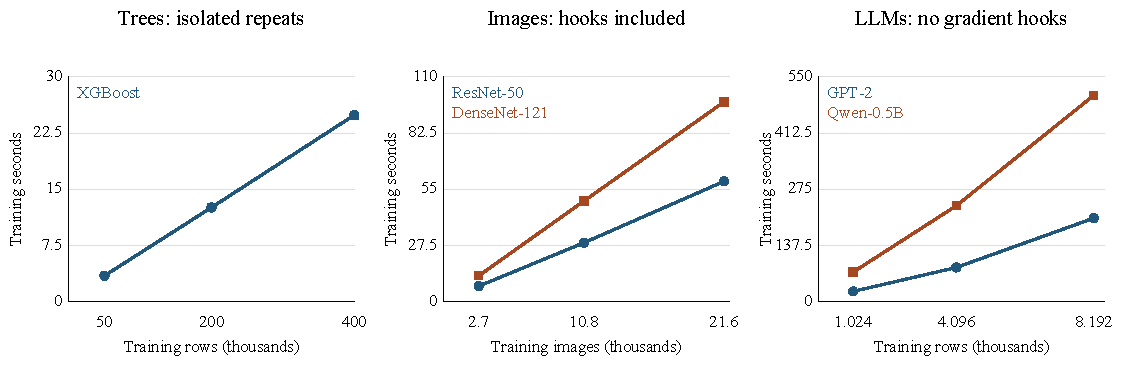
\includegraphics[width=\textwidth]{academic-scaling.pdf}
\caption{Observed local training costs, separated by workload. Tree points use
isolated medians with min--max ranges over three identical-computation timing
repetitions; image and LLM points are single runs. Image times include MRA
hooks; LLM times do not. Connecting lines describe only the measured cells,
not interpolated guarantees or a common cross-family scaling law.}
\label{fig:scaling}
\end{figure*}

\subsection{Hook Evidence and CLI Cost Have Different Boundaries}
The historical L4 language matrix replayed 3,072 forward and 3,072 backward
aggregate observations with complete registered coverage. Its three models
processed 512 optimizer steps each; measured throughput ranged from
28.96 to 42.49 rows/s. The two vision runs each recorded 507 forward and
507 backward observations; clean-test accuracy after one epoch was 0.2394
for AlexNet and 0.6898 for DenseNet-121. Full context-screen and perturbation
tables appear in the appendix. The loss-access membership profiles and
DenseNet perturbation losses motivate further evidence collection, but the
experimental screens have no clearing or blocking authority. The reported
CPU hook/non-hook control is not a CUDA noninterference proof.

\ProtocolTimingTable
All 33 historical offline chains completed 297 CLI invocations. Independent
replay checked 66 manifest signatures, 33 AuditStore chains, and 33 all-file
authenticated transcripts. Median nine-command time is 3.487 seconds at
baseline, 3.675 with 32 candidates, 3.727 with 64 threat records/192 evidence
records, and 4.067 with a 512 MiB padded artifact
(Table~\ref{tab:protocol-timing}). The totals include nine process
startups/imports; their contribution was not separately measured.
Fixture generation, historical-ledger population and
transcript construction/signing are separately measured, not included in the
nine-command total. Populating 128 prior assessments costs median 8.212
seconds; constructing/signing the longest transcript costs 0.580 seconds.
Those excluded costs rule out interpreting the totals as nearly constant
whole-lifecycle latency.

An initial memory counter measured the small Windows virtual-environment
launcher rather than the actual interpreter. Those observations are retained
as invalid for CLI-memory inference. A separately frozen single-observation
supplement measures actual-interpreter peak working set for six profiles:
51.52--59.92 MiB. It includes its measurement wrapper, excludes system caches,
and cannot be pooled with the three-repeat timing series. The benchmark predates
coverage and signing fixes; it neither repairs those defects nor measures
corrected code.

\subsection{Failures, Counterexamples, and Incomplete Evidence}
The local pre-correction focused suite recorded 136 entries: 132 passes,
one failure and three errors. A second historical suite recorded 183 entries:
179 passes and four Windows fixture-cleanup errors. These remain separate
from current regression results. The earlier import-path counterexamples
included mandatory-policy omission in a validly signed report, empty CLEAR
content, and authenticated assertions without corresponding execution.
Signature forgery was not required: a trusted benchmark key signed deficient
content. The current regression suite checks specific corrections; it is not
an exhaustive adversary campaign.

Other local public-privacy, strategic, and workflow outputs are included in the
companion inventory with their evidence status rather than promoted to
confirmatory comparisons. Configurations without completed runs, interrupted
attempts, and unavailable raw provenance do not become zero-valued rows.
The full five-model composition design and full OpenML study are not established
as completed by their configurations. Most importantly, there is no fresh
real-model run that couples all measured training scales to the corrected
four-verdict gate, authoritative registry, and live gateway. The two experiment
families cannot be concatenated after the fact to fill that gap.

\subsection{Exact Construction Details}
\label{app:construction-detail}
All seven exact checks reproduced their stated countermodel and repair control
(Table~\ref{tab:gap-constructions}). The selected-error probability is
$1-(19/20)^{20}=0.641514\ldots$ without allocation and
$1-(399/400)^{20}=0.048830\ldots$ with allocation across twenty bounds.
These are exact probabilities of the constructed procedures, not estimated
frequencies or measurements of MRA's runtime. The 42 probability bins represent
two distributions over $2^{20}$ labeled outcomes each.

The two-threat reducer uses endpoints and thresholds in $\{0,1/2,1\}$,
including reversed intervals, four missing-evidence masks, two mandatory
completion flags, four acceptance states and four actionability masks.
Its 93,312 grid cases yield 91,392 BLOCK, 1,200 RELEASE, 544
RELEASE-WITH-RISK and 176 INCONCLUSIVE decisions, with no disagreement against
the declarative cases. Ten additional boundaries test equality, invalid ranges,
absent threats, contradictions and risk-acceptance precedence. The grid is
exhaustive only for those stated finite inputs; identity, expiry, signatures
and source truth are abstracted by validity predicates. Six separate selection
controls reject an optional INCONCLUSIVE candidate, permit only properly
accepted policy-allowed optional RWR, reject unresolved mandatory RWR and
missing acceptance/policy permission, and admit an all-CLEAR RELEASE control.

The residual-atom check rejects all 255 incomplete subsets of eight supplied
scenarios and admits the full one, while the hidden-world account remains
indistinguishable. Joint decoder enumeration separates XOR disclosure from
independent noise despite identical marginal channels. Four rare-disclosure
probabilities $0.001,0.01,0.1,1$ retain posterior one; four separate binary
channels attain the additive TV expected-gain penalty. In the ideal-authenticity
construction, both accounts authenticate but complete finite-channel admission
rejects the false ceiling. A separate service-order control has one stale grant
among three split check/revoke/grant orderings, versus none among the two
atomic-grant/revocation orderings. This validates a finite race witness and
the specified serialization remedy, not a deployed gateway. These results
test the protocol's prescribed
distinctions and refusals; the general proofs, not finite success counts,
establish their all-instance scope under stated assumptions.

\section{Proof Artifacts and Evidence Provenance}
\label{app:audit}
The primary source families are: controlled finite-channel report and manifest;
v2/v3 model-backed reports, repeated replays and wrapper evidence; the curated
2 September hook audit; local public-data training/scoring reports and their
completion/verification records; the historical nine-command benchmark and
memory supplement; historical counterexample and test receipts; and the
source-bound Lean proof receipt. Historical numerical tables are generated
from \code{experimental-data.json}; the new exact finite table comes from
\code{gap-construction-results.json}. The historical inventory marks configured-only and
excluded results explicitly. A digest proves equality to inspected bytes,
not an independently authenticated measurement or a public archival deposit.

An evidence reviewer should reproduce four different checks without conflating
them: (i) regenerate tables from pinned aggregate sources; (ii) inspect all
rejected/partial attempts and non-vacuous positive controls; (iii) rebuild only
the identified Lean source with its pinned toolchain and axiom policy; and
(iv) replay the exact vintage software experiments where materials are
available. Current regression passes do not restamp historical timings.
Manuscript formatting follows the IEEE Computer Society conference class;
formatting compliance alone establishes none of these scientific checks.

\subsection{Machine-Checked Scope and Supplemental Incentives}
\label{sec:proof-status}

The results in Section~\ref{sec:theory-protocol} and the appendix are written
arguments in their stated generality, not newly kernel-checked declarations.
The existing Lean core proves unbounded inductive
reachability properties of an
abstract lifecycle and symbolic authenticated composition, and finite rational
error accounting. Its named declarations are summarized in
Table~\ref{tab:lean-scope}; no entry establishes Python refinement.

\begin{table*}[t]
\centering\small
\caption{Existing proof scope, not additional machine-checked claims from this draft.}
\label{tab:lean-scope}
\begin{tabular}{>{\raggedright\arraybackslash}p{0.18\textwidth}>{\raggedright\arraybackslash}p{0.40\textwidth}>{\raggedright\arraybackslash}p{0.34\textwidth}}
\hline
Source under \path{formal/lean/MRAP/} & Representative existing Lean declarations & Exact boundary \\
\hline
\texttt{Protocol.lean} &
\texttt{reachable\_\allowbreak authorization\_\allowbreak integrity};
\texttt{active\_\allowbreak implies\_\allowbreak committed\_\allowbreak clear\_\allowbreak and\_\allowbreak bound};
\texttt{valid\_\allowbreak active\_\allowbreak trace\_\allowbreak exists} &
All reachable abstract states satisfy registered-gate and binding invariants;
one valid active trace demonstrates nonvacuity. Gate truth is not inferred. \\
\texttt{Protocol.lean} &
\texttt{every\_\allowbreak step\_\allowbreak is\_\allowbreak role\_\allowbreak authorized};
\texttt{terminal\_\allowbreak release\_\allowbreak phase\_\allowbreak is\_\allowbreak absorbing};
\texttt{stale\_\allowbreak head\_\allowbreak second\_\allowbreak commit\_\allowbreak fails} &
Typed role/transition constraints and abstract stale-head rejection, not a
deployed identity or concurrency service. \\
\texttt{Security.lean} &
\texttt{authenticated\_\allowbreak reachable\_\allowbreak projects};
\texttt{authenticated\_\allowbreak reachable\_\allowbreak authorization\_\allowbreak integrity};
\texttt{accepted\_\allowbreak envelope\_\allowbreak replay\_\allowbreak is\_\allowbreak rejected} &
Symbolic authentication and declared compromise predicates compose with the
lifecycle. Neither Ed25519 nor compromise detection is proved. \\
\texttt{Deployment.lean} &
\texttt{successful\_\allowbreak commit\_\allowbreak is\_\allowbreak atomic\_\allowbreak and\_\allowbreak bound};
\texttt{can\_\allowbreak serve\_\allowbreak implies\_\allowbreak current\_\allowbreak live\_\allowbreak bound\_\allowbreak authorization};
\texttt{revocation\_\allowbreak stops\_\allowbreak existing\_\allowbreak gateway} &
Ideal registry/commit/gateway functions, exact identifiers and modeled time;
no concrete durable registry or serving implementation. \\
\texttt{Statistics.lean} &
\texttt{finite\_\allowbreak false\_\allowbreak authorization\_\allowbreak bound};
\texttt{registered\_\allowbreak component\_\allowbreak budget\_\allowbreak controls\_\allowbreak false\_\allowbreak authorization} &
Finite rational weighted experiments with supplied false-authorization inclusion
and justified component budgets, not inferred scientific validity. \\
\hline
\end{tabular}
\end{table*}

There is also a separate historical, output-only supplement,
\texttt{AssuranceExtension.lean}, under
\texttt{output/mrap-e2e-20260907/proof/}. Its retained successful receipt records
39 audited core declarations and 24 supplemental declarations using Lean 4.32.1.
We rechecked seven artifact hashes and all 14 recorded build-input hashes,
including source and build logs;
this is historical build evidence, not a fresh kernel run or a tracked-library
integration. The supplement proves finite-grid results corresponding to parts
of Proposition 1, predicate-profile partitions, finite ceiling lifting,
observation-only impossibility, and the four-outcome XOR witness. Representative
names are \texttt{ideal\_\allowbreak release\_\allowbreak is\_\allowbreak conditionally\_\allowbreak safe},
\texttt{profile\_\allowbreak atoms\_\allowbreak cover}, \texttt{finite\_\allowbreak coverage\_\allowbreak lifts\_\allowbreak class\_\allowbreak ceilings},
\texttt{indistinguishable\_\allowbreak unsafe\_\allowbreak world\_\allowbreak defeats\_\allowbreak universal\_\allowbreak soundness}, and
\texttt{joint\_\allowbreak export\_\allowbreak success\_\allowbreak is\_\allowbreak one}.

The qualifications matter. Its bounds are anonymous natural-number rows on an
externally normalized common probability grid; only lower--upper ordering is
checked internally. Completeness and scope coverage are supplied Booleans, and
approval/resolution is a nonempty reference, not a verified institutional
signature. The profile theorem is not connected to a proof of one identified
row per required threat. XOR marginals quantify deterministic Boolean decoders;
randomized-decoder extension is an averaging argument. The indistinguishability
lemma uses deterministic functions; the randomized version in
Appendix~\ref{app:gaps} is handwritten.
Thus this narrower target specification neither proves the current facade's
semantic replay nor establishes its equality with the historical target. No
supplement theorem proves Blackwell transfer, adaptive statistical coverage, or
Python refinement.

Specifically, \texttt{SoundOutcome.sound} supplies the implication from false
authorization to some component failure. Lean proves the weighted union-bound
consequence; it does not establish that a real experiment satisfies that premise.
The pinned toolchain is Lean 4.32.1. Parsing, canonicalization, numerical
semantics, and concrete state transitions still need a verified correspondence
before the abstract proof can cover the Python implementation. The correspondence
manifest links theorem names to concrete regression obligations; it is not a
simulation proof.

Strategic incentives remain an optional stress test. For a risk-neutral actor
whose gain from violation is at most $G^+$, end-to-end detection probability is
at least $q^-$, and effective enforceable consequence is $F\ge0$, the condition
$q^-F\ge G^++\delta$, $\delta>0$, makes violation's utility advantage at most
$-\delta$. This elementary subtraction requires credible parameter bounds and
consequences; equality without a positive margin permits indifference. It is
neither a behavioral prediction nor an authorization rule and cannot remove a
mandatory gate.

\section{Complete Aggregate Evidence Tables}
\label{app:tables}
Tables below retain supplementary measurements and adverse results, not new
replications. The companion JSON preserves additional exact values, identifiers,
source hashes, per-run timing rows and inclusion/exclusion decisions. Rounded
curated hook results are labelled as such. No raw dialogue, images, per-example
loss arrays, training rosters or private keys are included in the paper.
\SupplementaryTables
\end{document}
